\documentclass{article}
\usepackage[utf8]{inputenc}

\usepackage[spanish,es-noindentfirst]{babel}
\usepackage{graphicx}
\usepackage{longtable}
%Code Highlighting
%He tenido que quitar el Minted porque me daba error
\usepackage{lastpage}
\usepackage{placeins}
%\usepackage{biblatex}
%\addbibresource{bibliografia.bib}
\usepackage{pdflscape}
\usepackage{caption}
\usepackage{subcaption}
%Encabezados y pie de página
\usepackage{fancyhdr}               
\pagestyle{fancy}
\fancyhf{}
\fancyhead[L]{Plan de gestión, análisis, diseño y memoria del proyecto} %No cabe lo de Juego online <<Guiñote>>
\fancyfoot[L]{Grupo 11 | Susan L. Graham}
\fancyfoot[R]{\thepage \hspace{1pt} de \pageref{LastPage}}

\renewcommand{\headrulewidth}{2pt}
\renewcommand{\footrulewidth}{1pt}

\usepackage{hyperref}
\usepackage[T1]{fontenc}
\hypersetup{
    colorlinks=true,
    linkcolor=blue,
    filecolor=magenta,      
    urlcolor=cyan,
    pdftitle={Plan de gestión, análisis, diseño y memorial del proyecto <<Juego online "Guiñote">>},                   
%    bookmarks=true,
}


\title{Plan de gestión, análisis, diseño y memorial del proyecto}                            
\author{Javier Herrer Torres}      
\date{Febrero 2021}                            

\begin{document}

\begin{titlepage}
    \begin{center}
        \vspace*{1cm}
            
        \Huge
        \textbf{Juego online <<Guiñote>>}
            
        \vspace{0.5cm}
        \LARGE
		Plan de gestión, análisis, diseño y memorial del proyecto
		
        \vspace{1.5cm}
            
        \textbf{Mario Chavanel Moreno} (NIP: 679551)\\
        \textbf{Javier Fuster Trallero} (NIP: 626901)\\
        \textbf{Daniel Gracia Pardo} (NIP: 756128)\\
        \textbf{Javier Herrer Torres} (NIP: 776609)\\
        \textbf{Daniel Pérez Ramírez} (NIP: 756558)\\
        \textbf{Samuel Torres Fau} (NIP: 780505)
        
        \vfill
            
    	%Cambiar logotipo EINA por logo identificativo
    	
\includegraphics[width=0.6\textwidth]{../images/logo}
            
        \vspace{1.5cm}
            
        
         Grupo 11 | Susan L. Graham\\
        \href{https://github.com/UNIZAR-30226-2021-11}{https://github.com/UNIZAR-30226-2021-11}
            
        \vspace{1.5cm}
 
    \end{center}
\end{titlepage}

\tableofcontents

\break

\section{Introducción}
%Resumen del proyecto, propósito, alcance, objetivos, entregables e hitos principales. Alrededor de una página es suficiente. No olvidar una breve descripción de la estructura del resto del documento.
El proyecto consiste en desarrollar una aplicación multijugador y multiplataforma (Android y web) del juego del Guiñote. Además de las funciones básicas del juego relacionadas con las normas del mismo, se añadirán funcionalidades extras como pueden ser: la capacidad de pausar las partidas, consulta de perfiles de usuarios así como historiales de partidas de estos, permitir la práctica con partidas contra la IA y creación de torneos. Además de aspectos visuales de personalización para las cartas o el tablero de juego.\\

La versión inicial disponible del sistema será compatible con sistemas Android 7.0 (y posteriores) y los principales navegadores (Firefox, Chrome y Safari). El sistema generado para el proyecto constará de los siguientes componentes: API RESTful, Base de datos, clientes web y Android. Estará desplegado mediante tecnología de contenedores, dotándolo de mayor flexibilidad respecto a la plataforma de despliegue.\\

Para cumplir con este proyecto, su desarrollo se divide con 3 entregas:
\begin{itemize}
	\item 14 de marzo del 2021: Primera iteración. Análisis y diseño del sistema.
	\item 14 de abril del 2021: Segunda iteración. Desarrollo del proyecto con un primer prototipo.
	\item 1 de junio del 2021: Versión final de la aplicación. Versión final con total funcionalidad.	
\end{itemize}
Los entregables finales del proyecto serán una aplicación Android (mediante un .apk) y el servidor principal junto con la base de datos en un docker para su despliegue.\\

En este documento se describen de forma detallada los siguientes apartados:
\begin{itemize}
	\item Estructuración del equipo en grupos de trabajo para cada componente y asignación de roles principales.
	\item Planificación de la gestión del proyecto: Procesos técnicos, planes y calendario.
	\item Análisis de requisitos y diseño del sistema.
	\item Anexo: Normas del guiñote.
\end{itemize}
\section{Organización del proyecto}
%Equipo del proyecto: integrantes del mismo, roles y responsabilidades. Qué hace dentro del proyecto cada miembro del equipo. Aunque es normal que todo el mundo haga varias cosas, también es importante que haya responsables definidos para las tareas importantes. Es importante designar a un director o directora de proyecto.
El equipo encargado del proyecto está compuesto por Javier Herrer Torres, Javier Jesús Fuster Trallero, Daniel Pérez Ramírez, Samuel Torres Fau, Mario Chavanel Moreno y Daniel Gracia Pardo. \\A su vez, se han creado tres grupos de trabajo para cada una de las 3 principales partes de las que consta el proyecto:
\subsection{Backend}
Este grupo está compuesto por Javier Herrer y Javier Fuster. El objetivo principal de este grupo es el desarrollo del backend, el sistema que se encarga de gestionar las partidas de guiñote (interfaces, lógica de juego, etc). Las aplicaciones realizadas por los otros grupos se conectarán a este sistema, que ofrecerá las distintas funcionalidades indicadas en el análisis de requisitos presente en este mismo documento.

\subsection{Aplicación Web}
Este grupo está compuesto por Mario Chavanel y Daniel Gracia, y tiene el objetivo de desarrollar el cliente web que permitirá jugar al guiñote desde navegador, conectándose al backend desarrollado por el primer grupo.

\subsection{Aplicación android}
Grupo compuesto por Daniel Pérez y Samuel Torres, con la finalidad de desarrollar la aplicación android que, al igual que la aplicación web, se conectará al backend para permitir jugar desde los smartphones con sistema operativo Android.

Pese a que estén definidos los grupos y los integrantes de cada uno de estos, dado que la carga de trabajo necesaria para el desarrollo de alguna de las partes del sistema es mayor en ciertos grupos que en otros, en algunos momentos se podrá apoyar en el desarrollo de componentes de grupos ajenos.

\subsection{Director del proyecto}
El director del proyecto elegido por el grupo es Javier Herrer, mediante una votación improvisada con resultado unánime.

\subsection{Actas de reunión}
El encargado de la realización de las actas de las diferentes reuniones llevadas a cabo y de futuras reuniones es Mario Chavanel.

\subsection{Memoria}
En cuanto a la realización de la memoria no se ha establecido un responsable para la misma, cada grupo redactará y documentará las partes que le correspondan, y el resto de aspectos comunes del proyecto serán repartidos en los integrantes del mismo.

\section{Plan de gestión del proyecto}
\subsection{Procesos}
%En esta sección se describe cómo se llevarán a cabo distintas tareas que hay que realizar en distintos momentos del proyecto.
\subsubsection{Procesos de inicio}
%Cómo se van a identificar y asignar recursos (p.ej. conseguir servidores en cloud o teléfonos móviles para pruebas, pero también registrarse para acceder a API que se quieran integrar o a herramientas online que se quieran usar etc.).


%Cómo se va a abordar la formación inicial de los miembros del equipo (revisar qué tecnologías se van a usar, qué componentes se van a integrar, con qué API hay que conectar y quiénes tienen que formarse, o autoformarse, en todas esas cosas y de qué manera (hacer algún curso online, planificar algo de tiempo para auto-formación con tutoriales y documentación etc.).

En primer lugar, todos los miembros del equipo han adquirido los conocimientos básicos para la utilización de \LaTeX como lenguaje de desarrollo de la documentación necesaria para el proyecto. Para ello, se ha seguido el tutorial <<Learn LaTeX in 30 minutes>> que se puede encontrar en la página web de \textit{Overleaf}.
Además, continuando en lo que respecta a la formación común, los seis integrantes del equipo asistieron presencialmente a la práctica de la asignatura Proyecto Software, consistente en familiarizarse con la herramienta Git y su uso en conjunto con GitHub. Previamente, se habían adquirido los conocimientos necesarios para la realización
de dicha práctica asistiendo a las dos horas de clase de teoría sobre fundamentos de Git.

En lo particular, hablando de cada equipo, los encargados del desarrollo del \textit{backend} harán uso de GoLang como lenguaje de programación. Los integrantes de este equipo están familiarizados con dicho lenguaje, ya que lo utilizaron durante todas las prácticas de la asignatura Sistemas Distribuidos. Por este motivo, como formación realizaron el tutorial de la página web oficial de GoLang, \href{www.golang.org}{www.golang.org}.
Además, este equipo también se encarga del despliegue de la base de datos. Al ser de tipo SQL, ambos integrantes del equipo tienen experiencia y conocimiento suficiente debido a que cursaron la asignatura Bases de Datos durante el cuarto cuatrimestre de la titulación.

En lo que respecta al equipo de desarrollo de la aplicación Android, el aprendizaje de la herramienta Android Studio se realizó durante el quinto cuatrimestre de la titulación, mediante el curso de la asignatura Ingeniería del Software. En ella, se llevó a cabo la implementación de una aplicación de gestión de notas desde cero. Se considera que con esta base de
conocimientos y la consulta de la documentación oficial sobre el desarrollo en Android cuando sea necesario, es suficiente para poder desarrollar exitosamente el juego del guiñote en una aplicación Android.

Por último, el equipo encargado de desarrollar la aplicación web necesita adquirir los conocimientos necesarios para trabajar con HTML5, CSS y JavaScript. Aunque ambos miembros del equipo ya trabajaron con ellos durante las prácticas de la asignatura Sistemas de la Información, se considera que la experiencia adquirida no fue suficiente para desarrollar una web de la calidad suficiente, por lo que
ambos se formarán por su propia cuenta, utilizando como fuente de información los tutoriales sobre HTML, CSS y JavaScript que aparecen en la página web \href{www.developer.mozilla.org}{www.developer.mozilla.org}, dentro de la sección <<Tecnologías Web>>.


\subsubsection{Procesos de ejecución y control}
%Cómo se llevarán a cabo las comunicaciones internas, el registro de las decisiones tomadas en reuniones, la redacción de las actas etc.

%Cómo se van a determinar las tareas a realizar y el reparto de las mismas a integrantes del equipo en el día a día.

%Cómo se abordarán los temas de gestión del equipo humano (p.ej. la resolución de disputas).

%Qué se va a hacer respecto a medidas de progreso y monitorización del estado del proyecto (qué se mira/mide, cada cuánto tiempo, qué se hace si se detectan problemas de rendimiento o avance insuficiente o desviaciones respecto al plan inicial...).

%Cómo se hará la entrega de resultados.


Las comunicaciones internas se realizarán mediante la aplicación de mensajería instantánea WhatsApp, a través del grupo creado a tal efecto. Además, se realizarán reuniones en el \textit{slot} acordado la primera semana, en el que todos los miembros están disponibles: martes de 12:00 a 14:00 (en la hora de seminario). El contenido de estas reuniones será recogido por Mario Chavanel Moreno, que se encargará de la redacción de actas cuyo contenido incluirá las decisiones tomadas.

Además, el equipo usará GitHub como herramienta de apoyo para la asignación de las tareas a realizar. El director del proyecto, Javier Herrer Torres, creará las \textit{issues} correspondientes. Además, podrá asignarla a un equipo en concreto (\textit{frontend} o \textit{backend}) o podrán ser los propios integrantes los que se auto asignen las tareas que más les interesen.

Las posibles disputas que surjan sobre, por ejemplo, aspectos funcionales relevantes del proyecto, serán discutidas con todos los miembros del equipo dando razones a favor y en contra de tomar una determinada acción. Y, posteriormente, se someterá a votación escogiendo la opción con más votos.

También se empleará GitHub para el seguimiento del progreso y el estado del proyecto mediante \textit{Milestones} que permiten ver de forma gráfica este progreso. Además, GitHub proporciona gráficas y métricas en base a los \textit{commits} de los colaboradores.

Cuando un colaborador complete una tarea asignada, unirá sus cambios con la rama \textit{master} del repositorio marcando la \textit{issue} como cerrada. Las tareas podrán ser revisadas por el director del proyecto o por cualquier otro integrante relacionado con esa tarea.

\subsubsection{Procesos técnicos}

\paragraph*{Redacción de memorias y documentación}
Para el desarrollo de la memoria del proyecto y de todo el resto de documentos empleados se empleará el lenguaje de \LaTeX, ya que se trata de una lenguaje orientado a la creación de documentos escritos, y proporciona una alta calidad tipográfica.
Debido a la elección de este lenguaje, se trabaja sobre ficheros \texttt{.tex} directamente, empleando GitHub para el trabajo colaborativo, al igual que con el resto del código del proyecto. El compilador empleado para generar los ficheros PDF es MikTex.

\paragraph*{Empleo de GitHub}
Para el control de versiones y configuraciones va a hacerse uso de GitHub. Del mismo modo también será empleado para el trabajo colaborativo.


\paragraph*{Desarrollo del backend}
El backend va a crearse en el lenguaje de programación \href{https://golang.org/dl/}{GoLang (1.16.3)}, por lo que el grupo responsable del mismo ha optado por emplear el \href{https://www.jetbrains.com/es-es/go/}{IDE GoLand} de JetBrains, en su versión 2020.3.4, ya que está específicamente enfocado en este lenguaje. La elección de GoLang se debe a la facilidad que ofrece para el despliegue de componentes web.

En lo respectivo a la base de datos del backend, va a emplearse \href{https://www.postgresql.org/download/}{PostreSQL}, en su versión 13.X, ya que, además de ser software libre, ofrece las funcionalidades necesarias para el proyecto.



\paragraph*{Desarrollo de la aplicación Android}
Para el desarrollo del cliente Android va a emplearse el lenguaje \href{https://www.java.com/es/}{Java}, ya que está ampliamente soportado en los dispositivos con sistema operativo Android y que ofrece un buen soporte para el desarrollo de aplicaciones nativas. Además, se empleará la base de datos de los teléfonos inteligentes para guardar la información de la aplicación, es decir, se hará uso de SQLite si es necesario.

Respecto al desarrollo de la aplicación, va a trabajarse con \href{https://developer.android.com/studio}{Android Studio} en su última versión (4.1.3), ya que se trata de un IDE muy completo y que proporciona funcionalidades de gran utilidad, como la integración de emuladores Android, que facilitan la creación de aplicaciones. El emulador empleado para el testeo de la App simula el SmartPhone Google Pixel y emplea la API 24 (Android 7.0).

\paragraph*{Desarrollo de la aplicación Web}
La aplicación web va a ser desarrollada en HTML5 y CSS3, dado que son el estándar para el desarrollo web. Además se hará uso de JavaScript para ayudar a crear las funcionalidades del juego, así como \href{https://262.ecma-international.org/7.0/}{ECMAScript 2016}.

En cuanto al desarrollo del código, va a hacerse uso de \href{https://code.visualstudio.com/Download}{Visual Studio Code} en su última versión (1.55.0), con los plugins pertinentes que faciliten el desarrollo web, como la visualización de las páginas HTML. Se ha decidido emplear este editor por el gran número de plugins de los que dispone, así como por la facilidad de uso de la herramienta en cuestión.

\subsection{Planes}
%Un plan establece un objetivo y, en general, qué necesitamos para conseguirlo. Llevar a cabo los planes que se describan aquí requerirá aplicar los procesos descritos anteriormente, algunos una vez y otros muchas veces. Un plan suele incluir cuándo se llevan a cabo estos procesos (periódicamente, o en fechas concretas, o “al menos N veces” etc.) y quién es responsable (personas concretas a veces, pero generalmente roles) de hacerlos, o de asegurarse que se hacen.

\subsubsection{Plan de gestión de configuraciones}
%Convenciones de nombres (documentos) y estándares de código (guías de estilos).


%Responsable o responsables de las distintas actividades (puesta en marcha, apoyo al equipo, revisión de commits, copias de seguridad, control de las versiones entregadas a cliente...).

%Recursos: repositorios de control de versiones (cuáles, cuántos, permisos de acceso a los mismos) y sistema de gestión de incidencias.

%Procedimiento para realizar cambios al código fuente y los documentos técnicos: workflow de control de versiones utilizado, cuándo/cómo se permiten realizar commits al repositorio compartido, si tienen que ser aceptados por alguien previamente o no, qué hay que anotar en el sistema de gestión de incidencias, quién decide el estado de las incidencias, en qué estados puede estar una incidencia etc.

Toda la gestión del proyecto y el control de las versiones y configuraciones se va a realizar utilizando \textit{GitHub}. El proyecto constará de 4 repositorios que estarán guardados dentro de una organización llamada UNIZAR-30226-2021-11.

Un repositorio será exclusivamente para la documentación, que será realizada utilizando \LaTeX. Todos los miembros del equipo modificarán el repositorio siguiendo un flujo de trabajo centralizado.

Los otros tres repositorios estarán dedicados al código del proyecto, un repositorio será dedicado al \textit{backend} y los otros dos al \textit{frontend}(app movil y app web). Los integrantes del equipo se han dividido en sub-grupos de dos personas y cada sub-grupo trabajará sobre su propio repositorio y será el encargado de garantizar un correcto control de las versiones. Para estos repositorios se utilizará un flujo de trabajo con ramas, de modo que para cada nueva funcionalidad que se vaya a añadir se creará una rama nueva y una vez esté completa se juntará con la rama principal.

Para el reparto de las tareas se utilizarán las \textit{issues} de \textit{GitHub}. Cada \textit{issue} representará una funcionalidad o una tarea a desarrollar. Cuando un miembro del grupo vaya a realizar una de ellas deberá asignársela y cuando la haya completado deberá cerrarla. Además, esta herramienta permite realizar comentarios para facilitar la comunicación entre los miembros del equipo.

\subsubsection{Plan de construcción y despliegue del software}
%Cómo se construye e integra el software: si hay scripts de construcción automatizada o no (en ese caso qué se usa, y cómo se garantiza que todos los participantes compilan igual y con las mismas dependencias), qué se incluye en la construcción (descarga y actualización de dependencias, compilación, ejecución de tests automáticos...) y cada cuánto se construye (compila, integra, prueba) el sistema completo, cómo se configuran los computadores de los desarrolladores.

%Cómo se despliega el software más allá de las máquinas de desarrollo: contenedores, máquinas virtuales, servidor en cloud etc. y cómo se configuran esos entornos (rutas, usuarios y contraseñas, puertos y otros elementos).

El \textit{backend} de la aplicación se encontrará desplegado dentro de un contenedor de Docker, que recibirá las peticiones mediante \emph{nginx}. Estará situado en un servidor, ya sea de uno de los integrantes o de un proveedor de este tipo de servicios como AWS. El objetivo es que, los desarrolladores de \textit{frontend} puedan probar el correcto funcionamiento de la aplicación realizando peticiones a un mismo servidor.

Este servidor se actualizará siguiendo una \emph{integración continua}. Es decir, cada \textit{commit} en la rama \textit{main} del repositorio de \textit{backend} provocará la ejecución de un script de construcción automatizada para modificar el despliegue. Esto garantiza que todos los participantes puedan observar el resultado al mismo tiempo que programa.

Los computadores de los desarrolladores estarán configurados con el mismo IDE: Android Studio para la aplicación móvil, Visual Studio para la aplicación web, y GoLand para el \textit{backend}. Además, deberán hacer uso de GitHub para subir los cambios que realicen.

La aplicación móvil se encontrará disponible en la tienda de aplicaciones de Android, Google Play. La aplicación web será accesible mediante una URL desde un navegador como Google Chrome. Todo el almacenamiento de información relativa a usuarios, contraseñas, etc. se encontrará en el servidor común al que podrán realizar peticiones en las rutas especificadas.


\subsubsection{Plan de aseguramiento de la calidad}
%Guías para la documentación de diseño del software y otros documentos del proyecto, guías para el diseño gráfico de las GUI (estética, usabilidad...).

%Actividades de control de calidad del código que se realizarán: revisiones de código por pares, revisiones de requisitos o diagramas UML por pares, tipos de tests automáticos o manuales que se llevarán a cabo.

Pruebas de integración de la API con las aplicaciones web y Android. Estas pruebas consistirán en asegurar que se establece la comunicación entre el servidor y los clientes y que las peticiones y respuestas son correctas. Esta prueba se debe realizar una vez finalizada la comunicación entre clientes y servidor y está prevista para la primera iteración. Para ello se han utilizado las siguientes herramientas:
\begin{itemize}
	\item \textit{Postman:} es una herramienta que permite realizar peticiones al API y visualizar los datos recibidos sin necesidad de crear un cliente.
	\item \textit{Android Profiler:} es una utilidad de android studio que permite monitorizar el tráfico de red. 
	\item \textit{Wireshark:} es un analizador de paquetes para visualizar los datos que se envían y reciben entre la API y el \textit{front-end web}. 
\end{itemize}  

Inspección de código para evitar posibles errores que no ha detectado el compilador o se pueden producir en tiempo de ejecución. Estas revisiones se realizarán por parejas, cuando se añada una funcionalidad nueva al sistema.

Pruebas de usabilidad de las interfaces, para verificar que se puede acceder a todos los requisitos especificados y no existe ningún bug, alguna secuencia de acciones que pueda ocasionar algún error en la interfaz o que exista alguna pantalla inaccesible.La prueba se realizará una vez finalizada la interfaz.

Pruebas de funcionamiento para cada nuevo requisito que se realice en el sistema. Estas pruebas se realizarán a lo largo de toda la fase de desarrollo cada vez que se termine de implementar un requisito o una nueva funcionalidad. En concreto:
\begin{itemize}
	\item \textbf{Particiones de equivalencia:} en las funciones que se encarguen de comunicarse con el servidor (API), para verificar que los datos enviados y recibidos son los correctos y comprobar que sucede en caso de un mensaje invalido.
	\item \textbf{Pruebas unitarias:} en cada función del \textit{back-end} en la parte encargada de la simulación, utilizando la librería estándar de Goland (go test). Estas consisten en pruebas de caminos, para garantizar que por lo menos se ejecuta una vez cada sentencia del sistema y pruebas de simulación en la que se realiza una partida real pasando por todos los estados del autómata diseñado. Estas pruebas son de gran importancia porque la simulación del juego es la parte más importante del proyecto y hay que asegurar su correcto funcionamiento.  
	\item \textbf{Prueba de valores límite, valores típicos de error y valores imposibles:} en aquellas partes del \textit{front-end} donde tiene que interactuar el usuario insertando datos de forma manual, como por ejemplo al registrarse, iniciar sesión, buscar el perfil de algún usuario...
\end{itemize}

\subsubsection{Calendario del proyecto y división del trabajo}
%Diagrama de Gantt que recoja las tareas a realizar. Tened en cuenta que trabajáis con dos iteraciones y por tanto que hay una entrega intermedia y una final, y esto debe estar reflejado en este diagrama. Tened en cuenta que es normal que lo tengáis que actualizar conforme avance el proyecto (cuándo y cómo establezcáis en la sección 3.1.2 (Procesos de ejecución y control).
	%Debe quedar claro qué requisitos van a estar completados en la primera iteración y cuáles en la segunda. Es posible que para la primera iteración no se planifique completar ningún requisito, pero en ese caso tiene que planificarse qué se hará y que faltará por hacer para cada requisito.

%División del trabajo en partes (los módulos del software a desarrollar, pero también la documentación, el diseño gráfico, instalaciones o despliegues, pruebas manuales etc.) y reparto de los mismos entre el equipo de desarrollo, al menos a alto nivel (el reparto de labores concretas en el día a día no se detalla aquí, pero hay que explicar bajo qué criterios y quién/cómo se hace eso en la sección 3.1.2 (Procesos de ejecución y control). Debe haber una correspondencia con las tareas que aparecen en el diagrama de Gantt (que no necesariamente tiene que ser una relación uno a uno).
	%Verificad que esta división del trabajo cubre todos los requisitos.
Se va a realizar una planificación de los trabajos a realizar por cada equipo, que
podrá ser modificado en caso de fallos en la planificación, retrasos o
adelantos. En todo caso, quedaría reflejado en el diagrama de Gantt.

La división de trabajos se va a realizar por equipo, \textit{frontend web},
\textit{frontend} android y \textit{backend}. Cada equipo tendrá su propio calendario interno, coincidiendo en 2 fechas clave:
14 de abril, para una primera prueba de integración entre \textit{frontend} y \textit{backend}.

Habrá unos hitos iniciales:
\begin{itemize}
    \item Creación repositorios. Fecha est. 21/03
    \item Creación de \textit{scripts} de despliegue automático. Fecha est. 31/03
    \item Primera prueba integración. Fecha est. 10/04
\end{itemize}

\paragraph{Calendario equipo android}

Las tareas de éste equipo son las siguientes:
\begin{itemize}

    \item Implementación de wireframe. Fecha est. 25/04
    \item Diseño inical interfaz. Fecha est. 1/04
    \item Implementación capa acceso API. Fecha est. 10/04
    \item Primera integración. Fecha est. 13/04
    \item Desarrollo perfil de usuario. Fecha est. 1/05
\end{itemize}

\paragraph{Calendario equipo web}

Las tareas de éste equipo son las siguientes:
\begin{itemize}

    \item Implementación de wireframe. Fecha est. 25/04
    \item Diseño inical interfaz. Fecha est. 1/04
    \item Implementación capa acceso API. Fecha est. 10/04
    \item Primera integración. Fecha est. 13/04
    \item Desarrollo perfil de usuario. Fecha est. 1/05
\end{itemize}
\paragraph{Calendario equipo backend}


Las tareas de éste equipo son las siguientes:
\begin{itemize}
    \item Definir e implementar el modelo de datos. Fecha est. 22/03
    \item Desplegar y configurar el servidor Ubuntu. Fecha est. 25/03
    \item Puesta en funcionamiento del servidor web. Fecha est. 25/03
    \item Implementación la API-Restful. Fecha est. 10/04
    \item Implementación de la lógica de juego. Fecha est. 30/04
    \item Implementación de la inteligencia artificial. Fecha est. 15/05
    \item Implementación de los torneos. Fecha est. 30/05
\end{itemize}


\paragraph{Diagrama de Gantt}
El seguimiento de estas tareas se va a realizar mediante un diagrama de Gantt,
en el cual se reflejaran los posibles adelantos o retrasos en las tareas, así
como las tareas imprevistas que pudiesen surgir durante la realización del
proyecto.

El diagrama de Gantt final se encuentra en el anexo \ref{anexo:Gantt}.


\section{Análisis y diseño del sistema}
\subsection{Análisis de requisitos}
%Hay que completar y detallar los requisitos preliminares incluidos en la propuesta técnica y económica. Recordad que los requisitos deben ser completos, concretos, medibles cuando tenga sentido y lo menos ambiguos posible. También es importante que estén identificados para facilitar su trazabilidad.

\subsubsection{Requisitos funcionales} % Requisitos funcionales
\begin{center}
    \begin{longtable}{ | p{0.15\textwidth} | p{0.85\textwidth} | }
        \hline
        \textbf{Código} & \textbf{Descripción} \\
        \hline
        RF-1 & El sistema implementará la funcionalidad completa del juego del Guiñote, respetando todas las normas del juego original. \\
        \hline
        RF-2 & Las partidas consistirán en competiciones entre cuatro personas, organizadas en 2 parejas. \\
        \hline
        RF-3 & El sistema determinará y notificará cuál ha sido la pareja ganadora al finalizar cada partida. \\
        \hline
        RF-4 & El sistema permitirá jugar contra la CPU, pudiendo existir una, dos o tres inteligencias artificiales que desempeñen la función de un jugador. \\
        \hline
        RF-5 & El sistema permitirá pausar la partida para retomarla posteriormente. Para ello, será necesaria la confirmación de, al menos, un miembro de la pareja contraria a la que realizó la petición de pausa.
        Para su reanudación, todos los participantes deberán ponerse de acuerdo. El sistema garantizará que todas las características de la partida se conserven tal y como se encontraban justo antes de la pausa. \\
        \hline
        RF-6 & El sistema permitirá que cada jugador pueda personalizar su interfaz gráfica en el juego. Se podrán cambiar los siguientes aspectos: color y diseño del reverso de las cartas y color y diseño del tapete. \\
        \hline
        RF-7 & El sistema guardará un histórico de los resultados de las partidas de cada jugador. En cada entrada de dicho registro, figurarán los siguientes parámetros: duración de la partida, pareja ganadora y puntuación final. \\
        \hline
        RF-8 & El sistema permitirá consultar el histórico completo de un jugador, pero solamente desde el perfil de dicho jugador. \\
        \hline
        RF-9 & El sistema permitirá la participación en torneos. Para ello, un usuario deberá realizar la inscripción indicando el nombre de usuario de su pareja de juego, lo que enviará una invitación a dicho usuario. Una vez acepte, podrán comenzar a jugar.
        El sistema de juego será el siguiente: ocho parejas participarán en un mismo torneo con formato eliminatorio, es decir, para ganar un torneo habrá que ganar cuartos de final, semifinal y final. \\
        \hline
        RF-10 & El sistema requerirá un \textit{login} al comienzo de cada sesión de juego, lo que permitirá acceder a los usuarios utilizando su nombre de usuario y contraseña. En consecuencia, la creación de una cuenta será absolutamente obligatoria para poder jugar. \\
        \hline
        RF-11 & El sistema dará la opción al usuario de recordar sus credenciales para no tener que iniciar sesión cada vez que lance la aplicación, ya sea a través de la web o de la aplicación móvil. \\
        \hline
        RF-12 & El sistema, una vez un usuario haya terminado de crear una cuenta, enviará un correo electrónico de confirmación a la dirección utilizada para crear el perfil. Mientras no se realice la confirmación, dicho usuario no podrá jugar ningún tipo de partida ni participar en torneos. \\
        \hline
        RF-13 & El sistema almacenará las contraseñas de las cuentas de los usuarios de forma segura en la base de datos utilizando cifrado de una sola dirección, es decir, almacenando contraseñas con \textit{Hash}. \\
        \hline
        RF-14 & El sistema permitirá que un jugador pueda buscar el perfil de cualquier otro jugador mediante su nombre de usuario. \\
        \hline
        RF-15 & El perfil de un jugador mostrará su nombre de usuario y un histórico de las diez últimas partidas jugadas en el que figurará, para cada partida, la duración, los nombres de usuario de las parejas enfrentadas, la pareja ganadora y la puntuación final. \\
        \hline
        RF-16 & El sistema mostrará las reglas del juego del guiñote si un usuario así lo solicita. \\
        \hline
        RF-17 & El sistema ofrecerá al usuario la opción de cerrar la sesión actual, siempre que este no se encuentre en partida. \\
        \hline
        RF-18 & En el caso de producirse una desconexión, el jugador en cuestión será sustituido por la inteligencia artificial. \\
        \hline
        RF-19 & El sistema permitirá buscar partidas concretas mediante el código la misma para unirse a ella. \\
        \hline
        RF-20 & El sistema permitirá a los usuarios realizar el borrado de la cuenta con la que se registraron, lo que implicará el borrado de todos los datos almacenados en la base de datos que estén relacionados con su perfil (correo electrónico, contraseña y otros datos personales, 
        pero no partidas en las que el usuario haya participado, ya que representan datos que también se encuentran relacionados con el resto de usuarios del sistema). \\
        \hline
        \caption{Tabla de Requisitos Funcionales}
    \end{longtable}
\end{center}

\subsubsection{Requisitos no funcionales} % Requisitos no funcionales
\begin{center}
    \begin{longtable}{ | p{0.15\textwidth} | p{0.85\textwidth} | }
        \hline
        \textbf{Código} & \textbf{Descripción} \\
        \hline
        RNF-1 & El sistema permitirá jugar partidas contra otros usuarios, contra usuarios e inteligencia artificial o solamente contra Inteligencia Artificial. \\
        \hline
        RNF-2 & El juego será accesible desde aplicación móvil y desde aplicación web. \\
        \hline
        RNF-3 & La aplicación web funcionará en navegadores Google Chrome, Mozilla Firefox y Safari. \\
        \hline
        RNF-4 & La aplicación móvil funcionará únicamente en sistemas operativos Android con versión mínima 7.0. \\ % versiones mínimas????
        \hline
        RNF-5 & Cuando una partida sea pausada, se podrá retomar desde la aplicación móvil si fue pausada en la aplicación web y viceversa. \\
        \hline
        RNF-6 & Las partidas se realizarán de manera síncrona, es decir, los jugadores deberán coincidir en el tiempo mientras se desarrolla la partida. \\
        \hline
        RNF-7 & Todos los datos relativos al sistema (nombres de usuario, contraseñas, datos de los perfiles, estadísticas de partidas, etc.) estarán almacenados en una base de datos tipo SQL. \\
        \hline
        RNF-8 & Los usuarios registrados tendrán acceso a un conjunto de operaciones restringido. Podrán jugar partidas, participar en torneos, consultar y modificar su perfil y consultar perfiles de otros usuarios. \\
        \hline
        RNF-9 & La aplicación web cumplirá las <<Recomendaciones del W3C>> en lo relativo a versiones de HTML, CSS, etc. \\
        \hline
        RNF-10 & La aplicación web seguirá el estándar de accesibilidad WCAG 2.0, establecido por el W3C. \\
        \hline
        RNF-11 & Tanto la web como la aplicación móvil tendrán su interfaz gráfica bien estructurada, organizando el contenido por pestañas que abarquen todas las funciones disponibles. \\
        \hline
        
        \caption{Tabla de Requisitos No Funcionales}
    \end{longtable}
\end{center}

\subsection{Diseño del sistema}
%Diagramas arquitecturales (de módulos, de componentes y conectores, de distribución), patrones de diseño y estilos arquitecturales que se aplicarán. Las interfaces (de módulos y de componentes) son especialmente importantes. También lo son los protocolos de comunicación entre componentes.


El sistema está pensado para facilitar el despliegue en diferentes máquinas
fácilmente usando Docker.

\subsubsection{Diagramas arquitecturales}
%Tecnologías elegidas (lenguajes de programación, componentes que se integrarán, API web externas con las que se conectará etc.).

% Tabla de componentes
El sistema tiene 6 componentes principales relacionados de la siguiente manera:
\begin{figure}[htb]
    \centering
    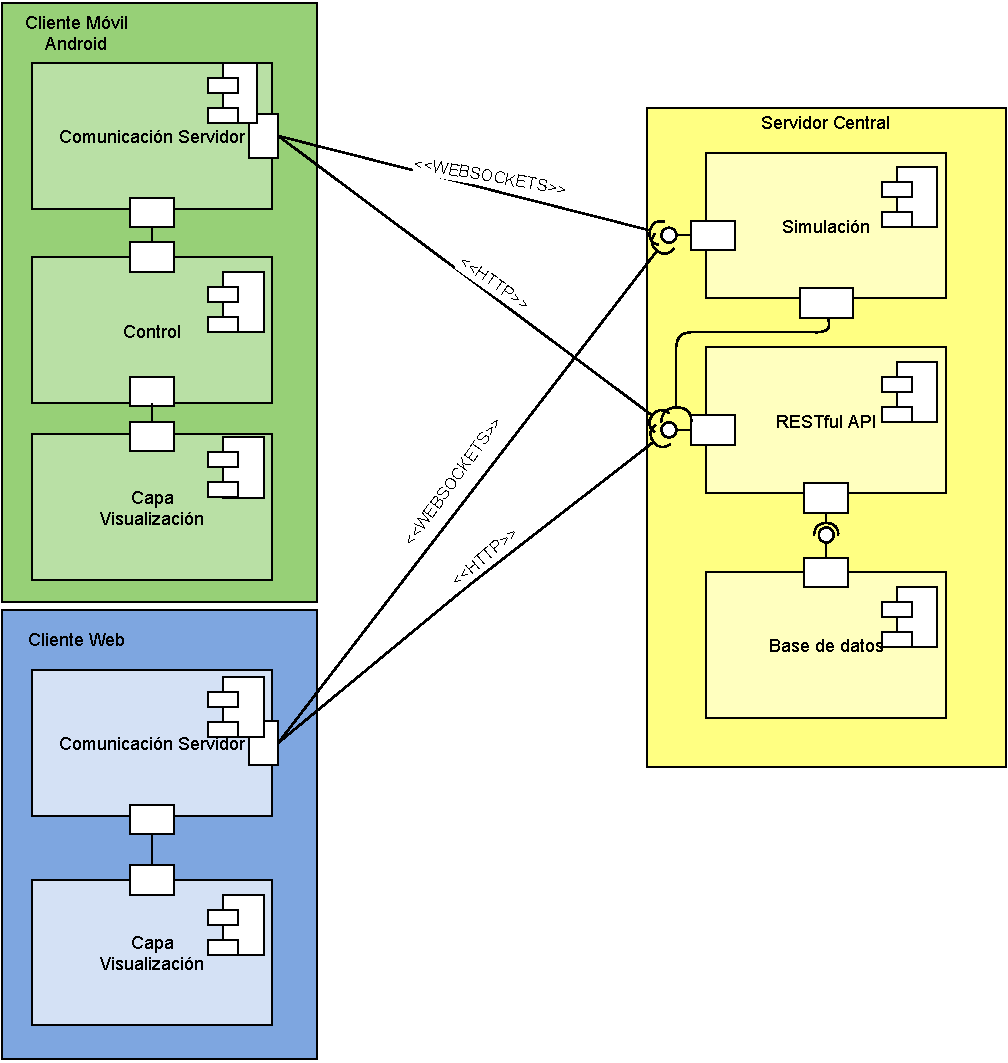
\includegraphics[width=0.8\textwidth]{../images/componentes_despliegue.pdf}
    \caption{Diagrama de componentes}
    \label{fig:diag_componentes}
\end{figure}

Un servicio REST que ofrece una interfaz de acceso CRUD a todos los datos necesarios para
el funcionamiento de los clientes, su funcionalidad detallada aparece en la sección \ref{REST_API}
Cada cliente implementará su propia capa de acceso a la API, con la que se comunican mediante
HTTPS.

\begin{figure}[htb]
    \centering
    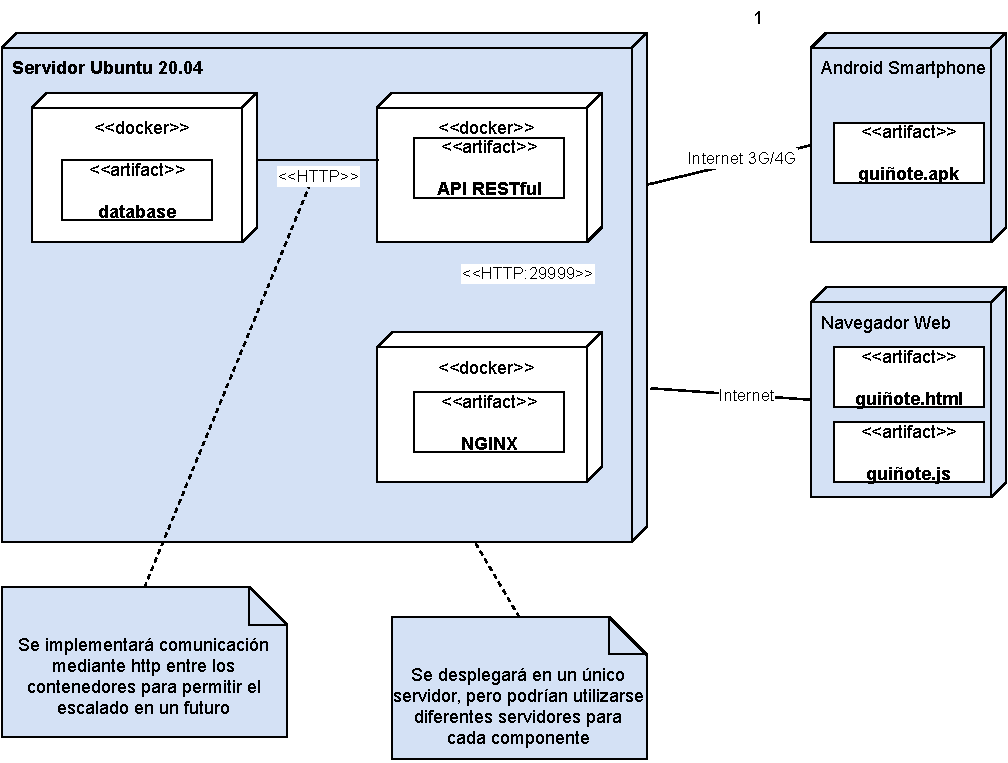
\includegraphics[width=0.8\textwidth]{../images/diagrama_despliegue.pdf}
    \caption{Diagrama de despliegue}
    \label{fig:diag_despliegue}
\end{figure}

Los clientes se conectarán mediante https al contenedor NGINX, con funcionalidad
únicamente de proxy inverso, redireccionando las peticiones a los diferentes endpoints.
El servidor web será una sencilla aplicación que servirá las páginas presentes
en diferentes directorios, será implementado en Go.

Nunca se permitirán conexiones desde el exterior a la base de datos para impedir ataques sobre ella. 

\FloatBarrier
\subsubsection{Tecnologías elegidas}

El proyecto se va a desarrollar con diferentes lenguajes de programación, esto se hace para aprovechar las 
fortalezas de cada uno en su campo de aplicación así como la experiencia disponible en el equipo de desarrollo.


\paragraph*{Aplicación Web}

Está dividida en vista y controlador, el modelo del juego estará implementada en el \textit{backend}, 
la lógica de la interfaz web será implementada con JavaScript nativo en todos los navegadores. 
La interfaz será implementada con las tecnologías tradicionales web, HTML y CSS.

\paragraph*{Aplicación Android}
El desarrollo de aplicaciones Android nativo, se puede realizar mediante dos tecnologías:

\begin{itemize}
    \item Java
    \item Kotlin
\end{itemize}

Debido a que en el equipo de desarrollo se tiene mucha más experiencia con Java que con Kotlin, y realizar 
el desarrollo con un lenguaje diferente a estos dos representa una serie de complicaciones no deseadas, 
posibles incompatibilidades de llamadas, necesidad de librerías extensas y manejo de dependencias adicionales, se realizará .

\paragraph*{RESTful API} \label{REST_API}

Para este componente se han barajado distintas opciones, ya que no está tan marcado por la plataforma sobre la que se despliega como los componentes de la interfaz.
\begin{itemize}
    \item Java, es uno de los lenguajes más utilizados en backend, existe familiaridad en el equipo con el aunque es un lenguaje con mucha verbosidad, requiere
        de una máquina virtual para su ejecución. Así mismo las implementaciones nativas de servidores web requieren del despliegue de un servidor en Tomcat con
        las implicaciones que pueda tener.
    \item Golang, un lenguaje relativamente novedoso, ampliamente utilizado por empresas trabajando en desarrollo de tecnologías en la nube, es un lenguaje 
        compilado, por lo que no requiere de una máquina virtual, y a su vez posee unas librerías estándar pensadas para el desarrollo de aplicaciones que 
        necesitan conectividad, además el equipo de desarrollo también tiene experiencia en él.
\end{itemize}

Debido a que es necesario el diseño y desarrollo de una API RESTful en poco tiempo y se posee el mismo conocimiento en ambos, se ha decidido utilizar Golang ya que su librería estándar presenta grandes facilidades a la hora de crear servicios web y su despliegue consiste en ejecutar el binario creado.

\paragraph*{Servidor Web}

Como servidor web tras la elección de Golang como lenguaje para la API se nos presentan dos opciones:

\begin{itemize}
    \item Un servidor web tradicional como NGINX o Apache.
    \item Creación de nuestro propio servidor.
\end{itemize}

Debido a las restricciones de los plazos, se utilizará NGINX para agilizar el despliegue, debido a que permite el despliegue de diferentes servicios en la misma
máquina física.

Actuará como proxy inverso para todos los servicios disponibles en la máquina. Preferiblemente, la conexión se realizará siempre mediante el protocolo HTTPS, para asegurar la
privacidad de las conexiones.

\paragraph*{Base de datos}

En primer lugar se ha decidido entre usar una base SQL o NoSQL, debido a que nuestro modelo de datos no requiere de la realización de grandes consultas 
SQL, ni la necesidad del escalado que ofrecen las NoSQL, se ha optado por la opción más familiar, una base de datos relacional tradicional.

La implementación a elegir:

\begin{itemize}
    \item PostrgeSQL
    \item MySQL
\end{itemize}

Se ha optado por PostgreSQL porqué el equipo tiene mayor experiencia en ella y es ampliamente usada en servicios en producción.


\subsubsection{Mapa de navegación}
El mapa de navegación  con las pantallas de la aplicación se encuentra en el
anexo \ref{anexo:navegacion}.

%Otros aspectos técnicos de interés (p.ej. si hay base de datos si va a ser SQL o NoSQL, si hay una API Web va a ser REST[ful] o no, si algunas de las operaciones van a ser asíncronas o no, si va a ser una aplicación móvil o de escritorio será nativa o se van a usar tecnologías web, cómo se van a considerar los requisitos de seguridad o de prestaciones, cómo y dónde se harán las instalaciones y despliegues etc.)

%Hay que justificar todas las decisiones de diseño. Esto exige contestar a dos preguntas sobre cada decisión: ¿qué alternativas se barajaron? y ¿por qué se eligió una y no las otras?


\section{Memoria del proyecto}
%En este capítulo se describirá cómo se ha llevado a cabo el proyecto, qué cambios se han hecho respecto a la versión inicial, imprevistos surgidos, etc.

\subsection{Inicio del proyecto}
%Describir cómo transcurrió esta fase del proyecto, especialmente los resultados de llevar a cabo los procesos descritos en la sección 3.1.1 (Procesos de inicio).
Los integrantes del proyecto no tuvieron problemas en la utilización de la herramienta GitHub ya que habían adquirido los conocimientos necesarios en la práctica de la asignatura. Sin embargo, sí que tuvieron ciertas dificultades en el aprendizaje de \LaTeX para la redacción de este documento. Estas dudas fueron resueltas por el coordinador del proyecto.

El equipo de Backend no necesitó aprender de cero el lenguaje de programación GoLang ya que lo habían empleado en la asignatura de Sistemas Distribuidos. Además, mostraron gran interés en el aprendizaje de nuevos usos y aplicaciones de este lenguaje como es, por ejemplo, la creación de una APIRest o la implementación de la lógica del juego. Por otro lado, para el diseño de las consultas SQL fueron suficientes los conocimientos adquiridos en la asignatura de Bases de datos.

De la misma manera, el equipo de Android tampoco partió de cero en el desarrollo de la aplicación ya que pudo emplear lo aprendido en la asignatura de Ingeniería del software, concretamente en el trabajo de la asignatura. También tuvieron que investigar acerca de nuevas tecnologías y librerías para la implementación de las peticiones al Backend.

Por último, el equipo encargado de desarrollar la aplicación Web pudo emplear también el trabajo de la asignatura de Sistemas de Información.

Se realizó una reunión antes de Semana Santa en la que se fijaron las bases para empezar a trabajar en el desarrollo del proyecto. El equipo de Backend redactó una documentación en la que incluyó información acerca de las peticiones (método, formato, cuerpo del mensaje, respuesta...) para que los dos equipos de Frontend pudieran ir probando su código. También se propuso la idea de realizar integración continua de forma que el Backend estuviese disponible en línea a través de una dirección pública, pero se ha dado prioridad a la implementación del mismo. 




\subsection{Ejecución y control del proyecto}
%Describir cómo transcurrió esta fase del proyecto, especialmente los resultados de llevar a cabo los procesos descritos en la sección 3.1.2 (Procesos de ejecución y control) y en la sección 3.1.3 (Procesos técnicos). No olvidar:
%Cómo se ha realizado el reparto de trabajo entre miembros del equipo. Cómo ha transcurrido la comunicación interna.
%Cómo se ha medido el progreso del proyecto. Cómo se sabía el trabajo realizado, el trabajo pendiente y lo que estaba haciendo cada persona.
%Los ajustes realizados cuando se detectaron divergencias frente al calendario inicial (ajustes en el trabajo y/o ajustes en el calendario). Si se han identificado las causas de estas divergencias, explicarlas.
%Adecuación de las herramientas y tecnologías empleadas. Si ha habido que cambiar alguna decisión de diseño o tecnología, y por qué.
%Funcionamiento de los procesos de control de versiones del código, construcción y despliegue. ¿Ha habido problemas con las integraciones? ¿Problemas con los despliegues? ¿Se han perdido cosas por errores humanos? ¿Cómo se han abordado estas tareas?
%Pruebas del software. ¿Se han podido cumplir las ideas que se tenían al respecto?

El equipo ha trabajado dividido en tres grupos, cada uno encargado de desarrollar una tarea distinta (aplicación android, aplicación web y \textit{backend}). Esta organización de trabajo ha sido correcta y aplicable para próximos proyectos, sin embargo habría que considerar aumentar la frecuencia de las reuniones de seguimiento. Durante las primeras semanas de trabajo el numero de reuniones fue insuficiente y como consecuencia se produjeron algunos errores de comunicación entre los grupos. Esta situación se soluciono las ultimas semanas reuniendo a todos los equipos con mayor frecuencia.

Para la comunicación se han utilizado dos aplicaciones. Para mensajes sencillos y consultas breves se ha creado un grupo de Whatsapp para el proyecto. Para reuniones o para comunicarse con los compañeros a la hora de trabajar se ha utilizado Discord.Esta aplicación permite tener un servidor propio con varios canales de comunicación,tanto de texto como de voz. Con este sistema de comunicación no se ha encontrado ningún problema y sería una elección recomendable para 

El progreso del proyecto se ha medido mediante el diagrama de Gantt y las \textit{issues} de GitHub. Las \textit{issues} han resultado de gran utilidad a la hora de repartir el trabajo entre los miembros del equipo. En lo referente al diagrama de Gantt si que han surgido varios problemas. En primer lugar las tareas que se incluyeron inicialmente en el diagrama eran demasiado genéricas y con poco nivel de detalle, lo que dificultaba verificar si la tarea estaba completamente terminada cuando llegaba la fecha de su finalización. Otro problema que surgió con el diagrama fue la mala planificación, teniendo que modificarlo numerosas veces a lo largo del desarrolo. A pesar de los problemas surgidos, es una herramienta de gran utilidad para desarrollar proyectos de este estilo y se debe utilizar más tiempo en las fases de organización para diseñar un buen diagrama.

Las tecnologías seleccionadas inicialmente han sido las adecuadas, ya que se había trabajado con ellas previamente y no han supuesto una desventaja a la hora del desarrollo.

El control de versiones se ha realizado con GitHub, porque nos ha permitido trabajar en el mismo proyecto a varias personas y juntar todo el código de forma automática (merge), salvo en algunos casos en los que se ha trabajado sobre el mismo fichero y se han producido conflictos que han sido resueltos de forma manual. Además todos los entornos de desarrollo seleccionados incluyen funcionalidades que facilitan esta tarea. El uso de ramas ha resultado confuso al inicio, debido a que ningún miembro del equipo había trabajando con el. Pero a medida que se adquiría experiencia ha facilitado el trabajo.

El despliegue mediante contenedores docker en el servidor de AWS ha sido una decisión acertada, porque permite relanzar todos los elementos con gran facilidad una vez realizados los scripts.

Las primeras pruebas realizadas han sido de integración entre el servidor y los clientes, dichas pruebas han consistido en comprobar que la comunicación se produce de manera correcta y que los datos enviados y recibidos son los esperados.

También se han realizado pruebas unitarias sobre todas funciones de la parte del \textit{backend} que se encarga de la funcionalidad y la lógica del juego. El desarrollo de las simulación duró más tiempo del esperado, porque se realizaron numerosas pruebas para asegurar el correcto funcionamiento. Esto retraso su integración con las aplicaciones reduciendo el tiempo reservado para la implementación de los torneos. Como consecuencia hubo que realizar una versión muy simplificada de los torneos que no se adapta al requisito pactado con el cliente.

El resto de requisitos se han cumplido en su totalidad a excepción de la verificación por correo electrónico, que unicamente envía un correo informativo al usuario en lugar de ser esperar la confirmación de registro.

\subsection{Cierre del proyecto}
hola


En el anexo \ref{anexo:horas-trabajadas} se han recopilado los esfuerzos dedicados
al proyecto por cada uno de los participantes: horas trabajadas y actividades
realizadas por cada persona.

\section{Conclusiones}
hola




\appendix

\section{Anexo: Actas de las reuniones realizadas}

\subsection*{Reuniones de equipo}
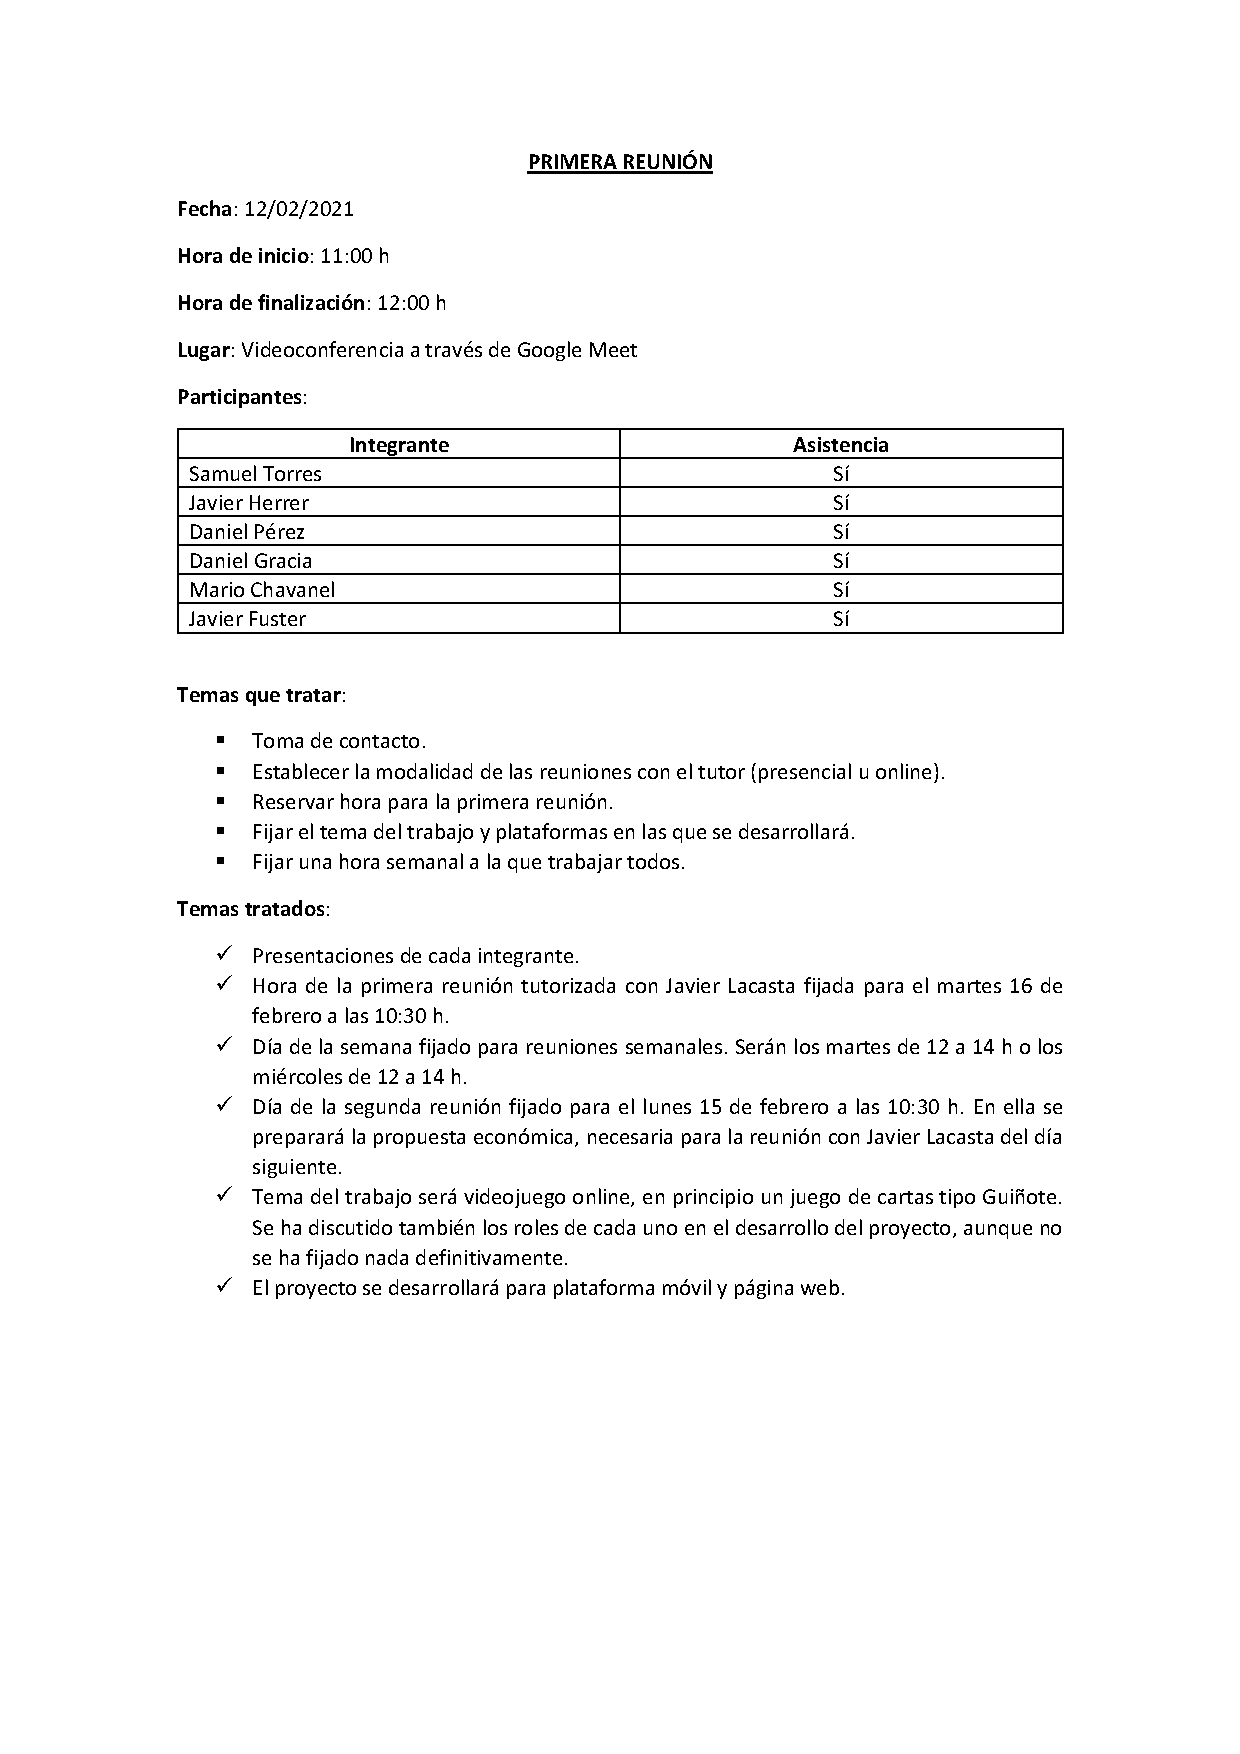
\includegraphics[width=\textwidth]{../images/actas/Acta_reunion_1.pdf}
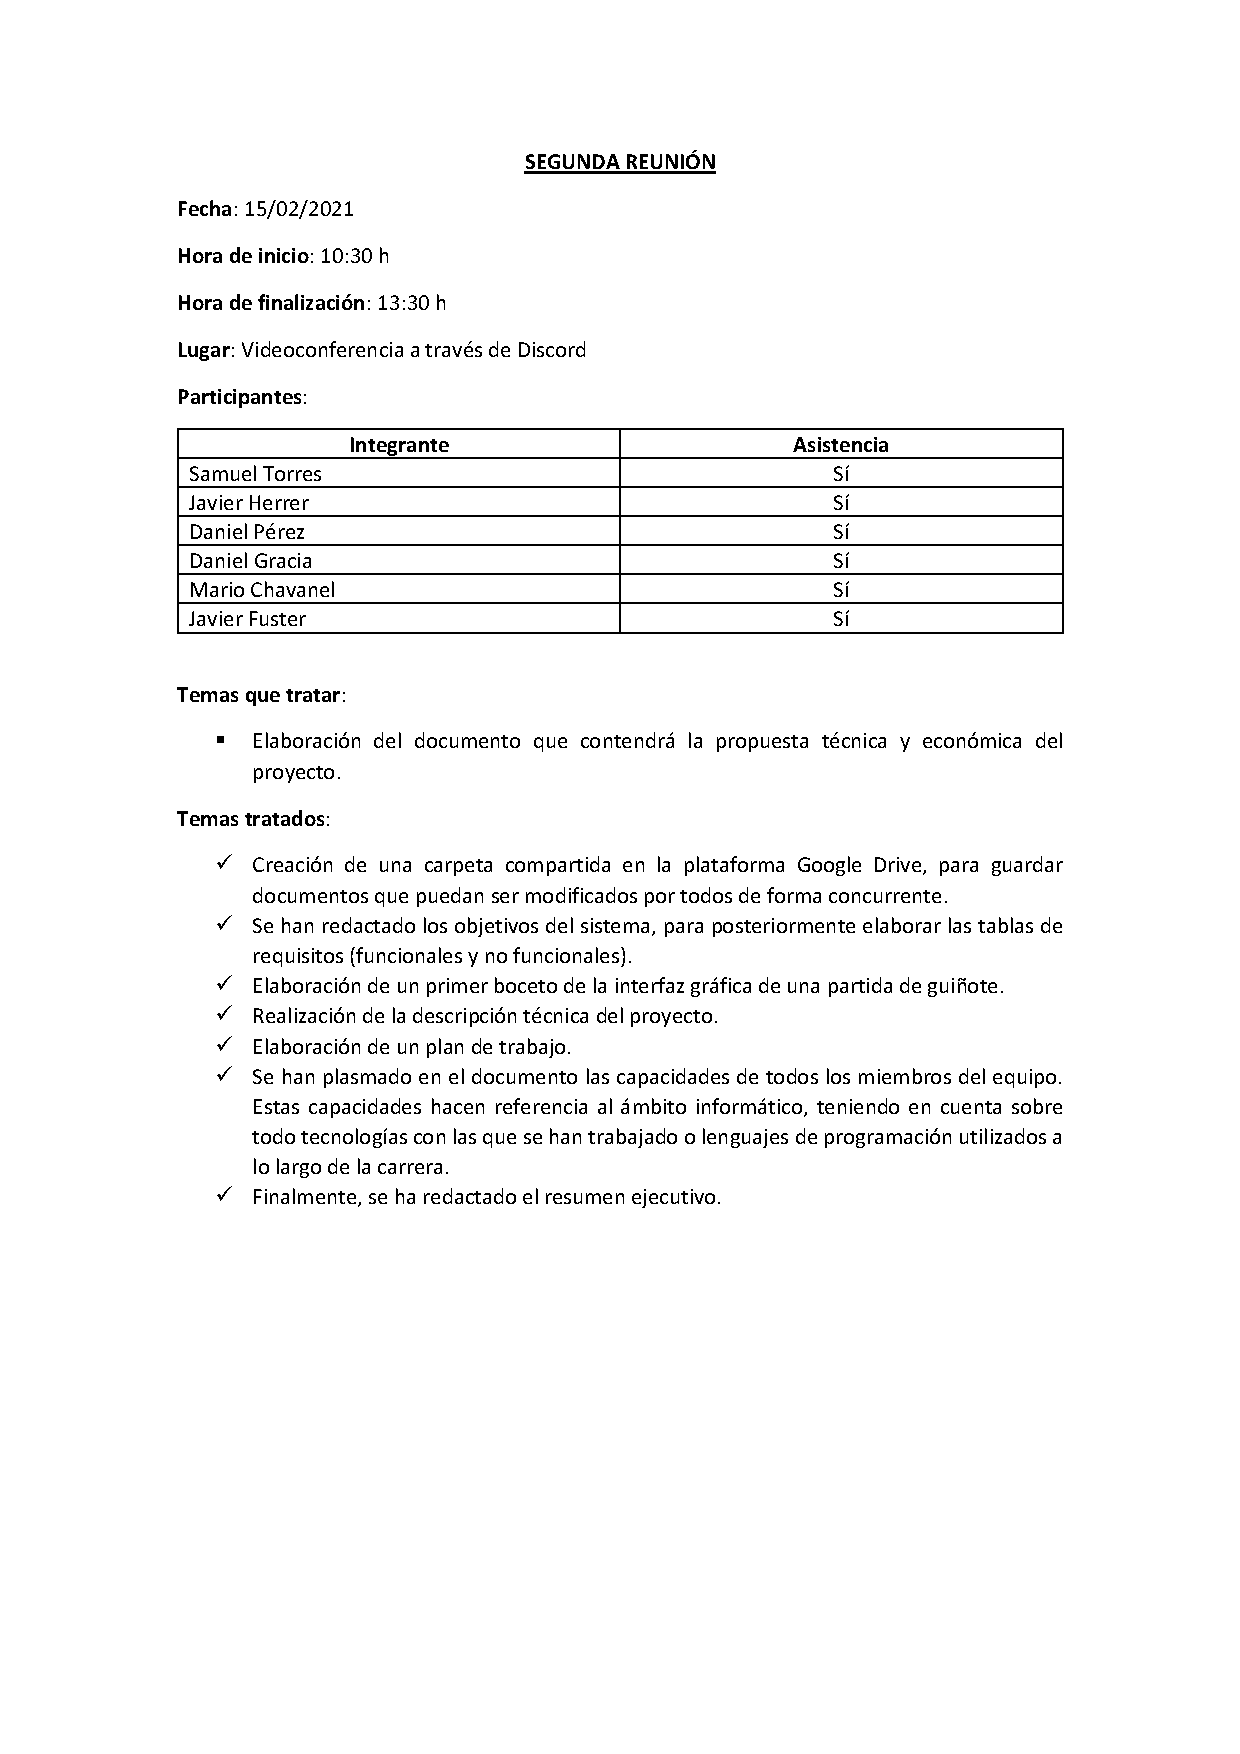
\includegraphics[width=\textwidth]{../images/actas/Acta_reunion_2.pdf}
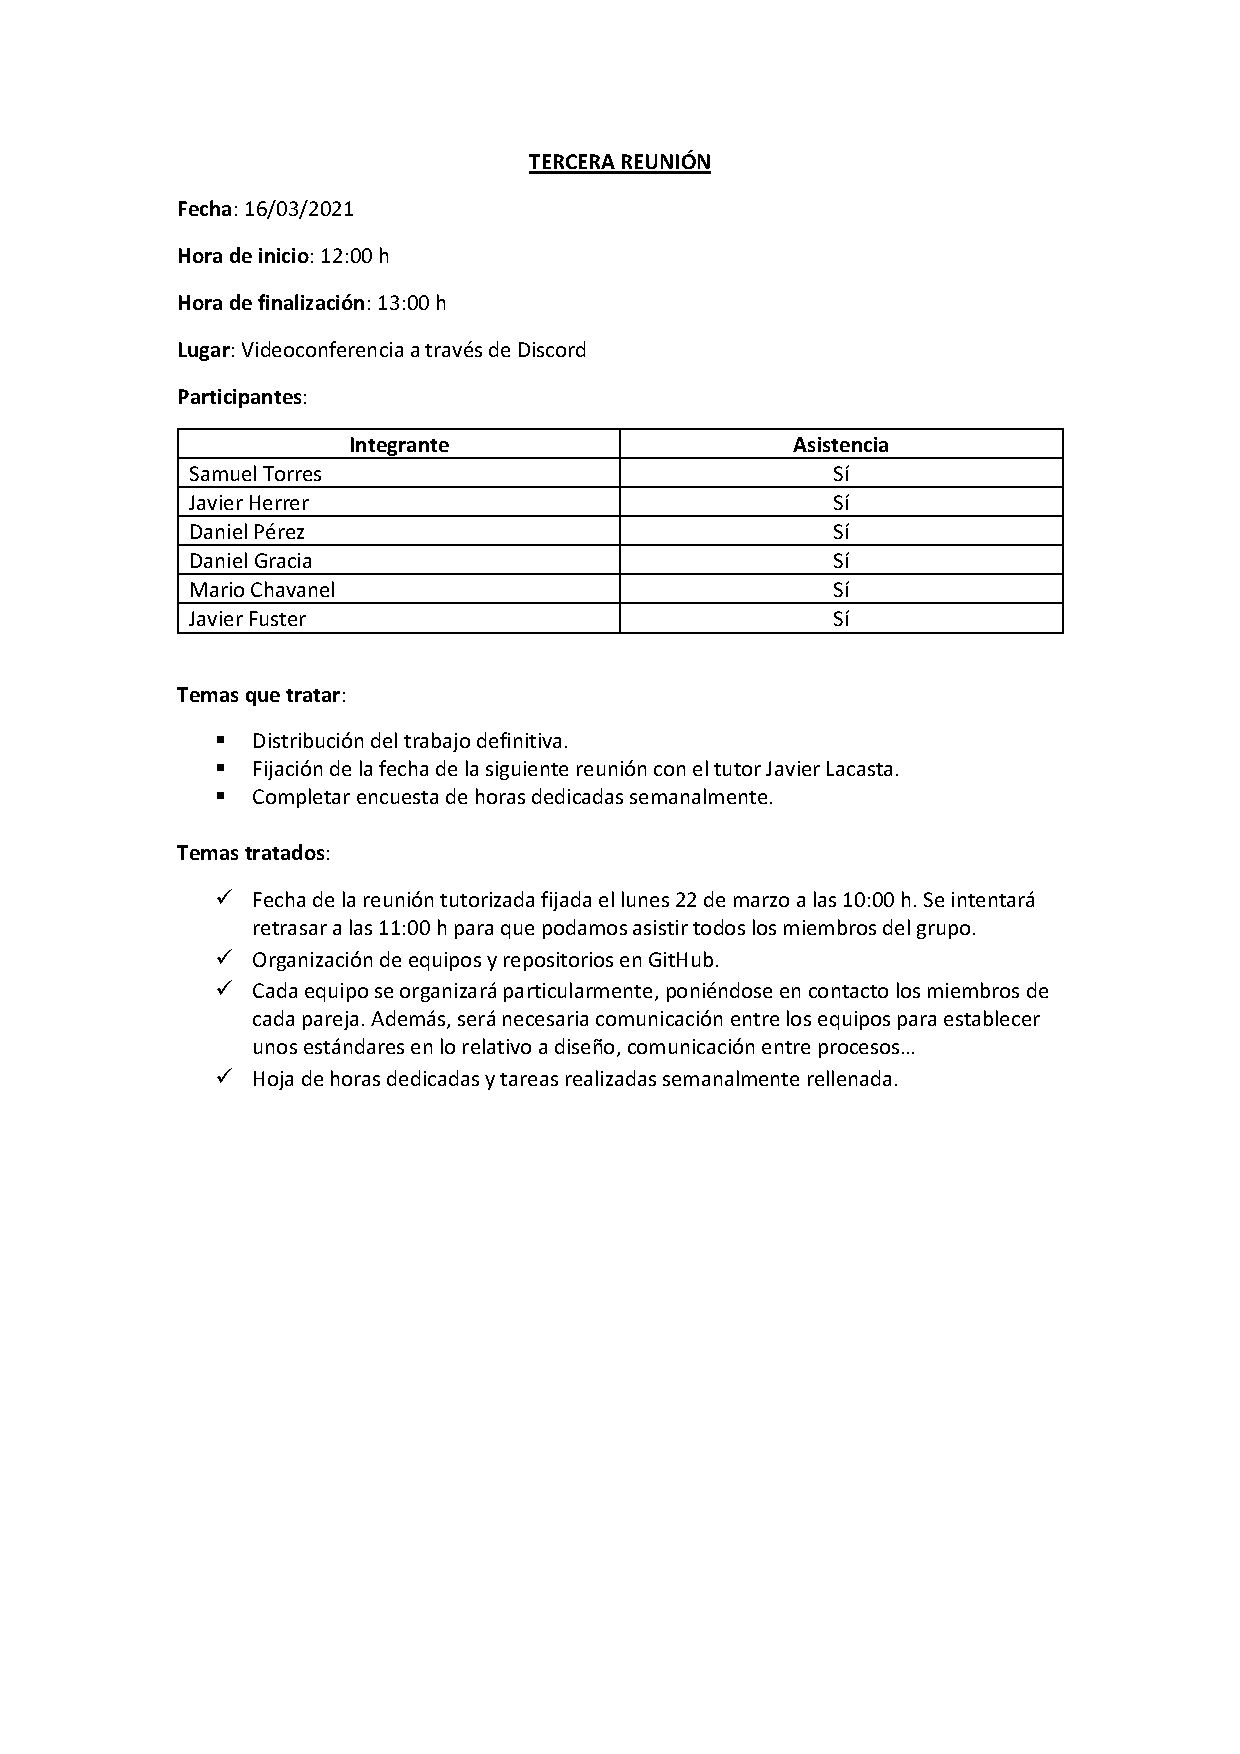
\includegraphics[width=\textwidth]{../images/actas/Acta_reunion_3.pdf}
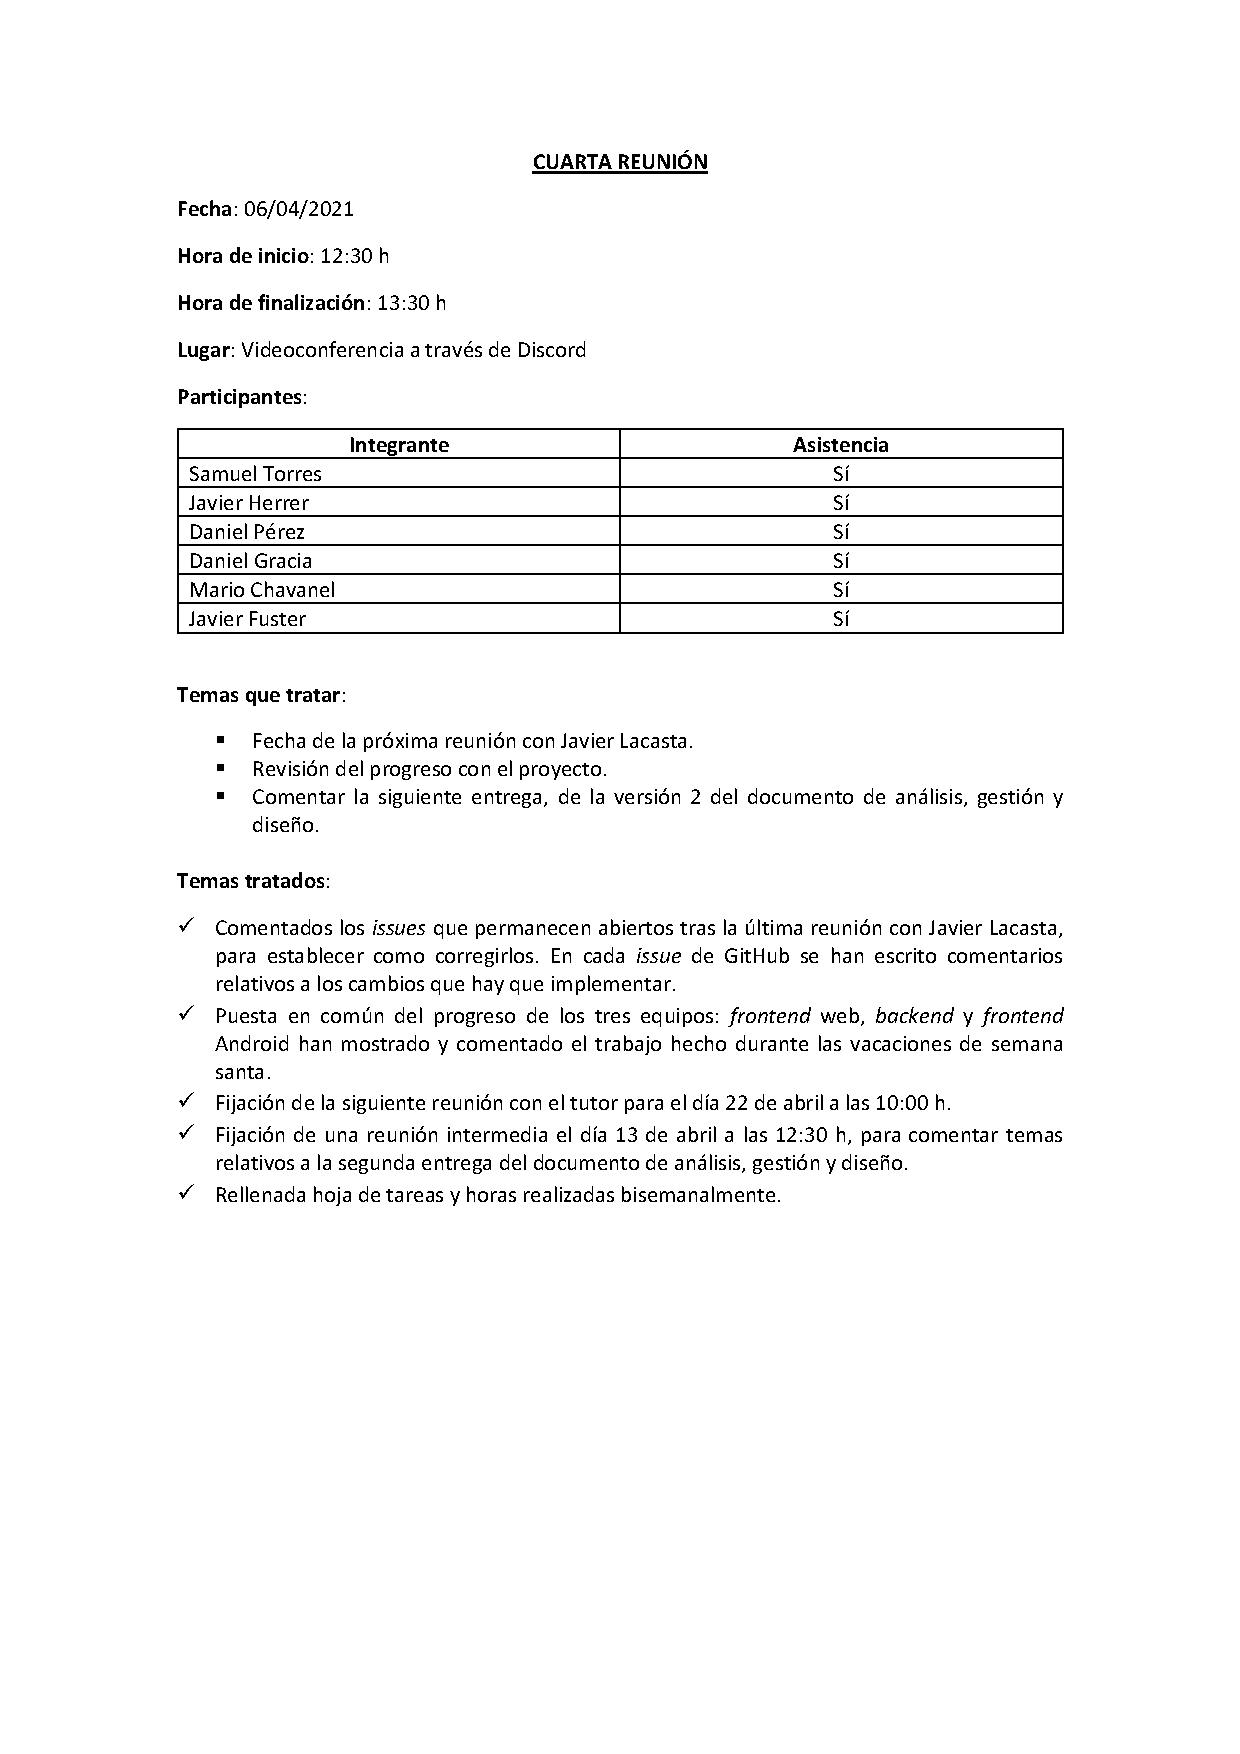
\includegraphics[width=\textwidth]{../images/actas/Acta_reunion_4.pdf}
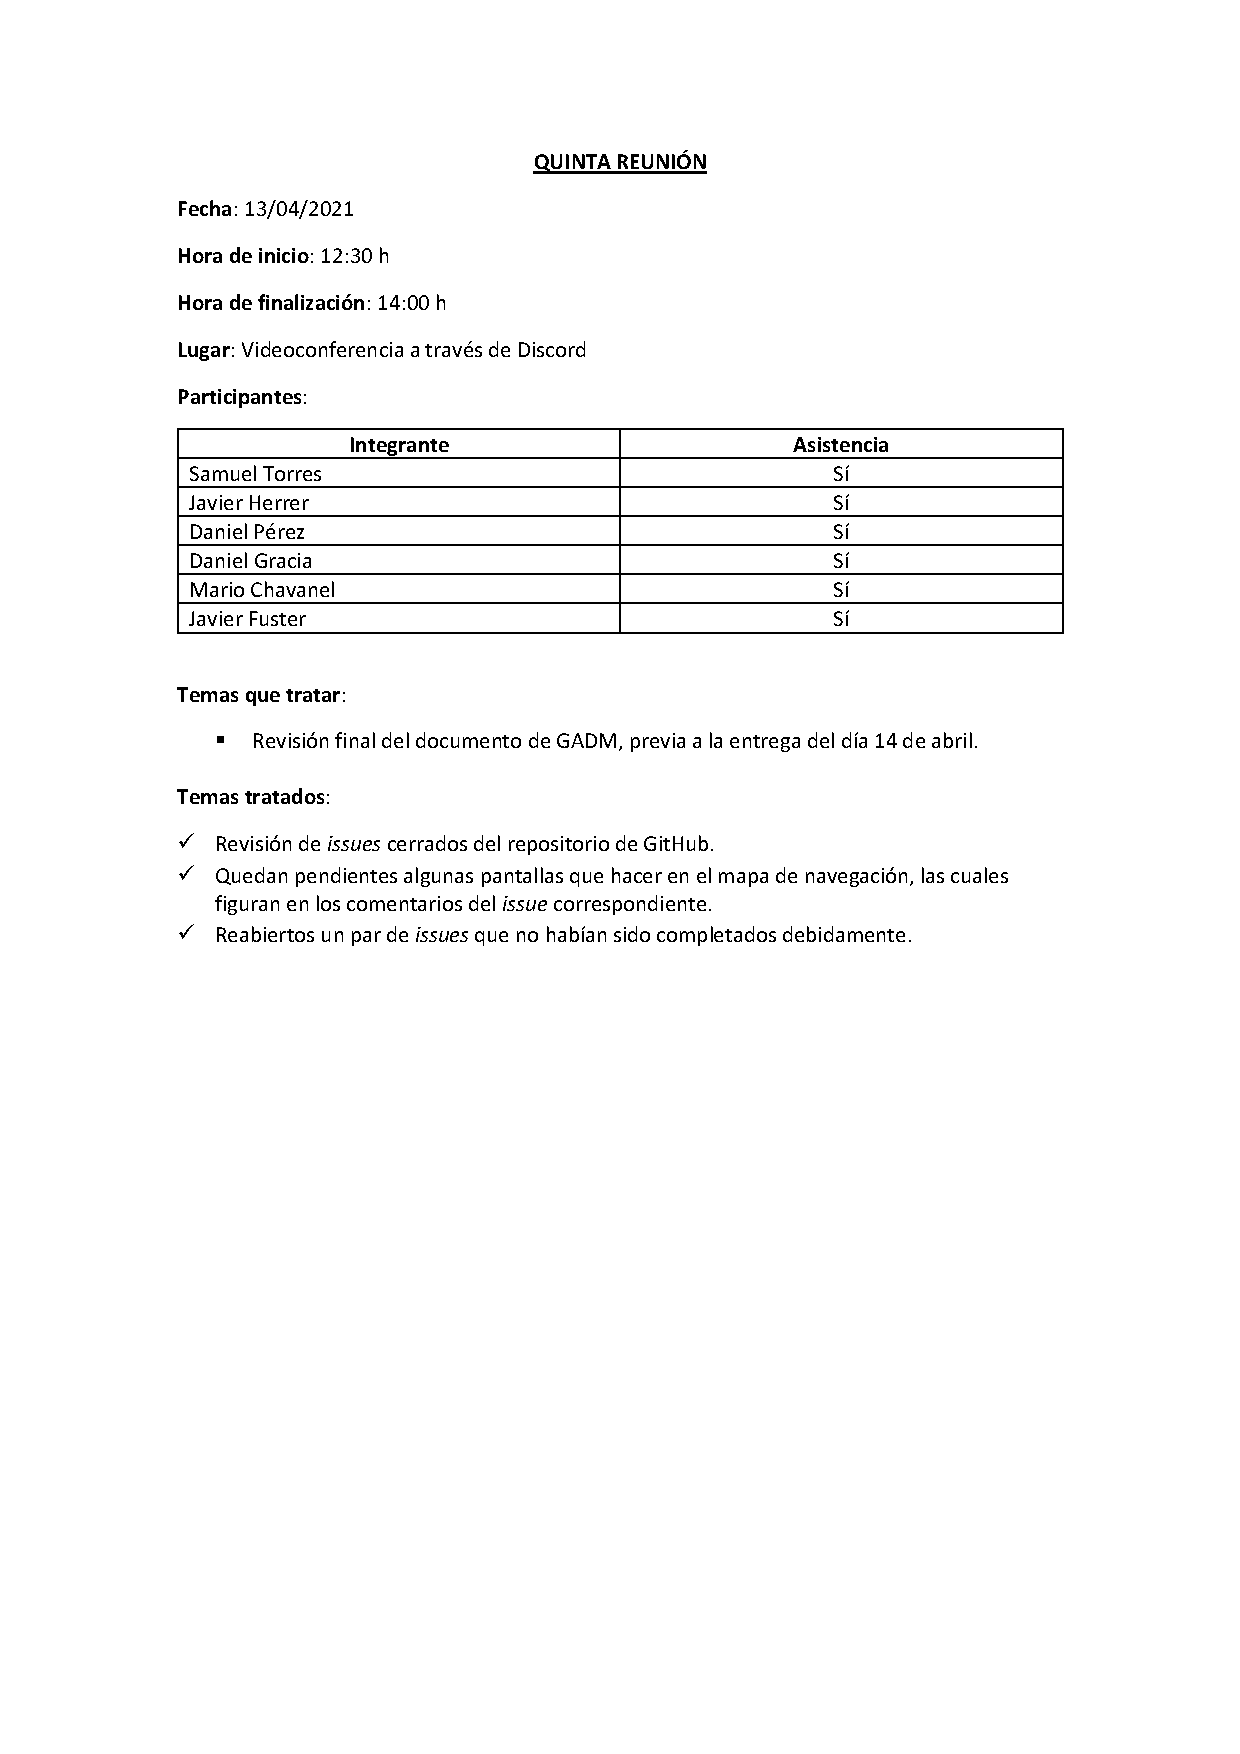
\includegraphics[width=\textwidth]{../images/actas/Acta_reunion_5.pdf}
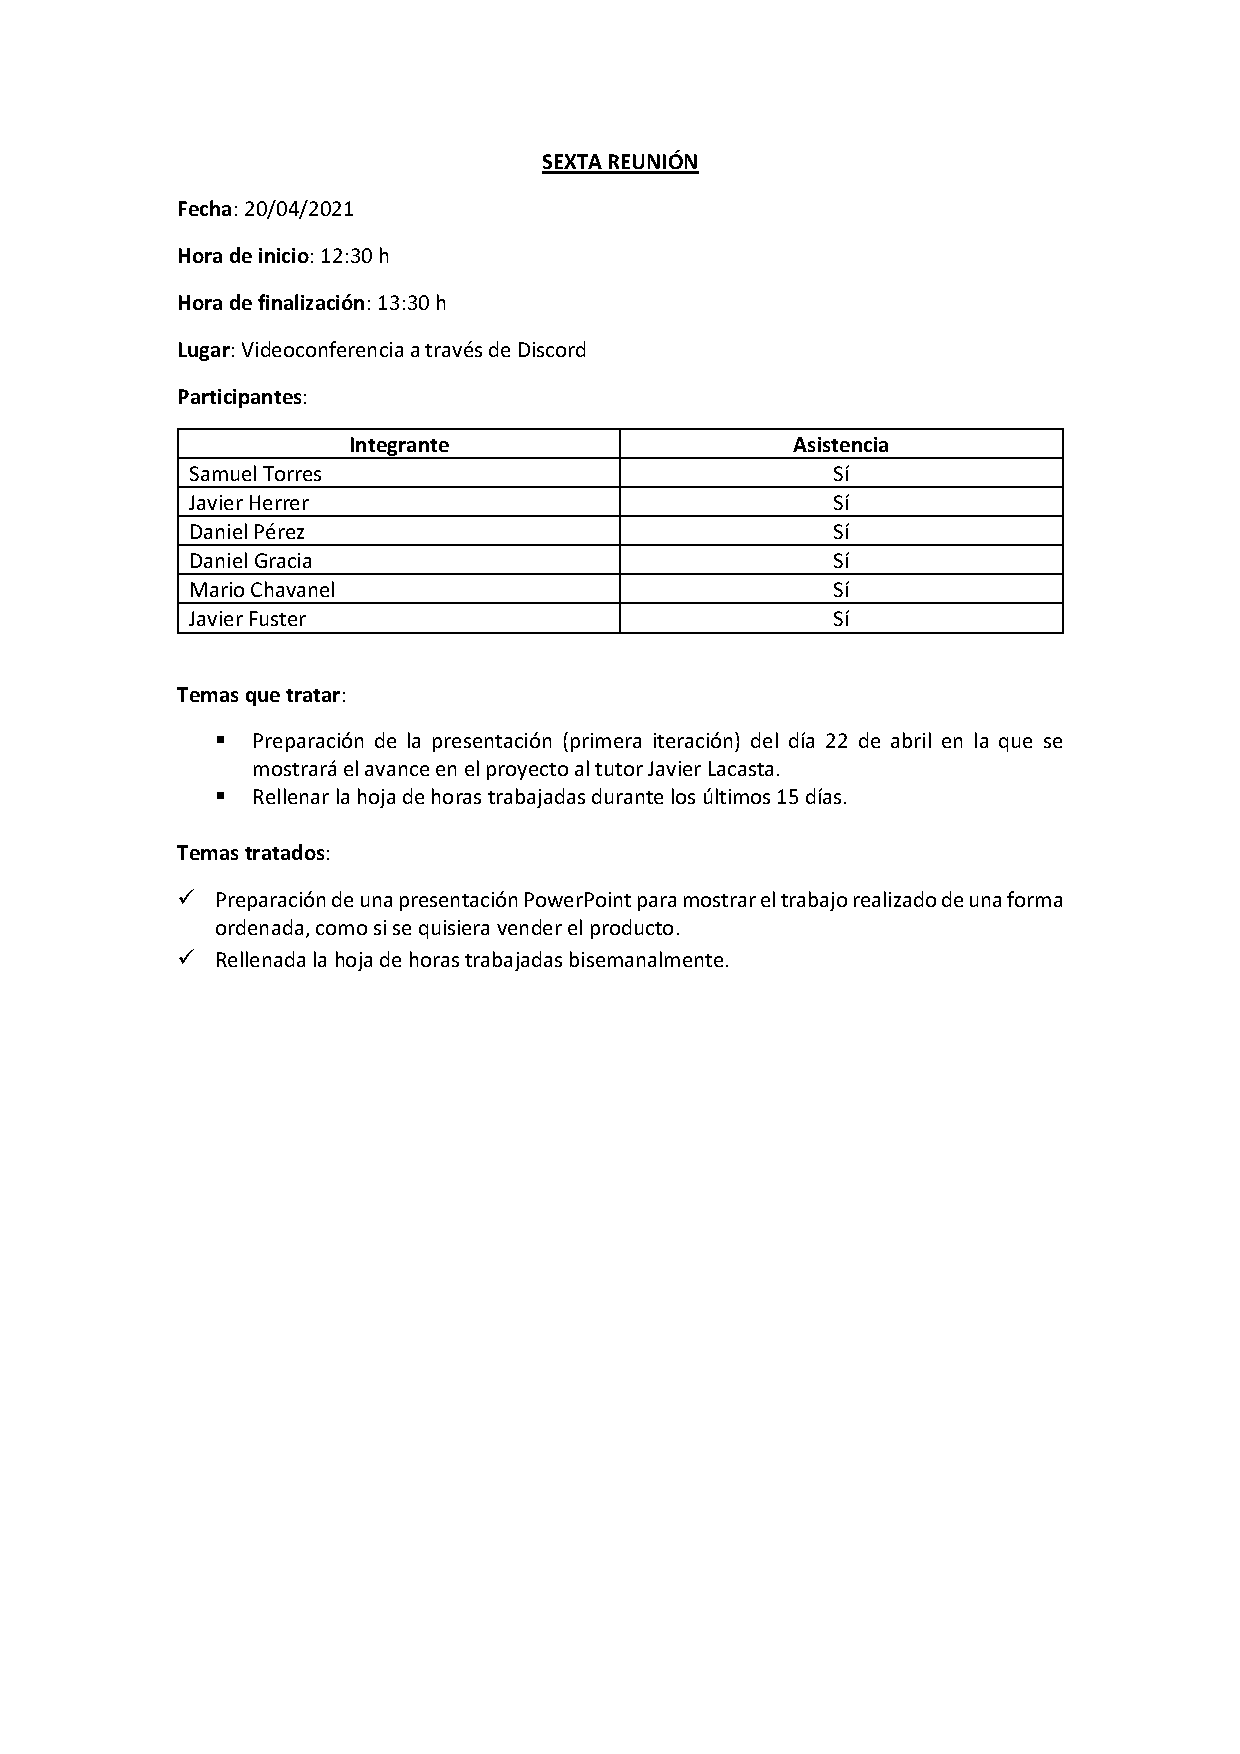
\includegraphics[width=\textwidth]{../images/actas/Acta_reunion_6.pdf}
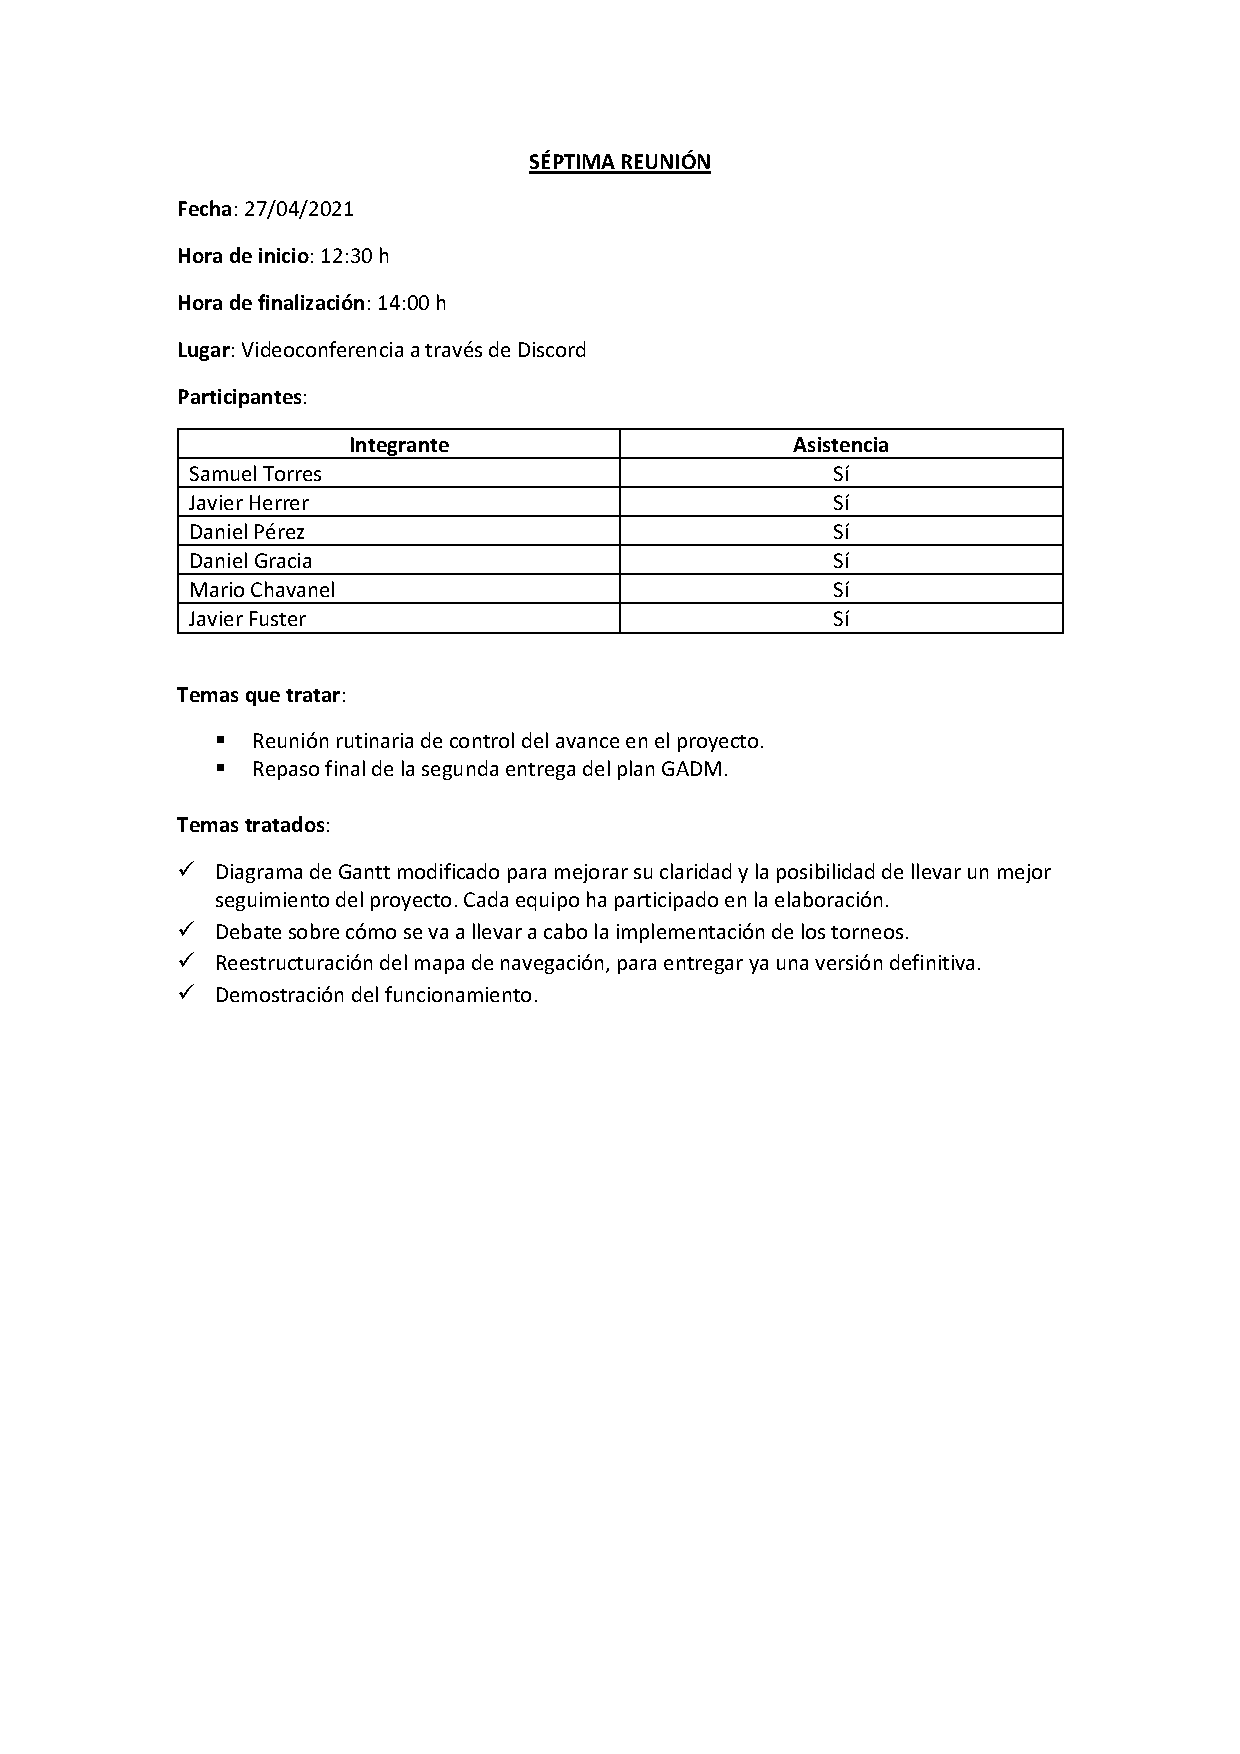
\includegraphics[width=\textwidth]{../images/actas/Acta_reunion_7.pdf}
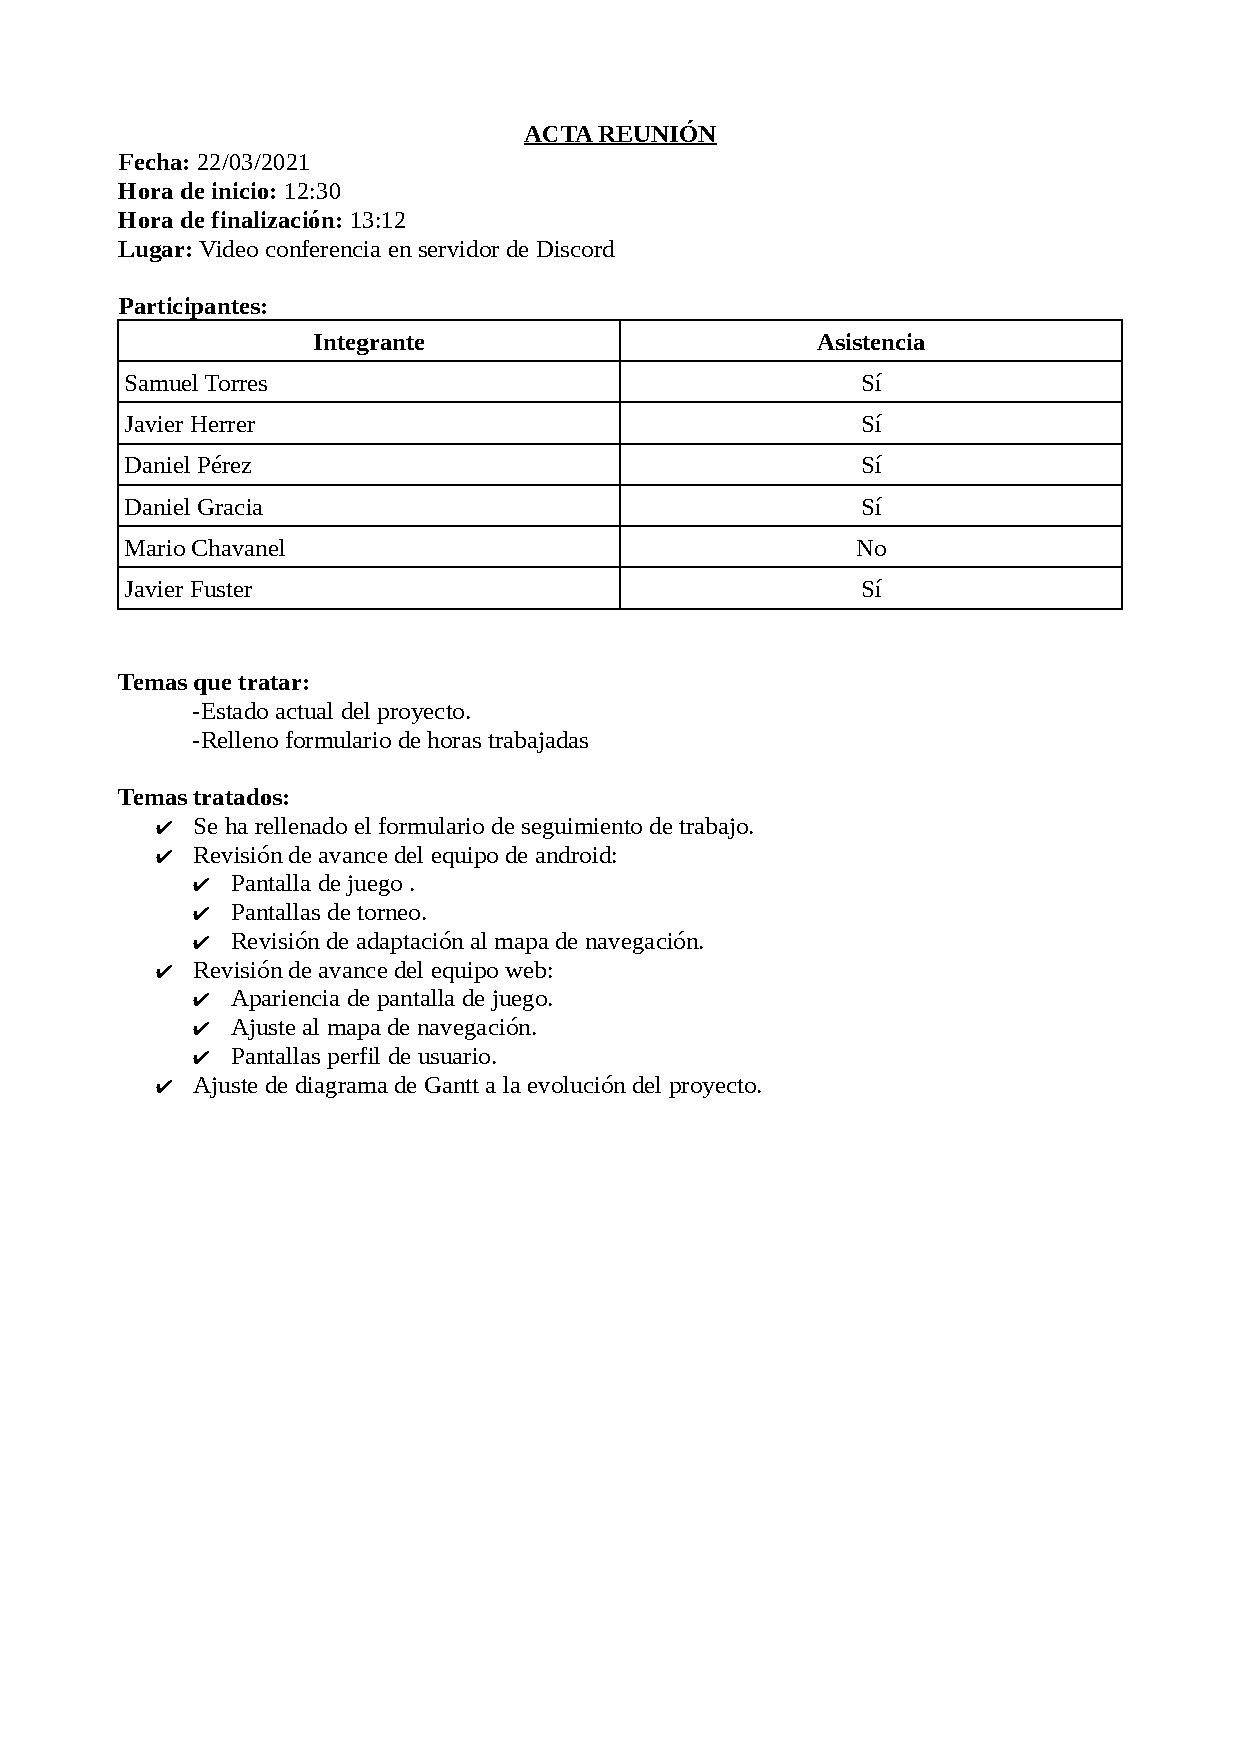
\includegraphics[width=\textwidth]{../images/actas/Acta_reunion_8.pdf}
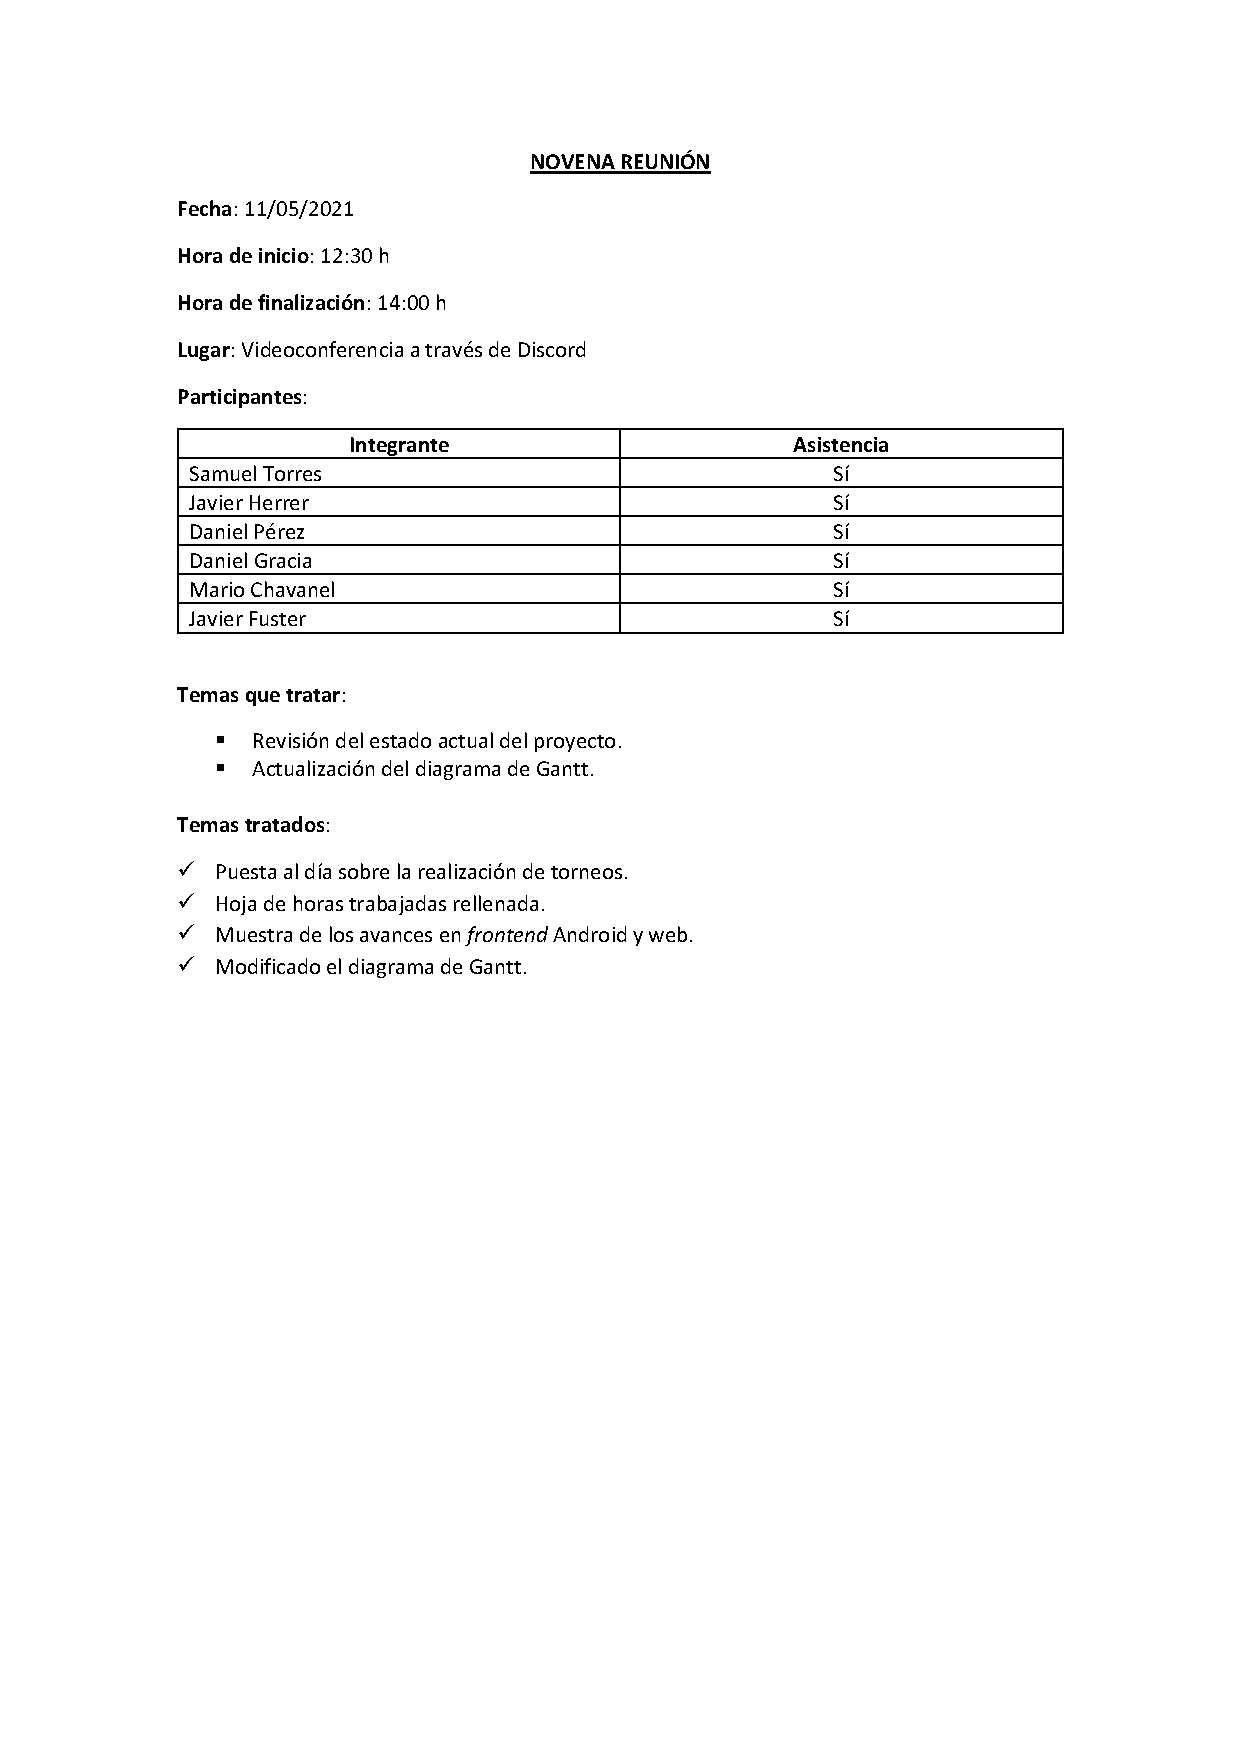
\includegraphics[width=\textwidth]{../images/actas/Acta_reunion_9.pdf}
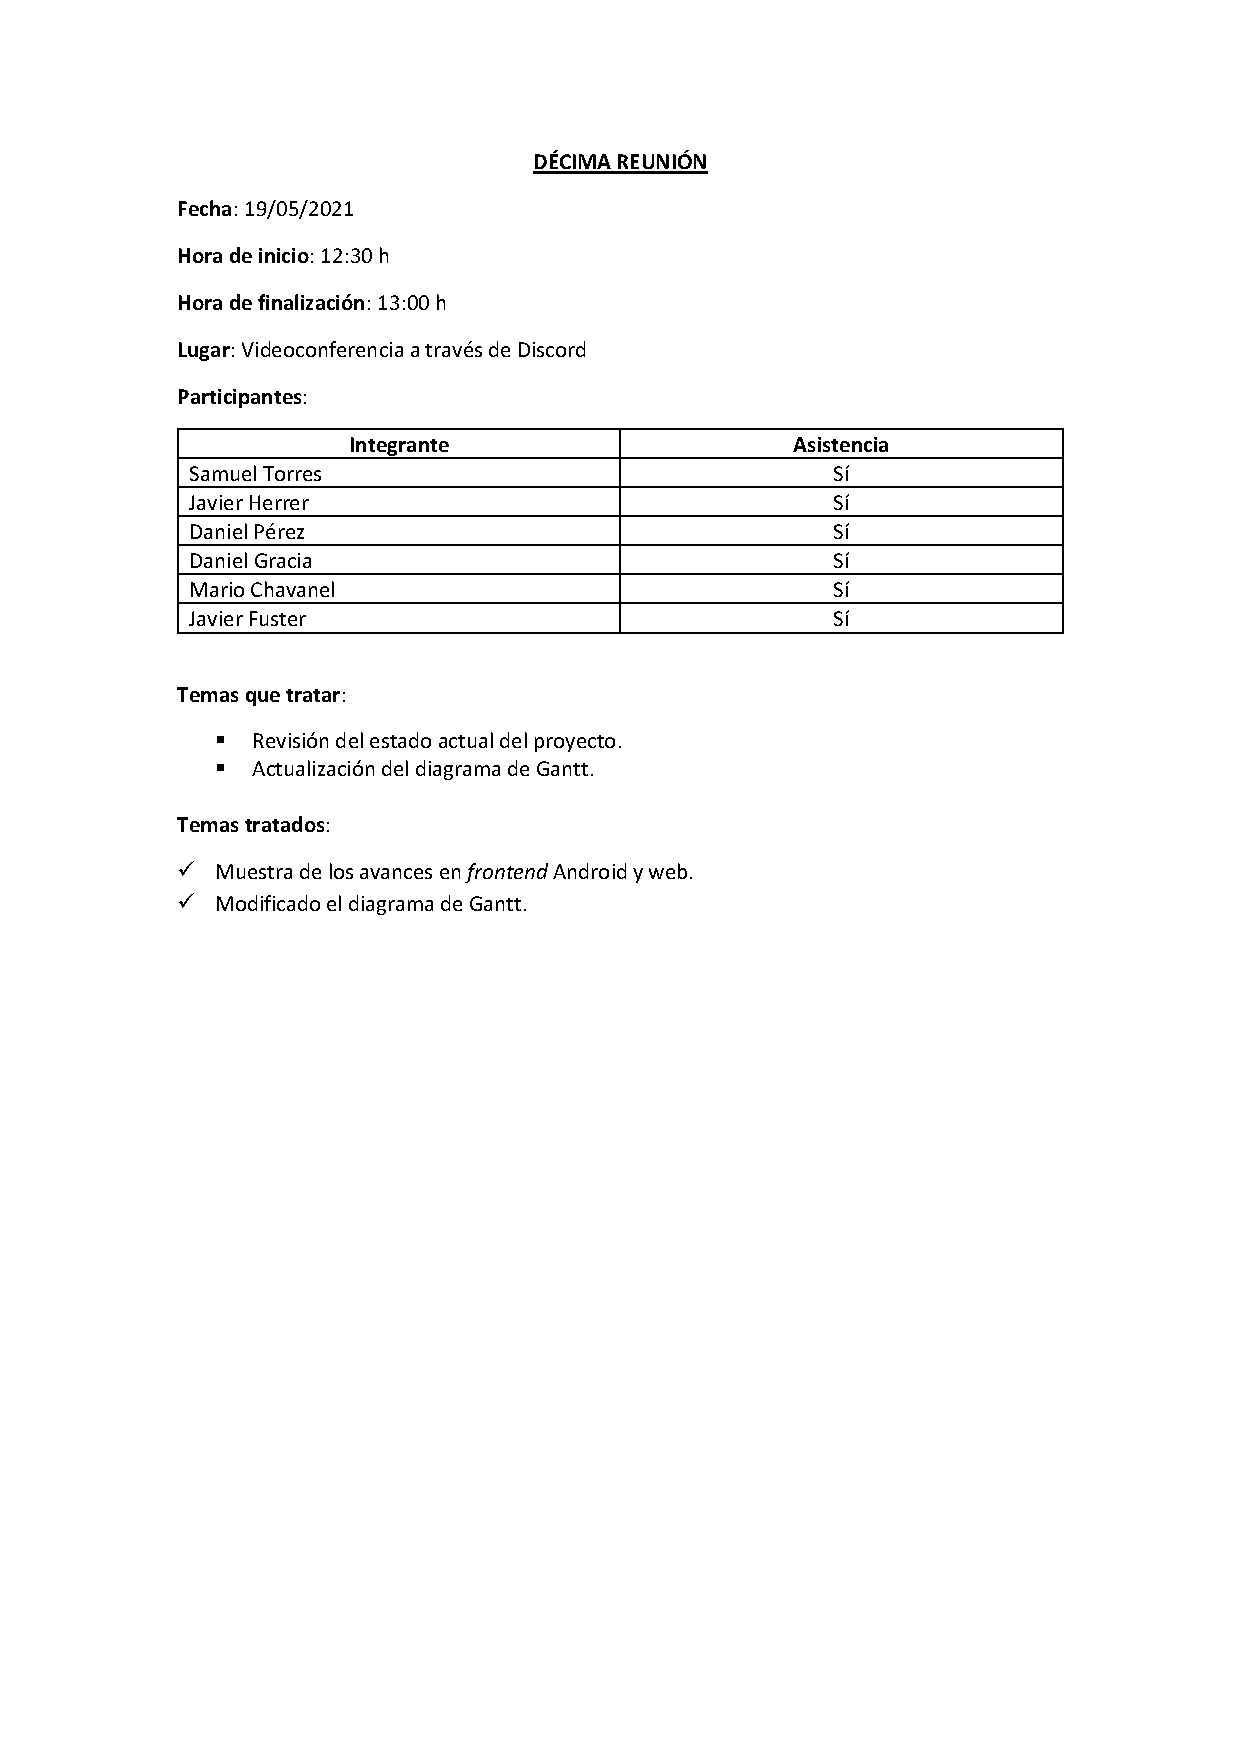
\includegraphics[width=\textwidth]{../images/actas/Acta_reunion_10.pdf}
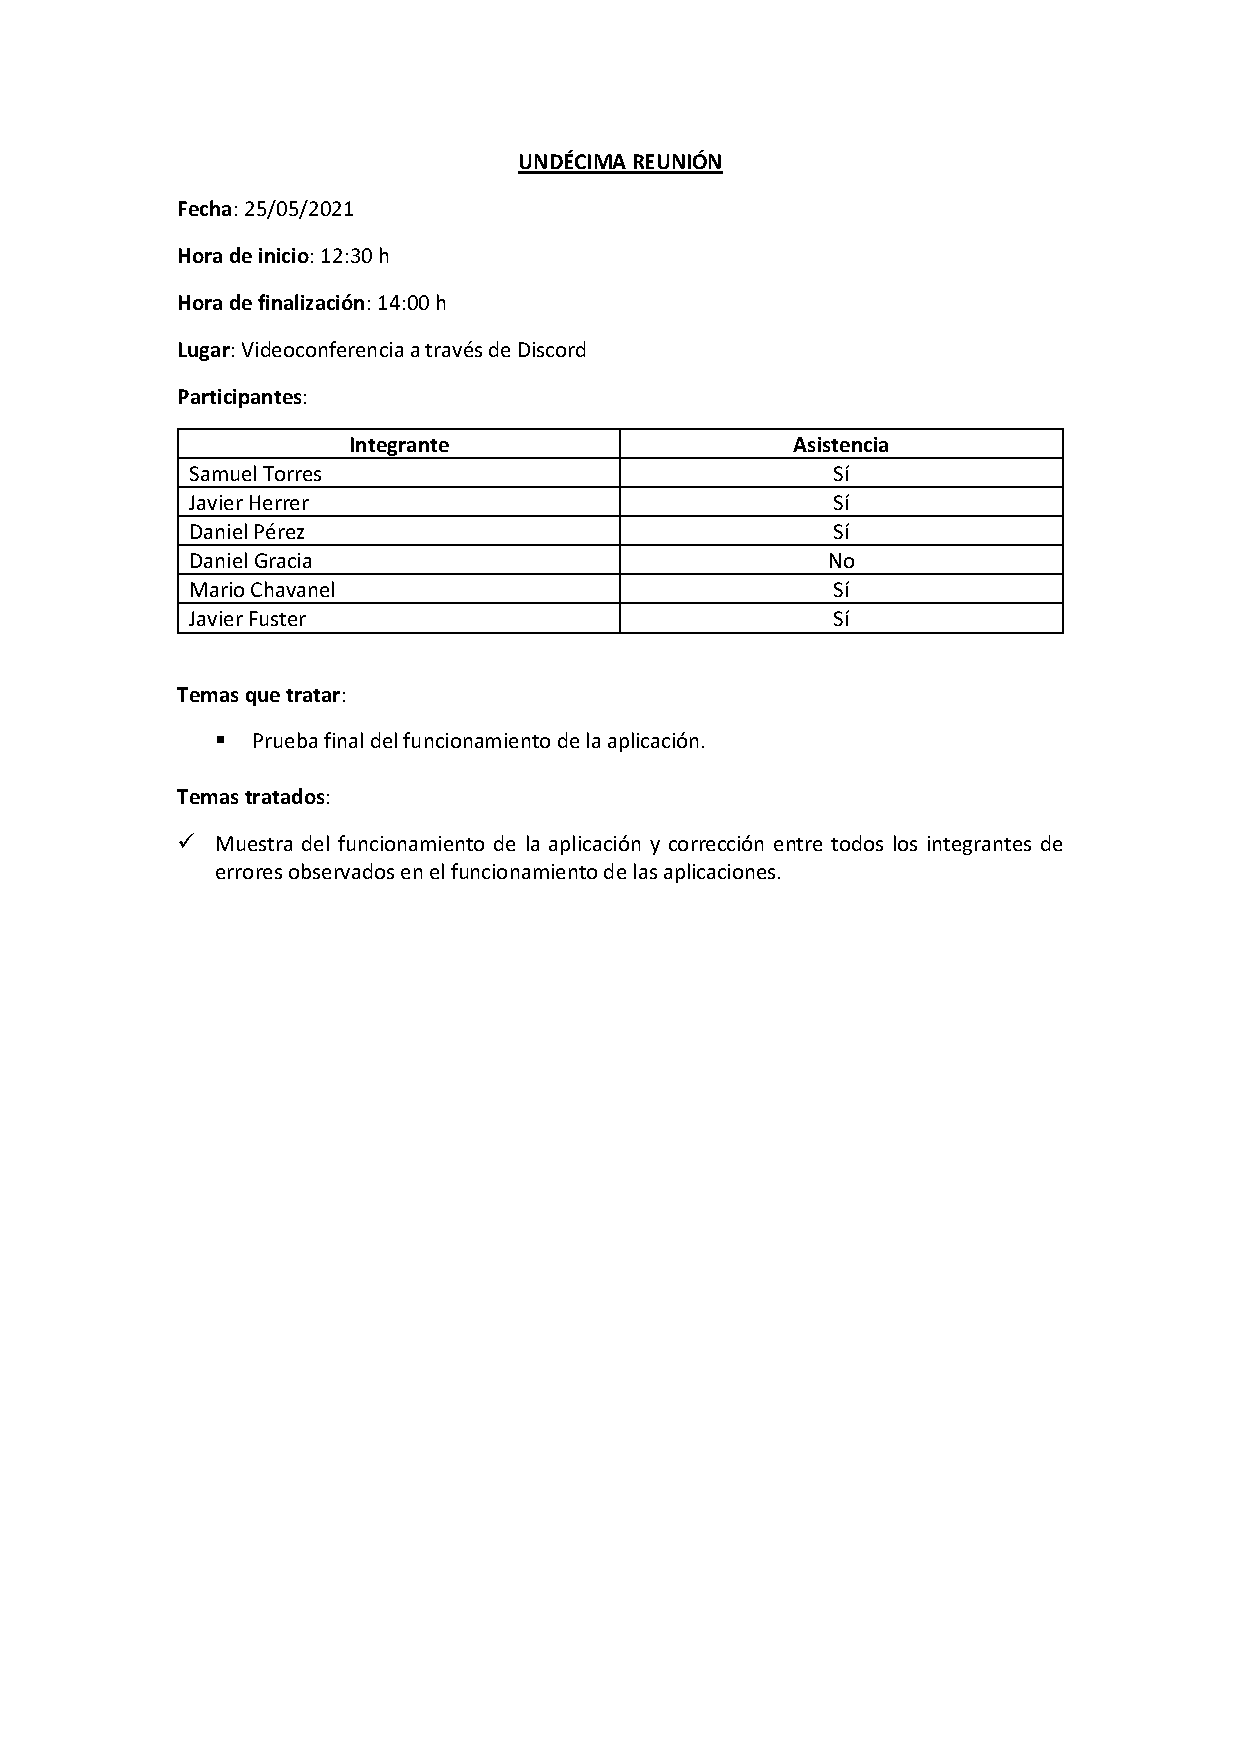
\includegraphics[width=\textwidth]{../images/actas/Acta_reunion_11.pdf}
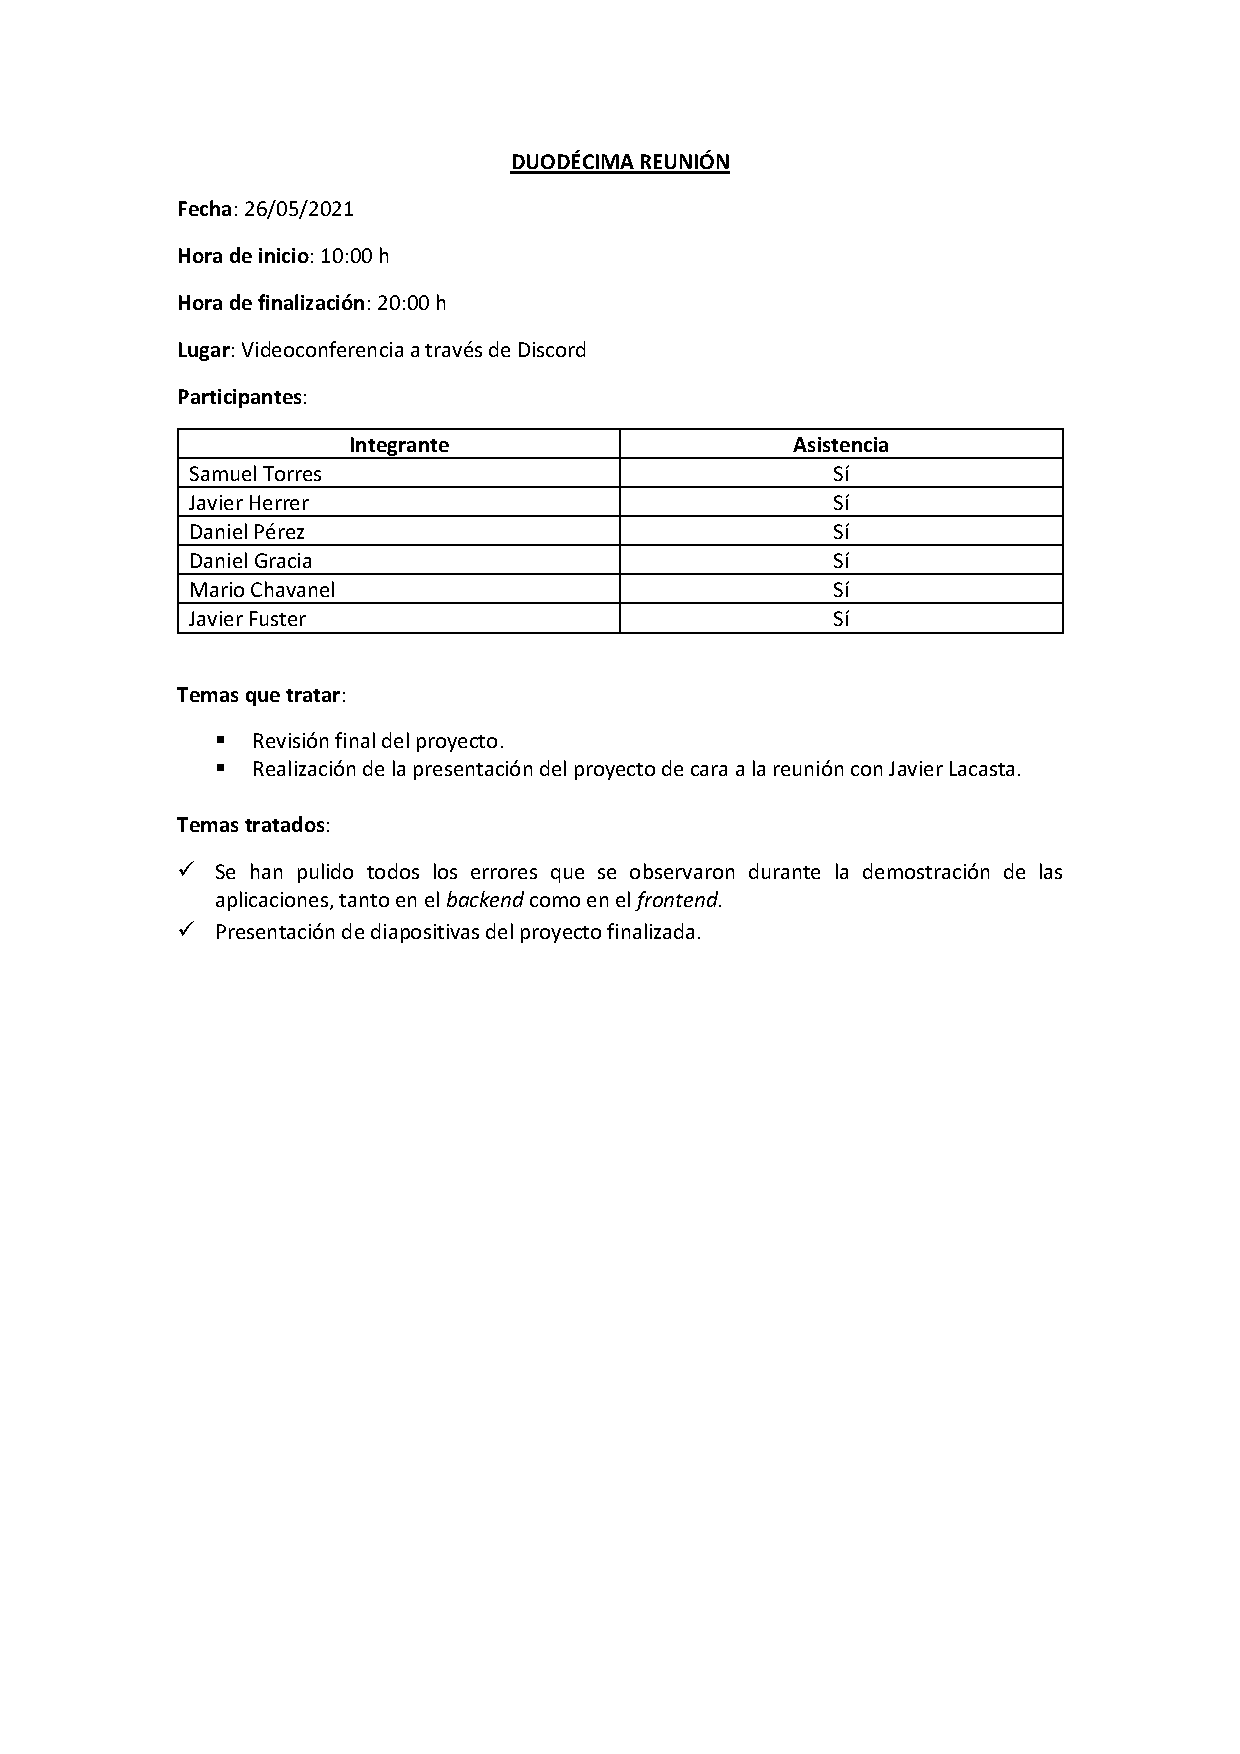
\includegraphics[width=\textwidth]{../images/actas/Acta_reunion_12.pdf}

\subsection*{Reuniones tutorizadas}
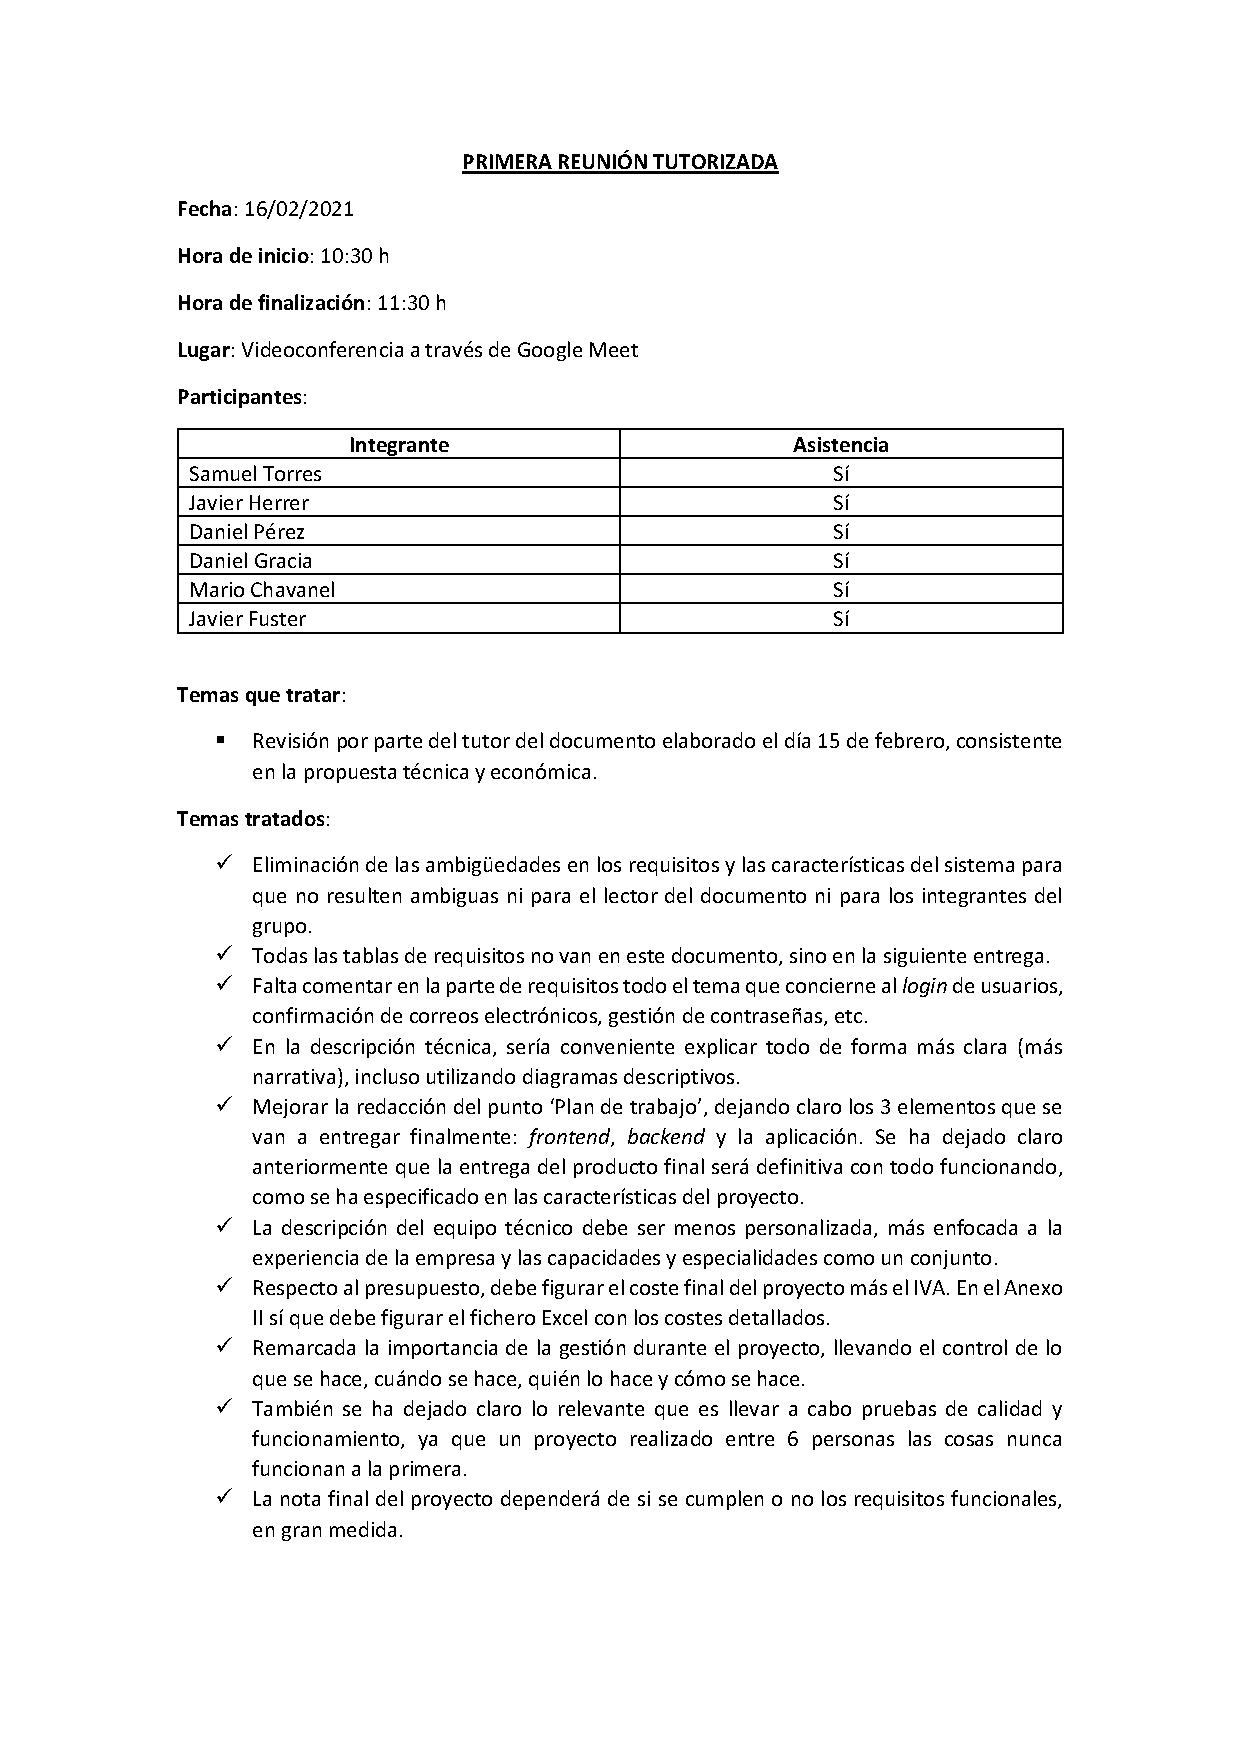
\includegraphics[width=\textwidth]{../images/actas/Acta_reunion_tutorizada_1.pdf}


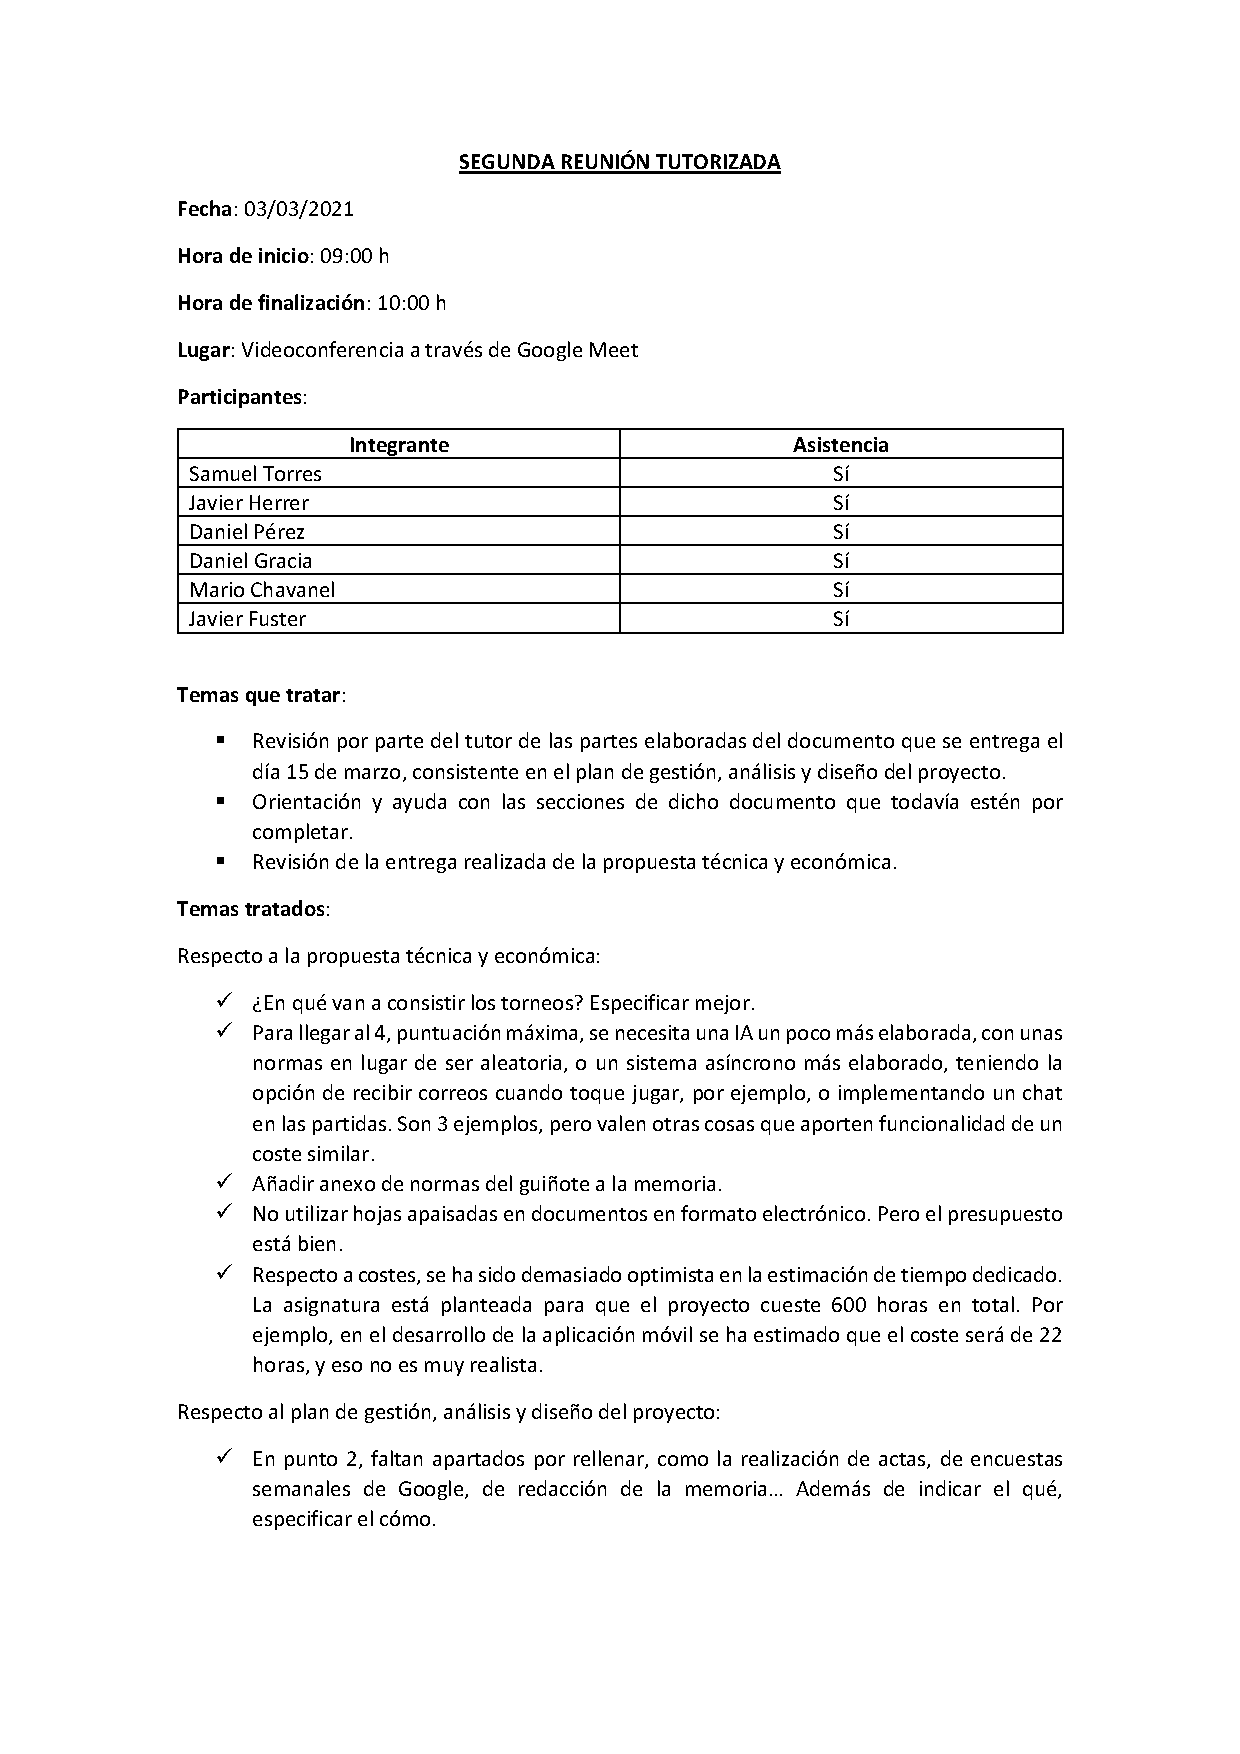
\includegraphics[width=\textwidth]{../images/actas/Acta_reunion_tutorizada_2.pdf}
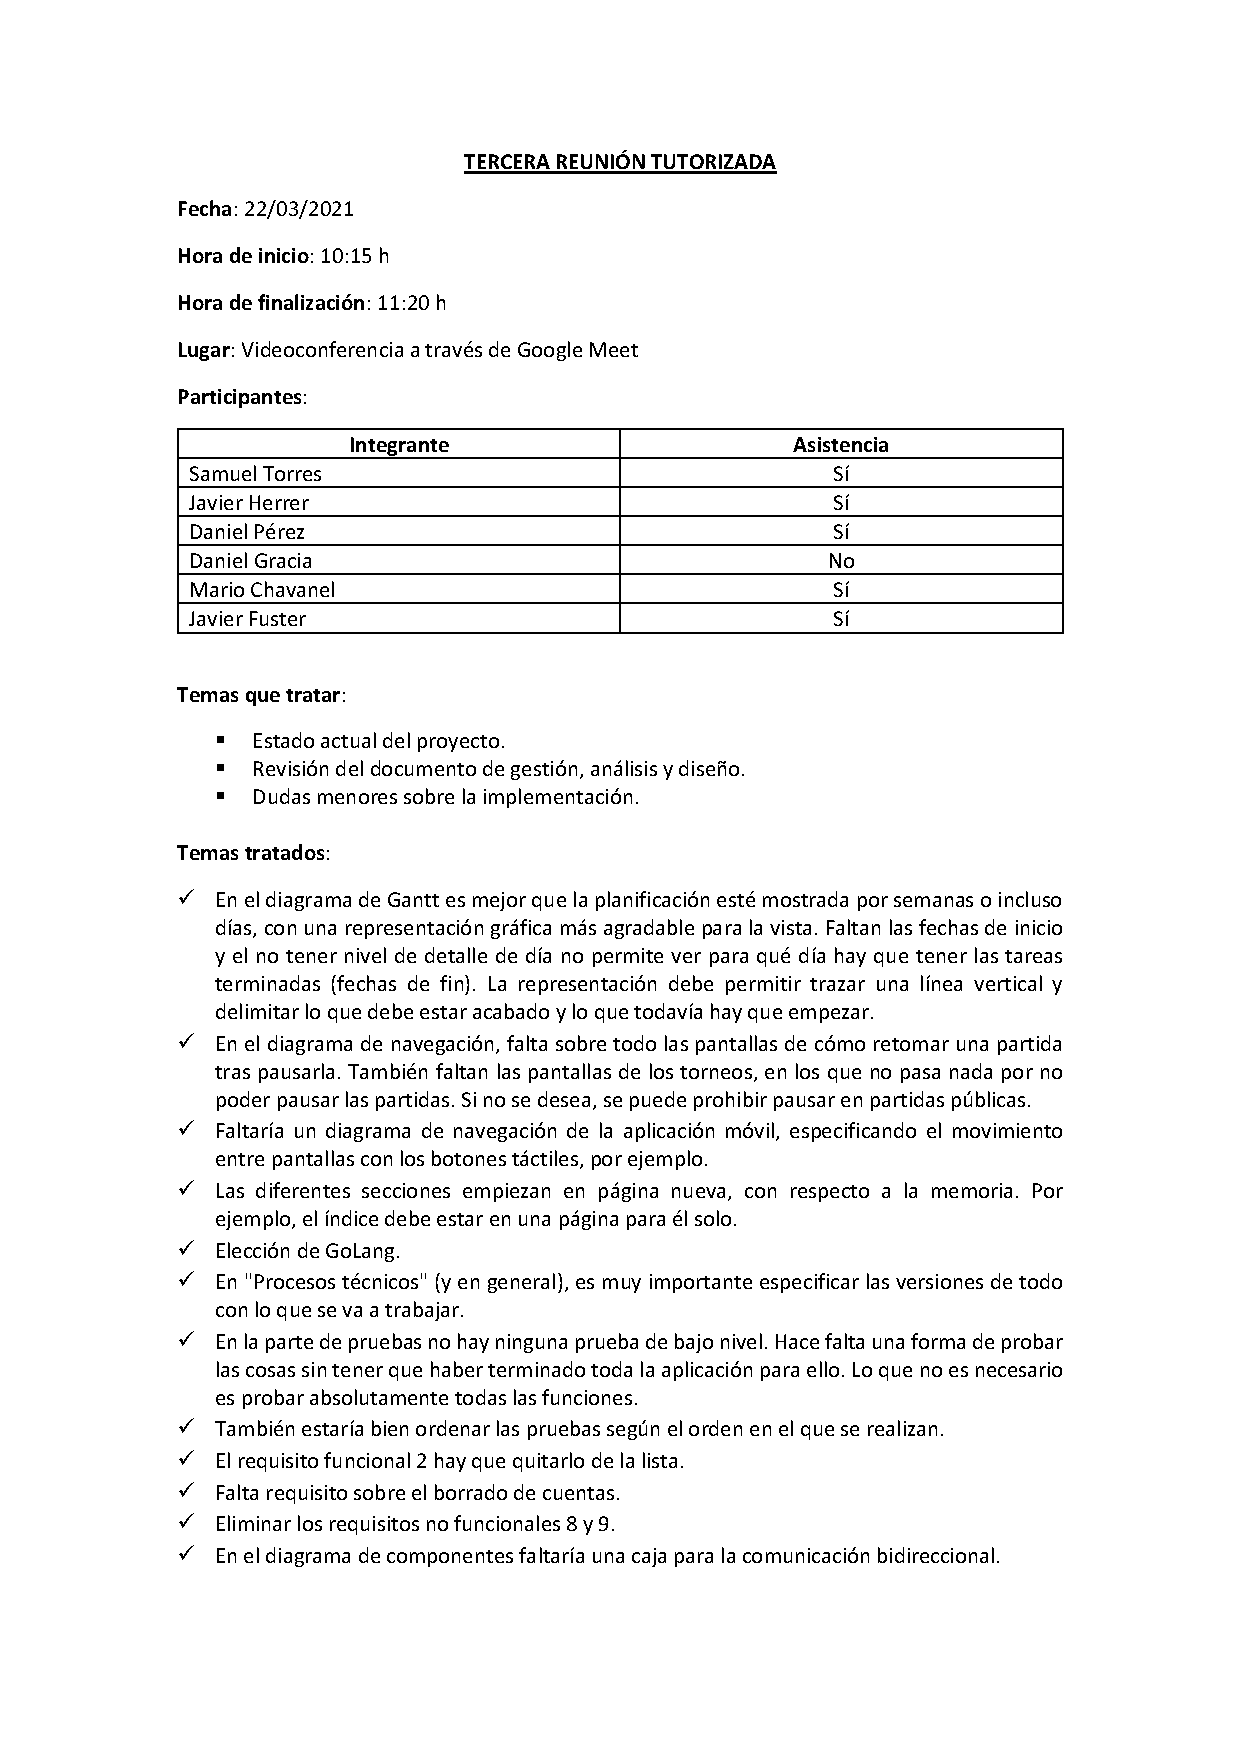
\includegraphics[width=\textwidth]{../images/actas/Acta_reunion_tutorizada_3.pdf}
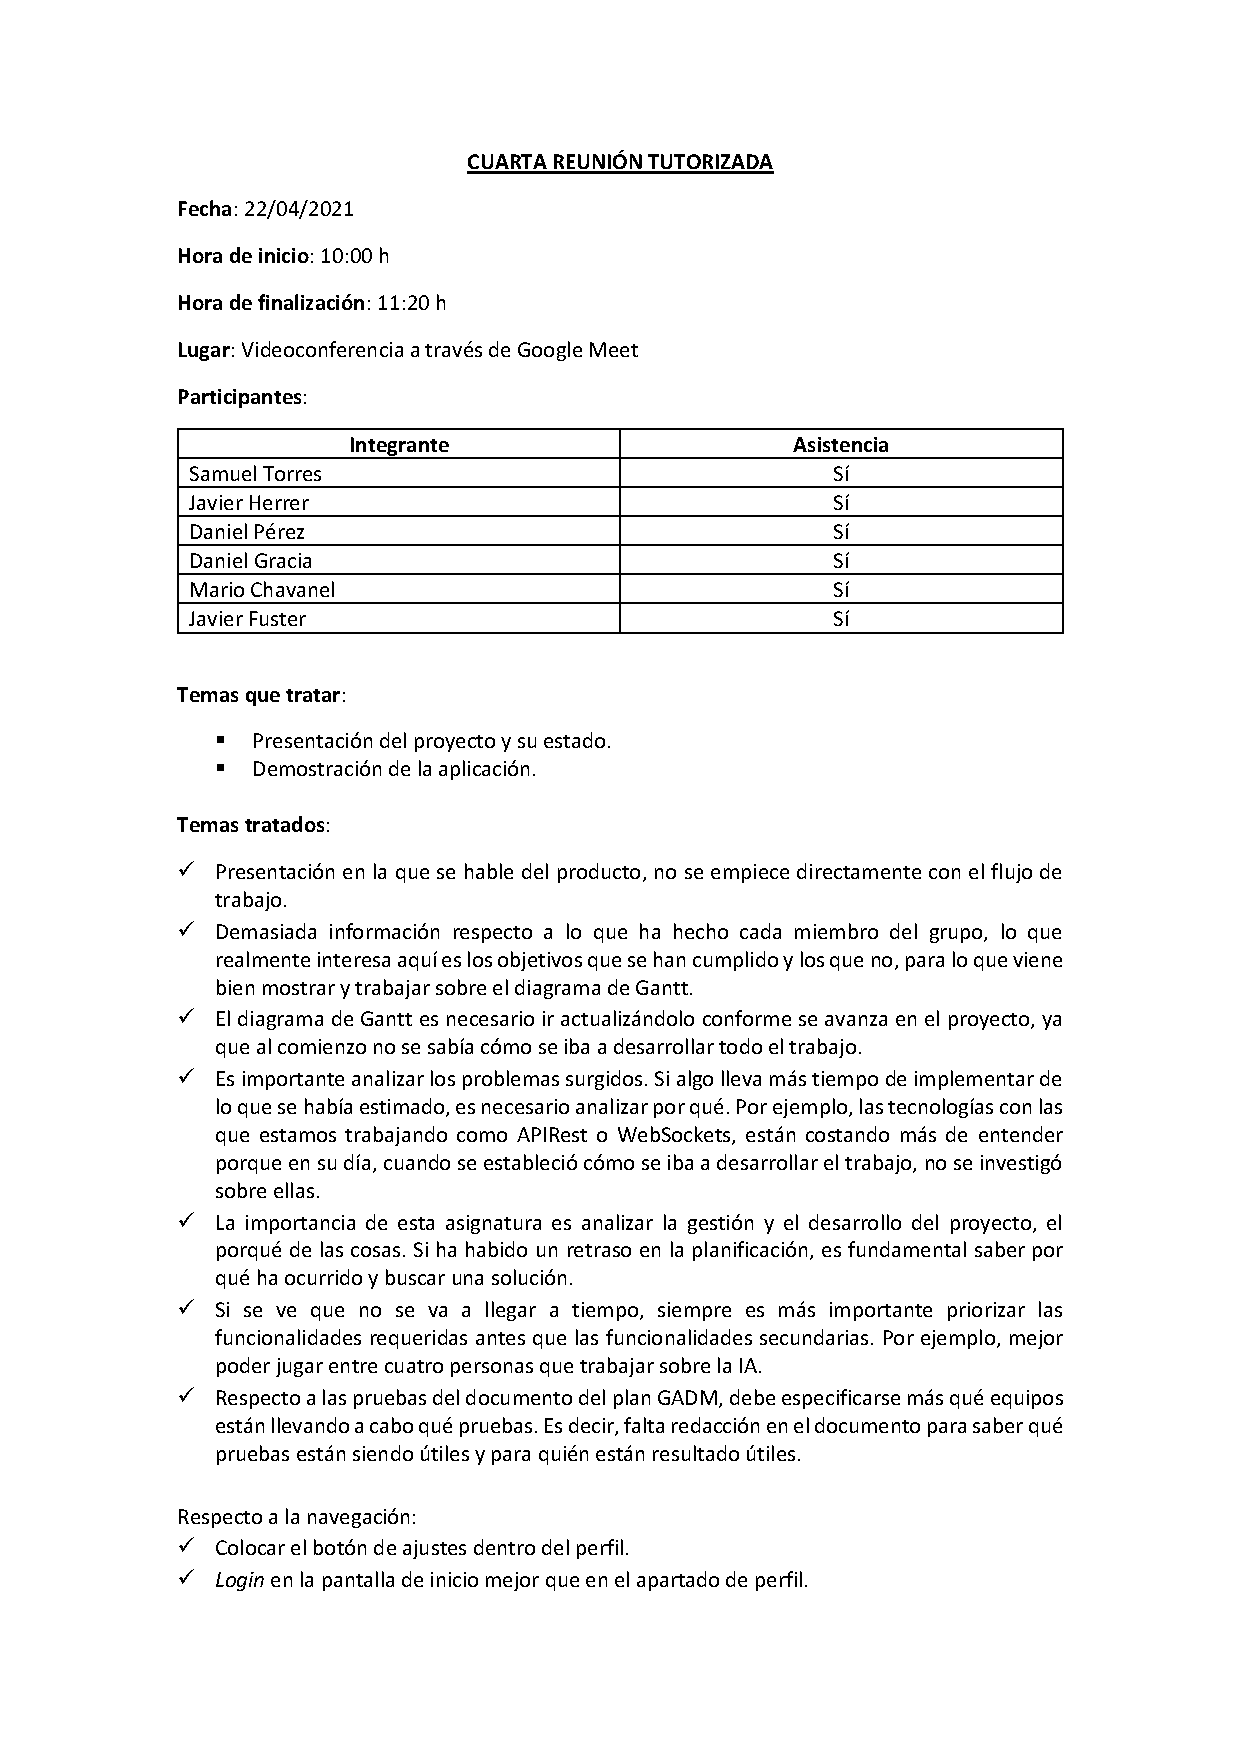
\includegraphics[width=\textwidth]{../images/actas/Acta_reunion_tutorizada_4.pdf}
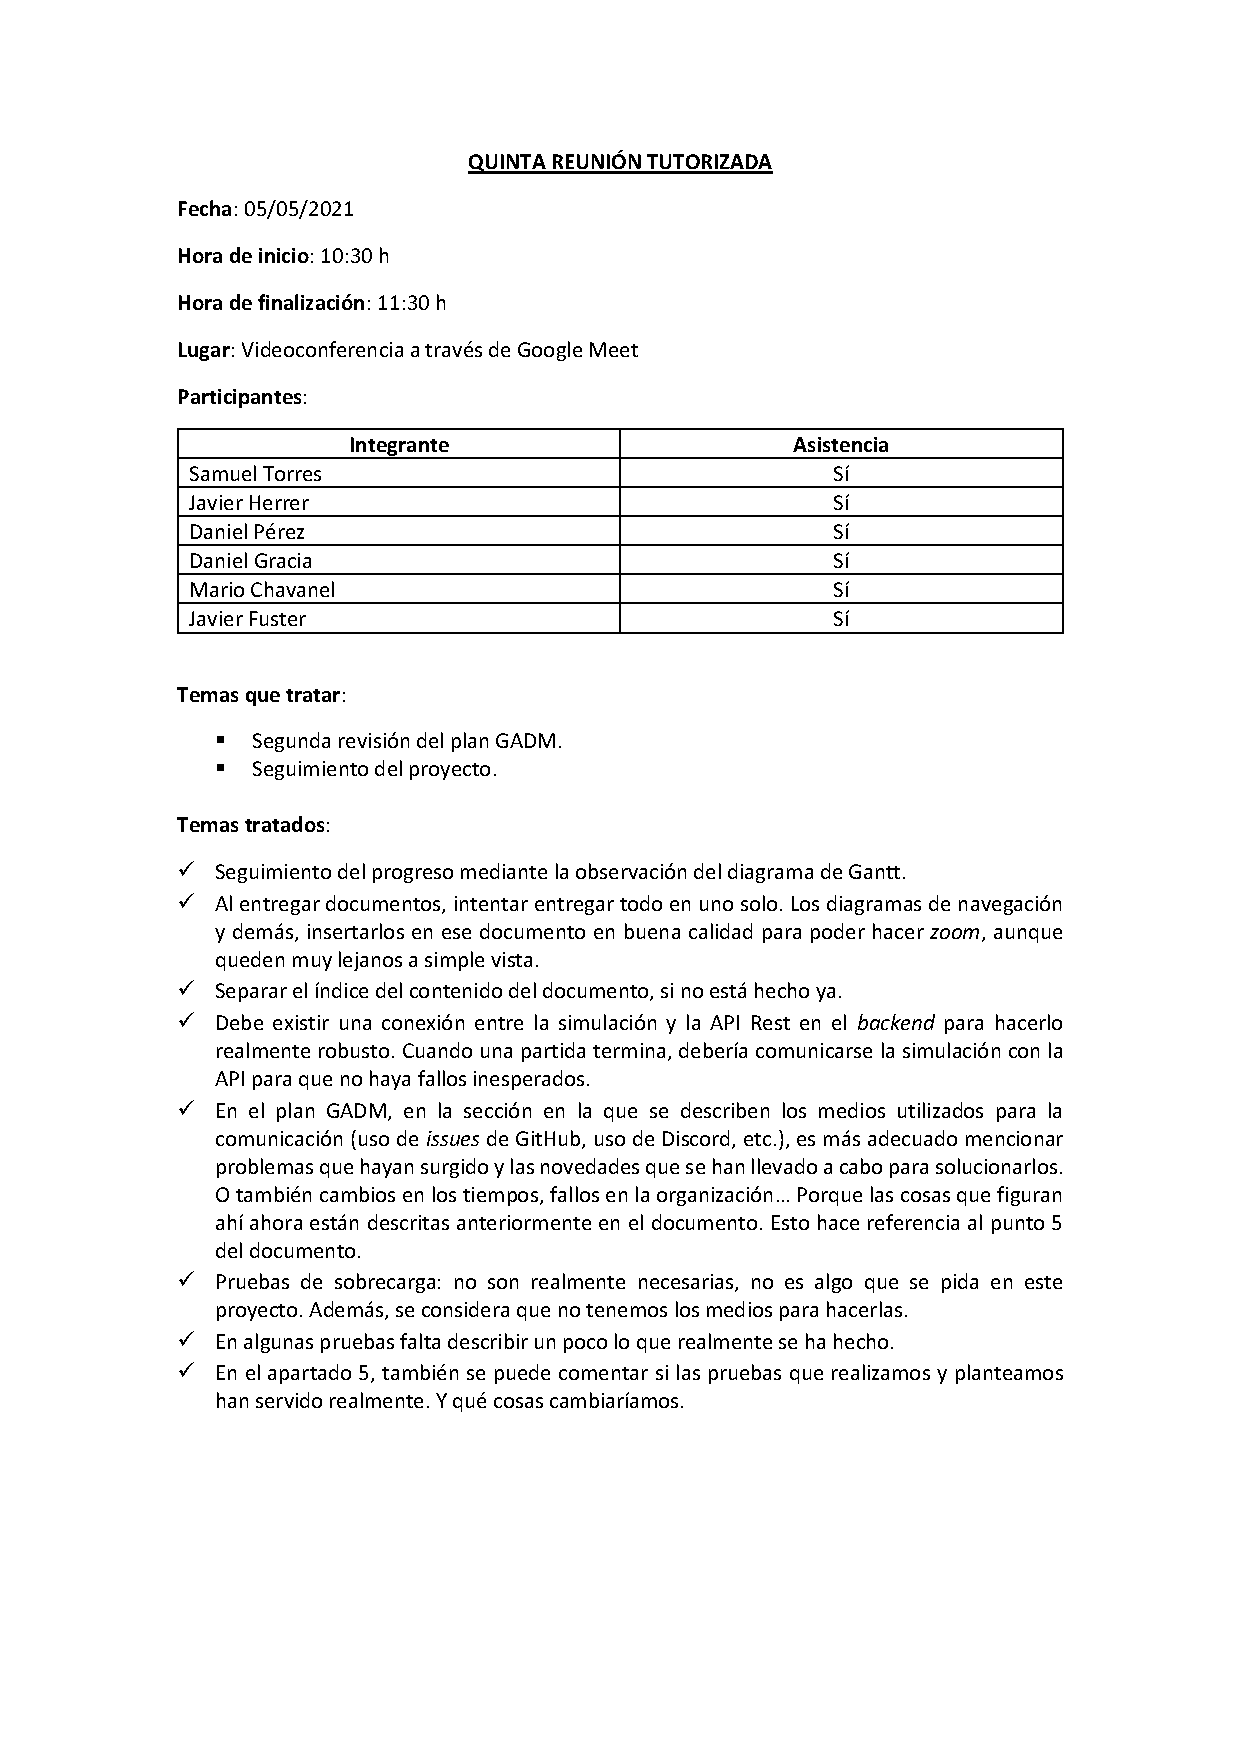
\includegraphics[width=\textwidth]{../images/actas/Acta_reunion_tutorizada_5.pdf}
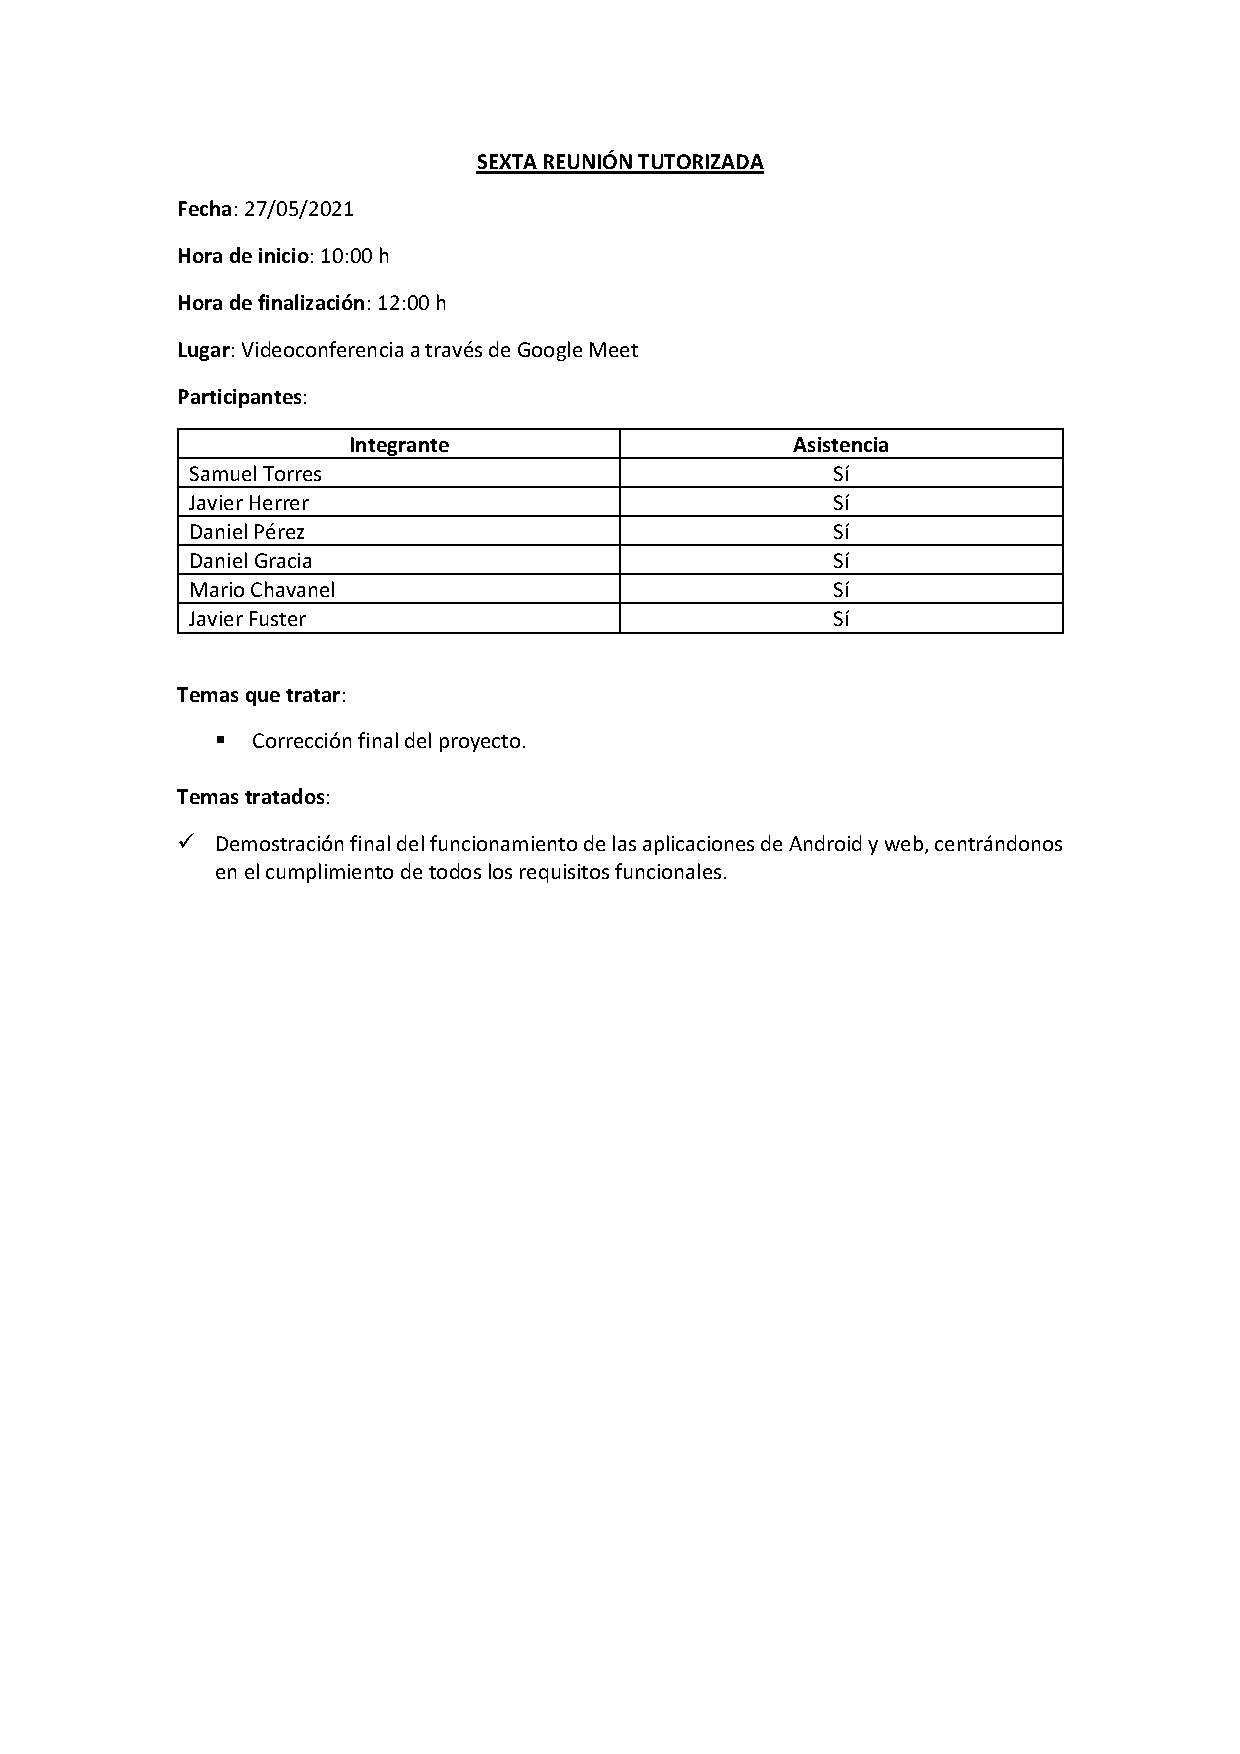
\includegraphics[width=\textwidth]{../images/actas/Acta_reunion_tutorizada_6.pdf}
\break

\FloatBarrier
\section{Anexo: Horas trabajadas} \label{anexo:horas-trabajadas}


\begin{figure}[h]
    \centering
    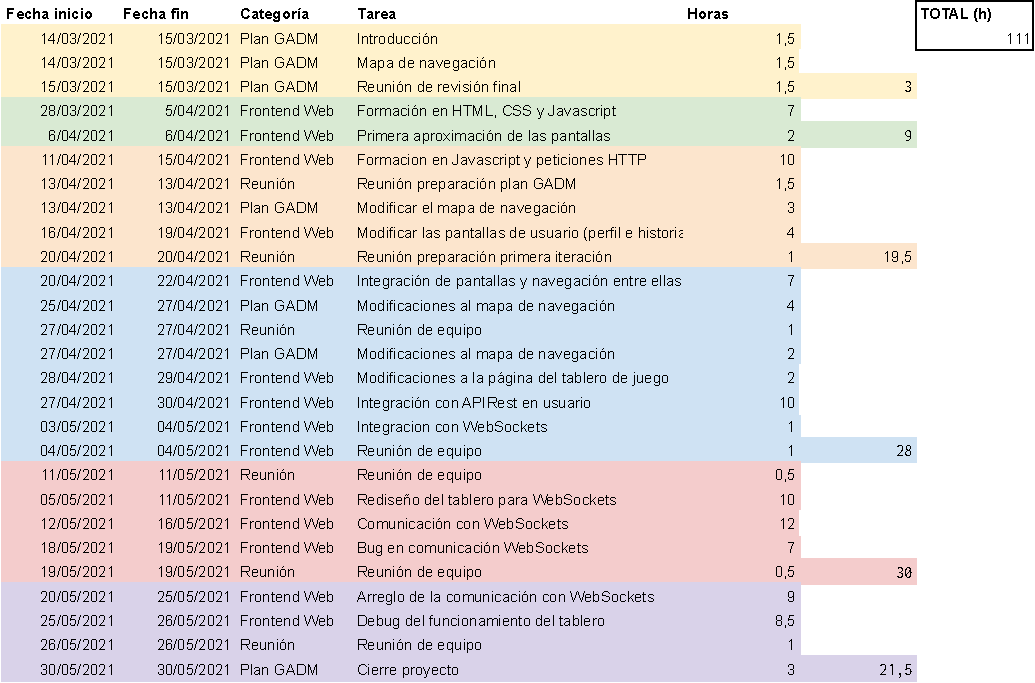
\includegraphics[width=\textwidth]{../images/horasTrabajadas/daniel-gracia.pdf}
    \caption{Daniel Gracia}
\end{figure}

\begin{figure}[h]
    \centering
    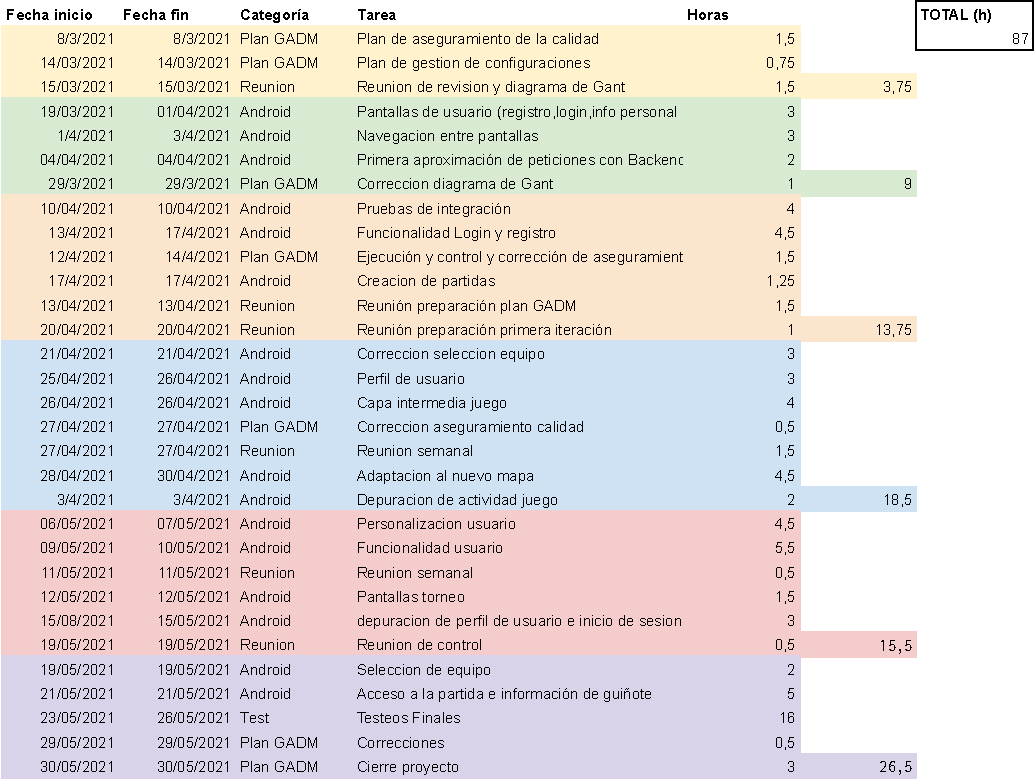
\includegraphics[width=\textwidth]{../images/horasTrabajadas/daniel-perez.pdf}
    \caption{Daniel Pérez}
\end{figure}

\begin{figure}[h]
    \centering
    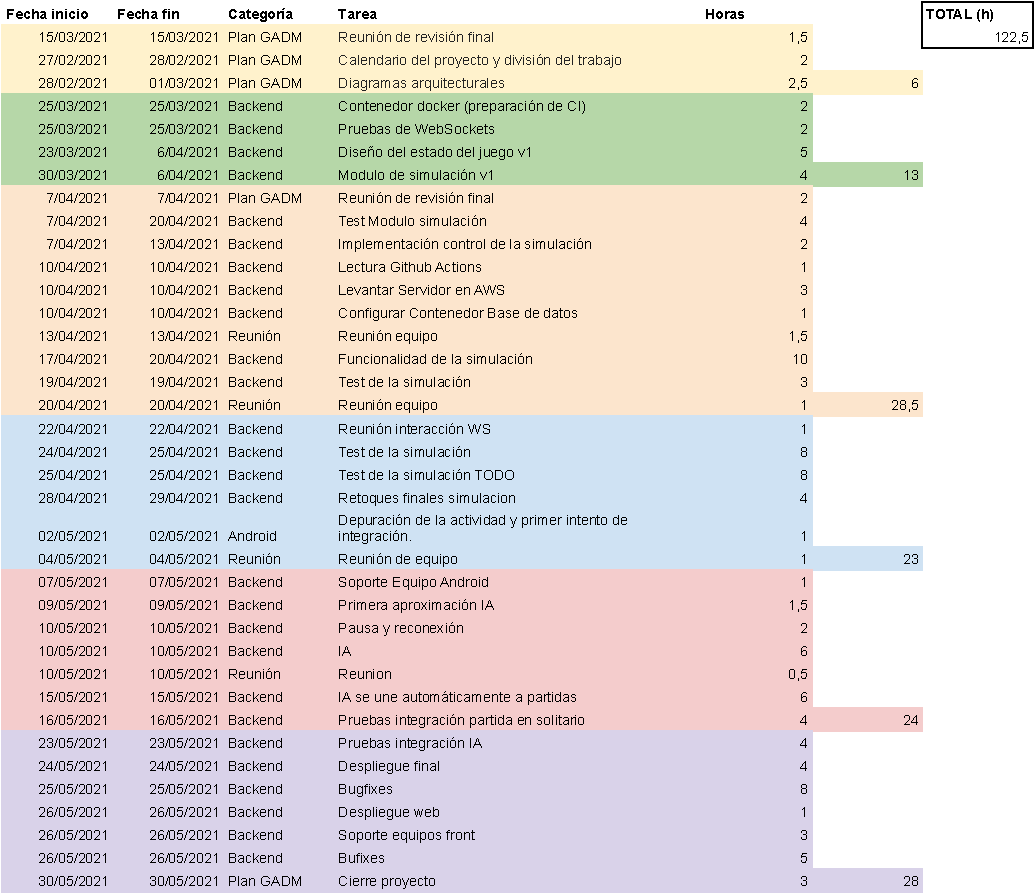
\includegraphics[width=\textwidth]{../images/horasTrabajadas/javier-fuster.pdf}
    \caption{Javier Fuster}
\end{figure}

\begin{figure}[h]
    \centering
    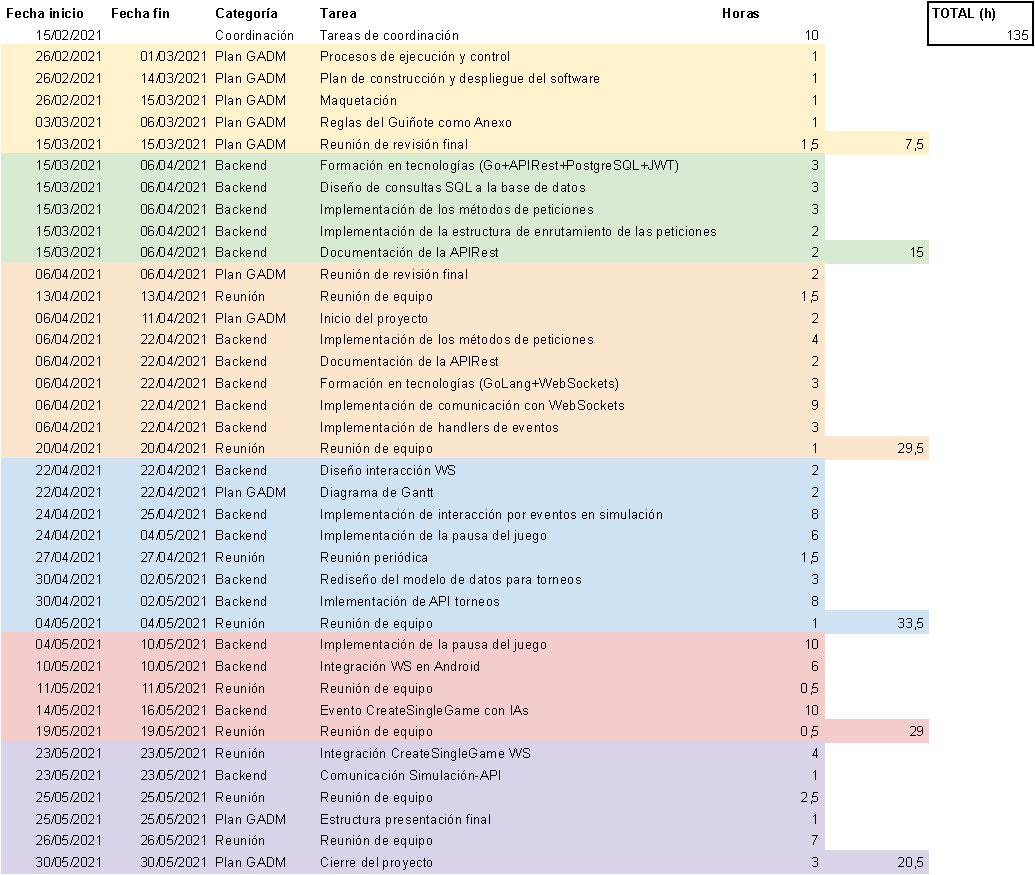
\includegraphics[width=\textwidth]{../images/horasTrabajadas/javier-herrer.pdf}
    \caption{Javier Herrer}
\end{figure}

\begin{figure}[h]
    \centering
    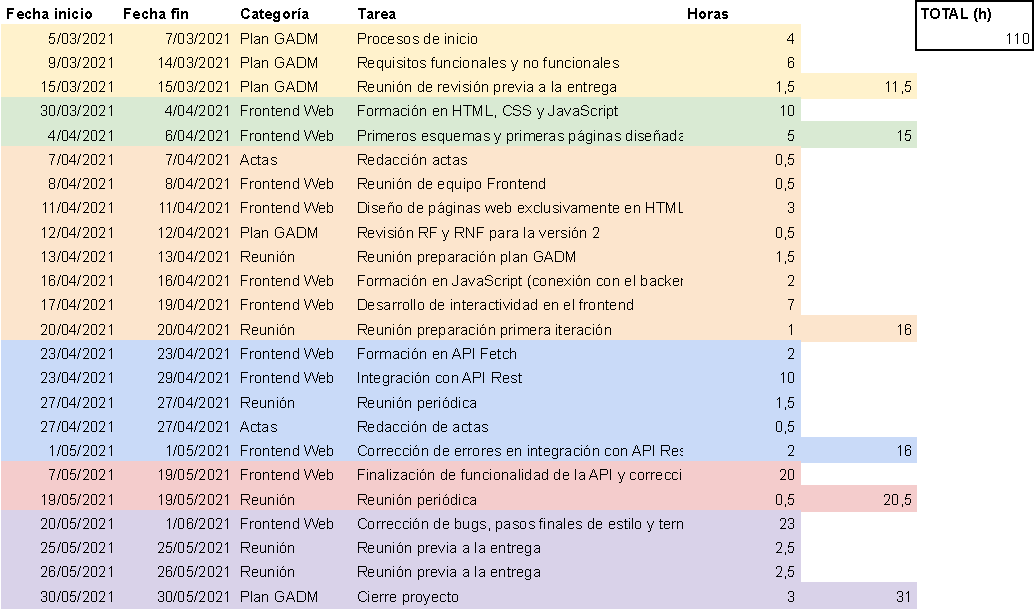
\includegraphics[width=\textwidth]{../images/horasTrabajadas/mario-chavanel.pdf}
    \caption{Mario Chavanel}
\end{figure}

\begin{figure}[h]
    \centering
    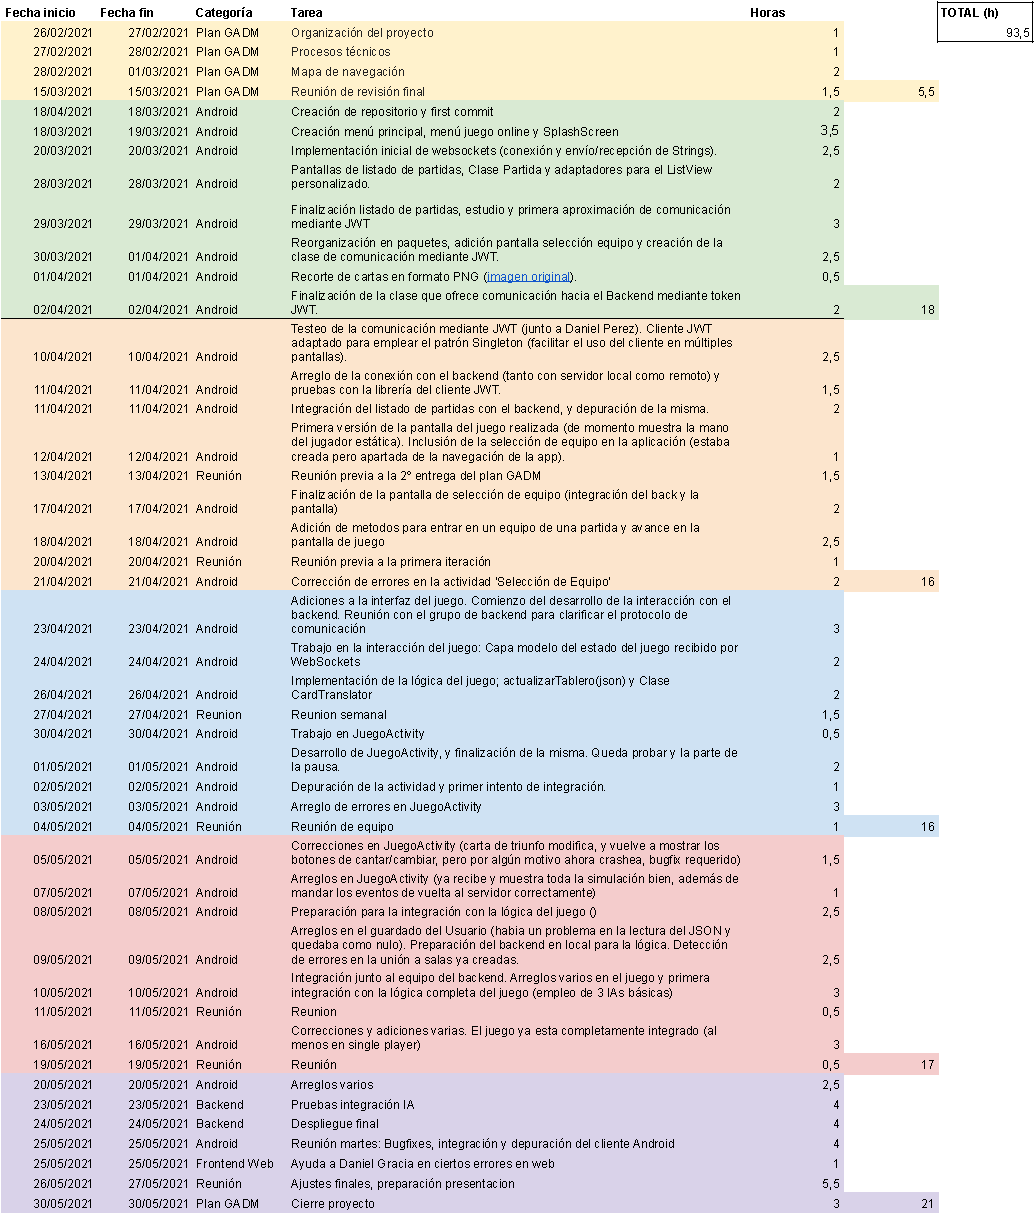
\includegraphics[width=\textwidth]{../images/horasTrabajadas/samuel-torres.pdf}
    \caption{Samuel Torres}
\end{figure}

\FloatBarrier

\section{Anexo: Reglamento del Guiñote}
Fuente: \href{https://www.ludoteka.com/clasika/guinote.html}{Ludoteka.com}

\subsection*{Origen e historia}
El Guiñote es un juego de baraja española perteneciente a la amplia familia del tute, juegos en los que se trata de ir consiguiendo bazas, con un palo dominante o palo de triunfo. El guiñote está especialmente arraigado en Aragón y algunas zonas de Navarra y Castilla.

\subsection*{Descripción}
Se trata de un juego de baraja española de 40 cartas. Se juega entre cuatro personas, formando dos parejas. Dado que las reglas son en muchos aspectos muy similares a las del Tute, en la explicación de las mismas se harán referencias a este último juego.

\subsection*{Objetivo}
El objetivo general del juego es conseguir ganar antes que la pareja rival el número de <<cotos>> pactado inicialmente, cotos constituidos a su vez por el 3 puntos/manos ganadoras. El objetivo concreto para ganar cada una de esas manos es sumar el mayor número de puntos posible con las cartas ganadas en cada baza para superar los 100 tantos necesarios para ganarla. Habrá que intentar llevarse un gran número de bazas que reúnen cartas con la puntuación más alta posible. A estos efectos el valor de cada carta es el que sigue: As (11 puntos), Tres (10 puntos), Rey (4 puntos), Sota (3 puntos) y Caballo (2 puntos). El resto de cartas no tienen valor puntuable.

Existe una jerarquía entre las cartas de un mismo palo de cara a saber cuál es la carta que vence en cada una de las bazas. Es la siguiente, de mayor a menor: As, Tres, Rey, Sota, Caballo, Siete, Seis, Cinco, Cuatro y Dos. A su vez existe una jerarquía entre palos: el palo de mayor rango es el de triunfo (cambia en cada mano), en segundo lugar está el palo de salida (cambia en cada baza), y finalmente están los dos palos restantes.

\subsection*{Desarrollo del juego}
Cada mano tiene dos fases bien diferenciadas. Una primera fase en la que las reglas son muy similares a las del juego de la Brisca y una segunda en la que las reglas son muy similares al propio juego del Tute.
\subsubsection*{Comienzo de la partida y de cada una de las manos}
Se echa a suertes para saber quién es el que reparte por primera vez y quién es mano (el que se sitúe a la derecha del que reparte).

En las siguientes manos será mano el jugador situado a la derecha de quien se llevó las diez de últimas en la mano anterior.

En cada mano el que reparte dará a cortar la baraja al jugador situado a su izquierda, y seguidamente repartirá 6 cartas a cada jugador una a una y de izquierda a derecha. Cuando haya terminado de repartir las cartas, levantará la siguiente dejándola visible junto al mazo durante toda la mano: esa carta será la que pinte, la que marque el triunfo en esa mano.

Cada una de las manos consta de 10 bazas. Una baza es el conjunto de cartas (una por cada jugador) que lanzan sobre el tapete los jugadores en su turno respectivo. Cada vez que se completa una baza habrá un jugador que la gana, que se la lleva.
\subsubsection*{Primera fase de la mano}
Mientras queden cartas en el mazo (durante las cuatro primeras manos), el que va de mano echará al centro del tapete una de sus cartas (la que él quiera), y los demás, de izquierda a derecha, deberán echar una más cada uno, la que ellos quieran, sin limitaciones u obligaciones de ningún tipo respecto a cuál echar.

\subsubsection*{Recoger las bazas}

La baza se la llevará el jugador que hubiera echado la carta más alta del palo de triunfo, y si no hay triunfos sobre el tapete, la carta más alta del palo de salida.

En las bazas sucesivas, dentro de una misma mano, el jugador que se ha llevado la última baza es el que empezará lanzando la 1ª carta de la baza siguiente.

Antes de lanzar nuevamente las cartas para jugar una nueva baza, todos los jugadores tomarán una carta de encima del mazo, empezando por el que ganó la baza anterior, de forma que siempre tengan seis cartas en la mano.

\subsubsection*{Cambio de cartas}

Cuando un jugador tuviera en su mano durante el juego el siete del palo de triunfo, podrá cambiarlo por la carta que pinte si ésta fuera una carta de valor (As, Tres, Rey, Sota o Caballo). Este cambio podrá hacerse justo tras haber ganado una baza y antes de proceder a robar la carta correspondiente del mazo.

Para obtener el cambio de carta debe pulsarse en cualquier momento la carta que marca el triunfo, de modo que el programa realiza el cambio en cuanto éste es posible.

\subsubsection*{Segunda fase de la mano o fase de Arrastre}

Lógicamente, conforme avance el juego en una mano, las cartas del mazo se acabarán y llegará un momento en que no habrá cartas para robar: en las seis últimas bazas se jugará sólo con las cartas que tuvieran en la mano. Cuando las cartas del mazo se acaban, el último jugador toma la carta que señala el palo de triunfo.

En esta fase cambian las normas en cuanto a obligatoriedad al echar cartas, pasando a utilizar las normas del tute (con alguna pequeña diferencia). El jugador que hubiera ganado la última baza de la fase anterior echa al centro del tapete una de sus cartas (la que él quiera), que será la que indique el palo de salida de esa baza, y los demás, de izquierda a derecha, deberán echar una más cada uno, siguiendo las reglas siguientes:

\begin{itemize}
	\item Obligación de \textbf{montar} y de \textbf{asistir}: si un jugador, en su turno, tuviera cartas del palo de salida estará obligado a ASISTIR (echar carta de ese palo), y además, si pudiera, a MONTAR (echar una carta del palo de salida que supere a las cartas que están sobre el tapete).
	\item Obligación de \textbf{fallar}: si un jugador, en su turno, no pudiera asistir (no tuviera carta del palo de salida) deberá FALLAR (echar una carta del palo de triunfo) siempre que superase a las que hubiera sobre el tapete.
	\item Si la baza la va ganando la pareja no hay obligación de montar ni fallar, sino tan sólo la obligación de asistir al palo de salida. Ésta es una particularidad que distingue al Guiñote del Tute en esta fase del juego.
	\item Si un jugador no tuviera cartas para asistir ni para fallar superando las cartas del tapete, podrá entonces echar la carta que quiera.
	\item La baza se la llevará el jugador que hubiera echado la carta más alta en la jerarquía arriba indicada.
	\item En las bazas sucesivas, dentro de una misma mano, el jugador que se ha llevado la última baza es el que empezará lanzando la 1ª carta de la baza siguiente.
\end{itemize}

\subsubsection*{Cánticos}

Durante el desarrollo de la mano, si un jugador tuviera el rey y la sota de un mismo palo, podrá realizar un cántico, es lo que se denomina cantar las 40 (si se trata de la sota y el rey del palo de triunfo) o cantar las 20 (si se trata de rey y sota de cualquier otro palo). Deberá indicar tal circunstancia precisando el palo en el que canta las 20 (20 en oros, copas, espadas o bastos) o si canta las 40 bastará que lo indique sin necesidad de indicar el palo, ya que en cada mano sólo existe un palo de triunfo. Si el cántico se hace durante la fase de arrastre, no es necesario indicar el palo del que se trata, salvo que así lo solicite el propio compañero, en cuyo caso sí deberá indicarse el palo concreto.

Los cánticos asignan los tantos que indican sus nombres (20 ó 40) a efectos del recuento final de la mano.

Los cánticos pueden realizarse cuando la propia pareja ha realizado la última baza.

\subsubsection*{Puntuación por las bazas}

Una vez que se han completado todas las bazas de una mano, se procederá al recuento de los puntos obtenidos por cada jugador en esa mano por las bazas ganadas, que se sumarán a los ya obtenidos por razón de los cánticos.

Los tantos serán sumados a todos los efectos por parejas.

La pareja que hubiera llevado la última baza de una mano sumará 10 tantos más (10 de últimas)

El número total de puntos que suman las cartas de la baraja es 120. Lógicamente, además, en todas las manos habrá 10 puntos de últimas. Por otro lado, el máximo de puntos posible por razón de los cánticos es 100.

La pareja que supere los 100 tantos ganará la mano.

Si ambas parejas superan dicha cantidad no gana necesariamente la qué más tantos haya obtenido:

\begin{itemize}
	\item Si una pareja no alcanza 30 puntos sin contar los cantes, pierde
	\item Si ambas parejas además de superar los 100 tantos, superan los 30 tantos sin contar los cantes, gana quien se lleva las 10 últimas.
\end{itemize}

Si ninguna de las parejas supera los 100 tantos en una mano se jugará una mano más llamada "de vueltas". No es preciso que en la mano de vuelta sean jugadas todas las cartas, sino que el ganador de cada baza tiene la opción de anunciar que ha superado los 100 puntos, dándola así por finalizada. Si efectivamente, sumando los puntos de la mano anterior, supera los 100 puntos, la mano es suya; en caso contrario, será para la pareja oponente.

\subsection*{Final de la partida}

Gana la partida aquella pareja que antes consiga alcanzar el número de cotos pactado inicialmente, formado a su vez por tres manos/puntos.

\section{Anexo: Diagrama de Gantt} \label{anexo:Gantt}

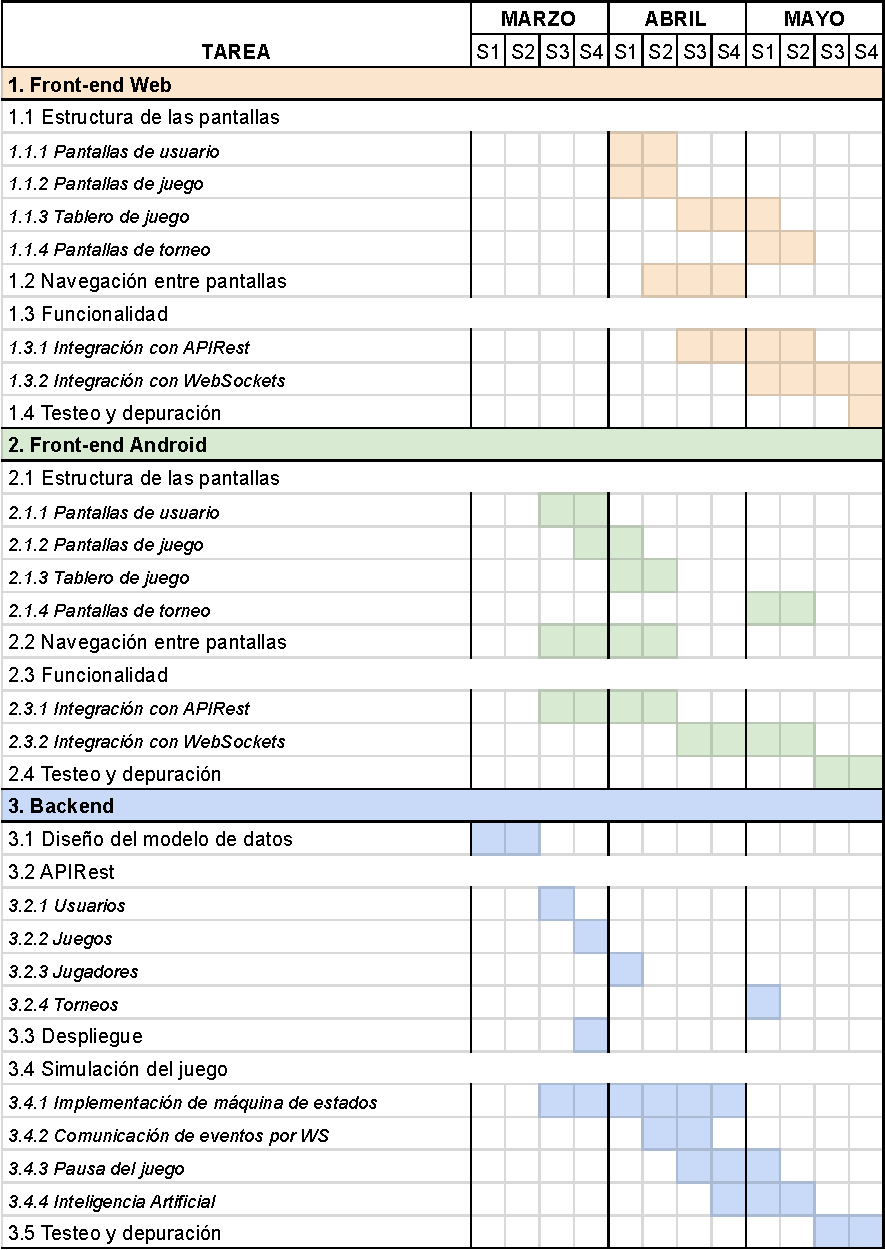
\includegraphics[width=\textwidth]{../images/diagramaGantt}
\begin{landscape}
    \section{Anexo: Mapa de navegación} \label{anexo:navegacion}

    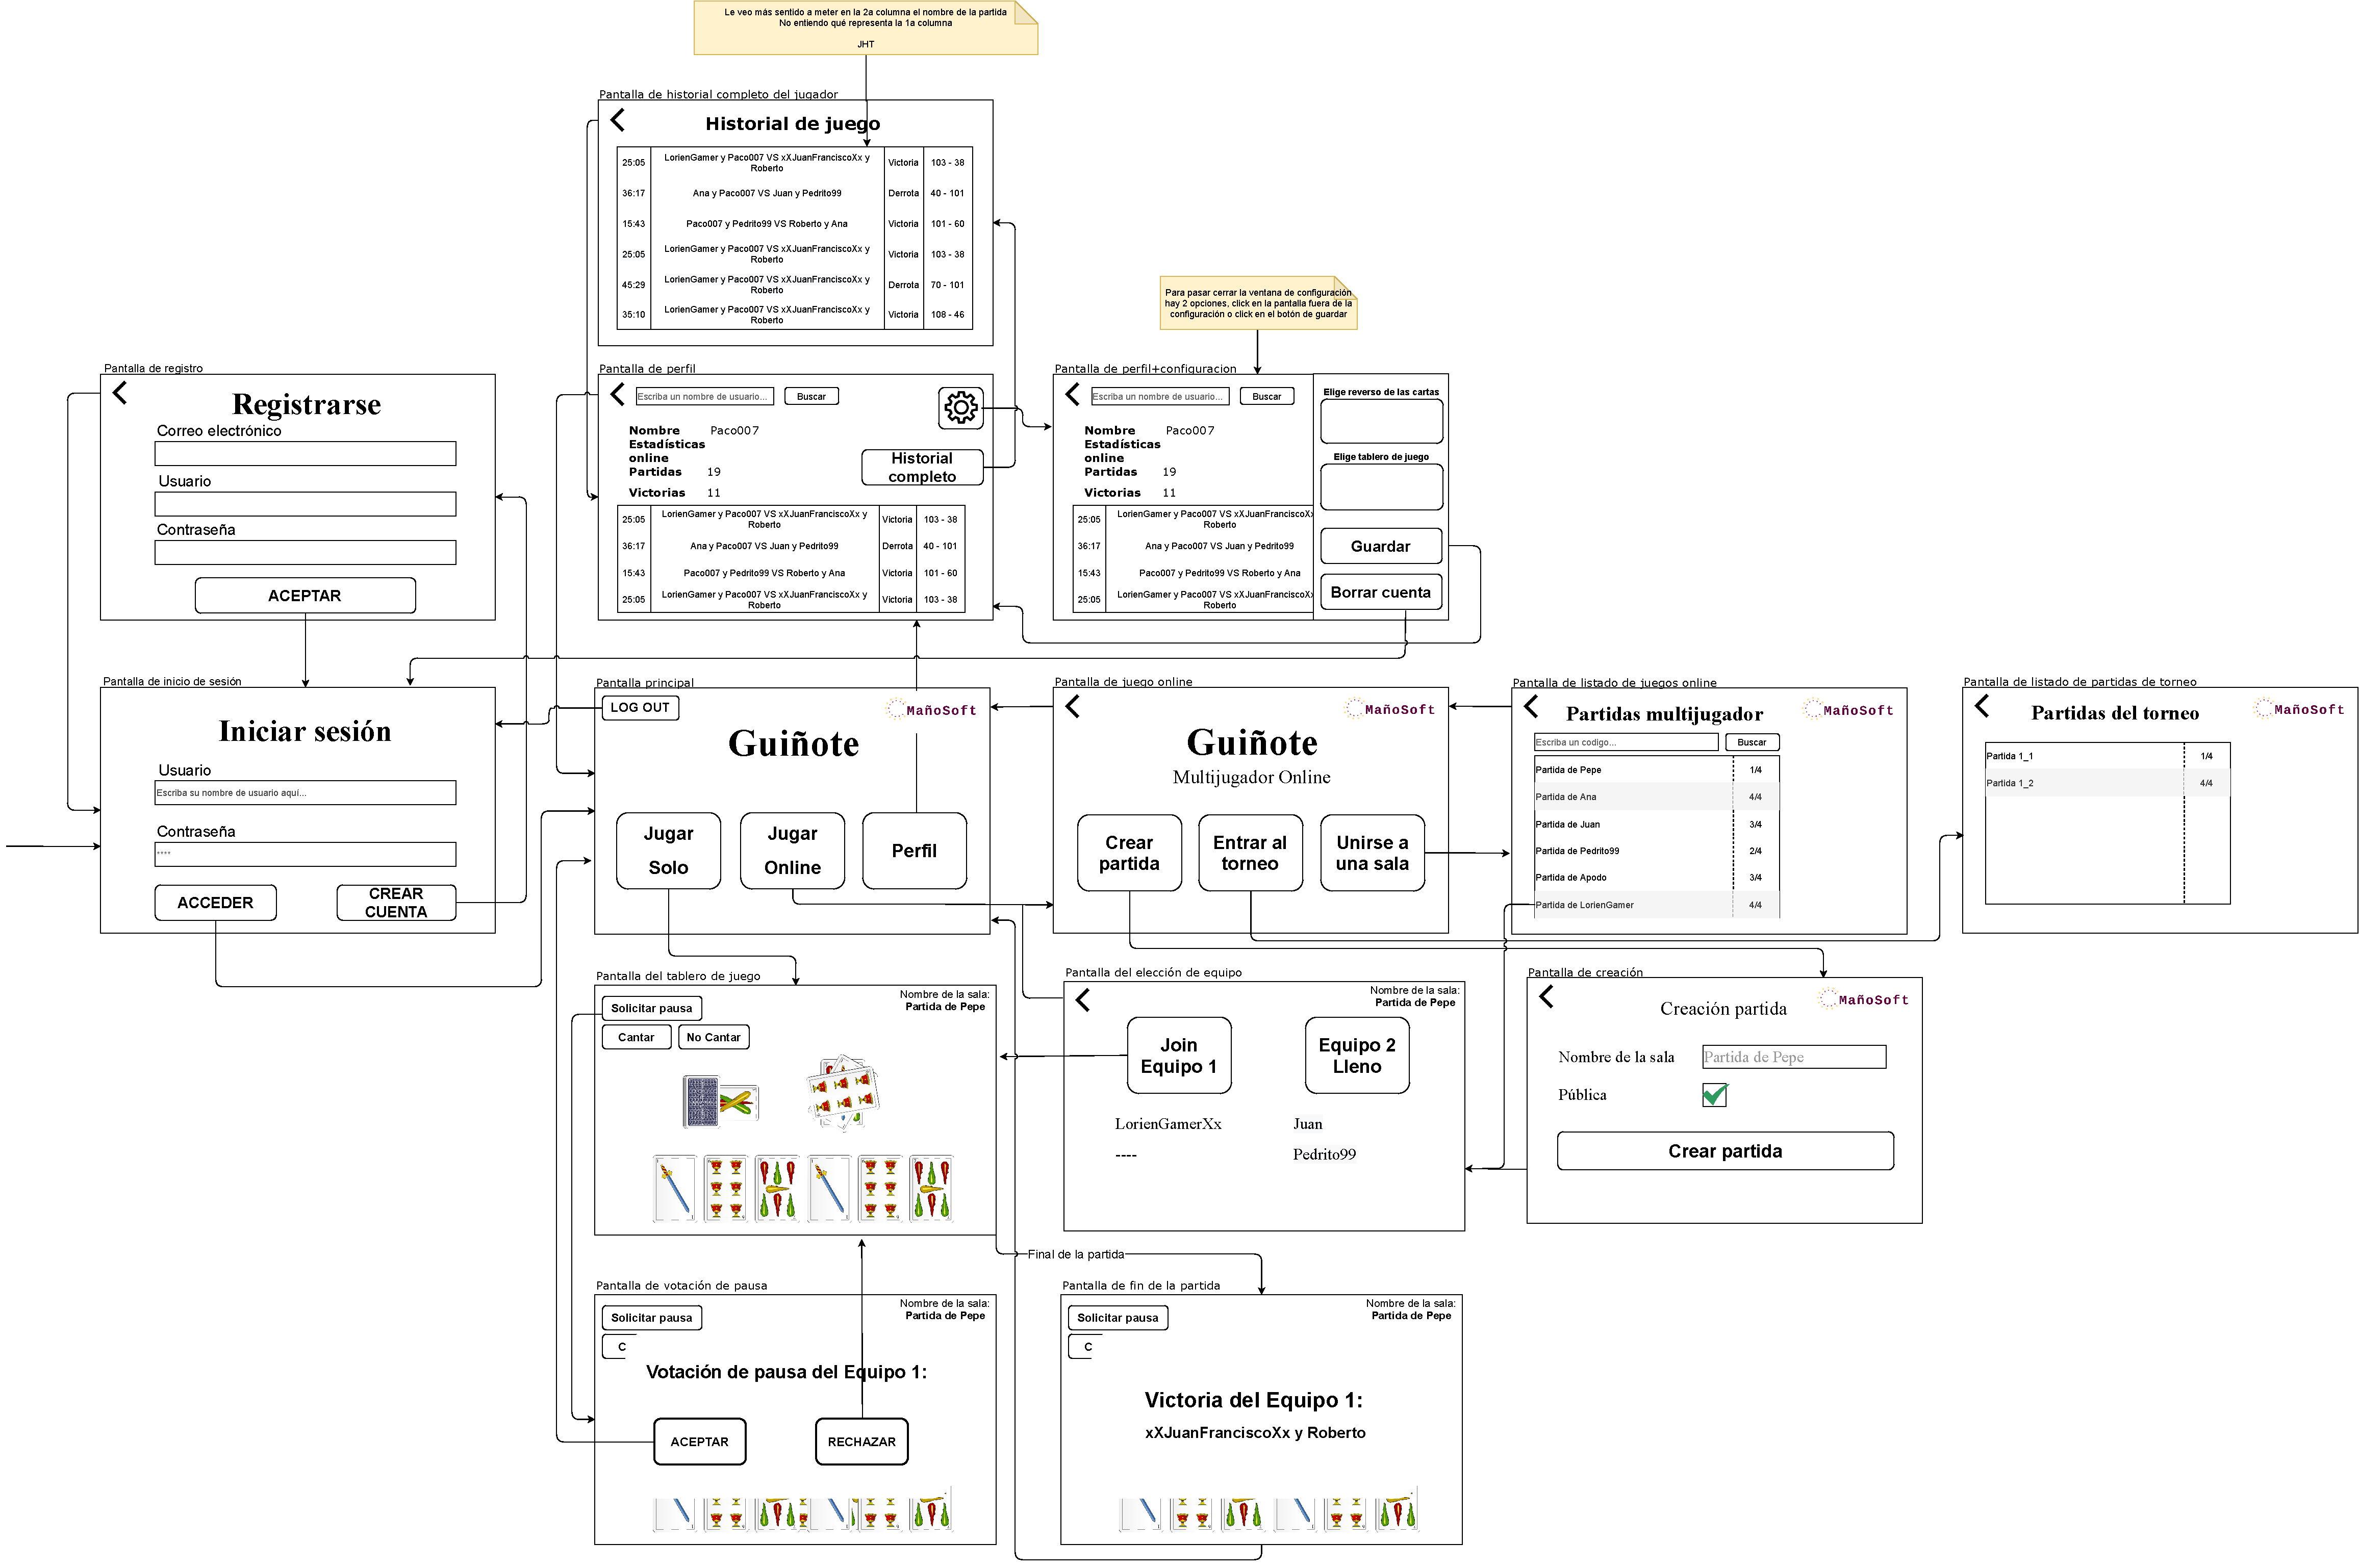
\includegraphics[width=1.5\textwidth]{../images/mapaNavegacion}

    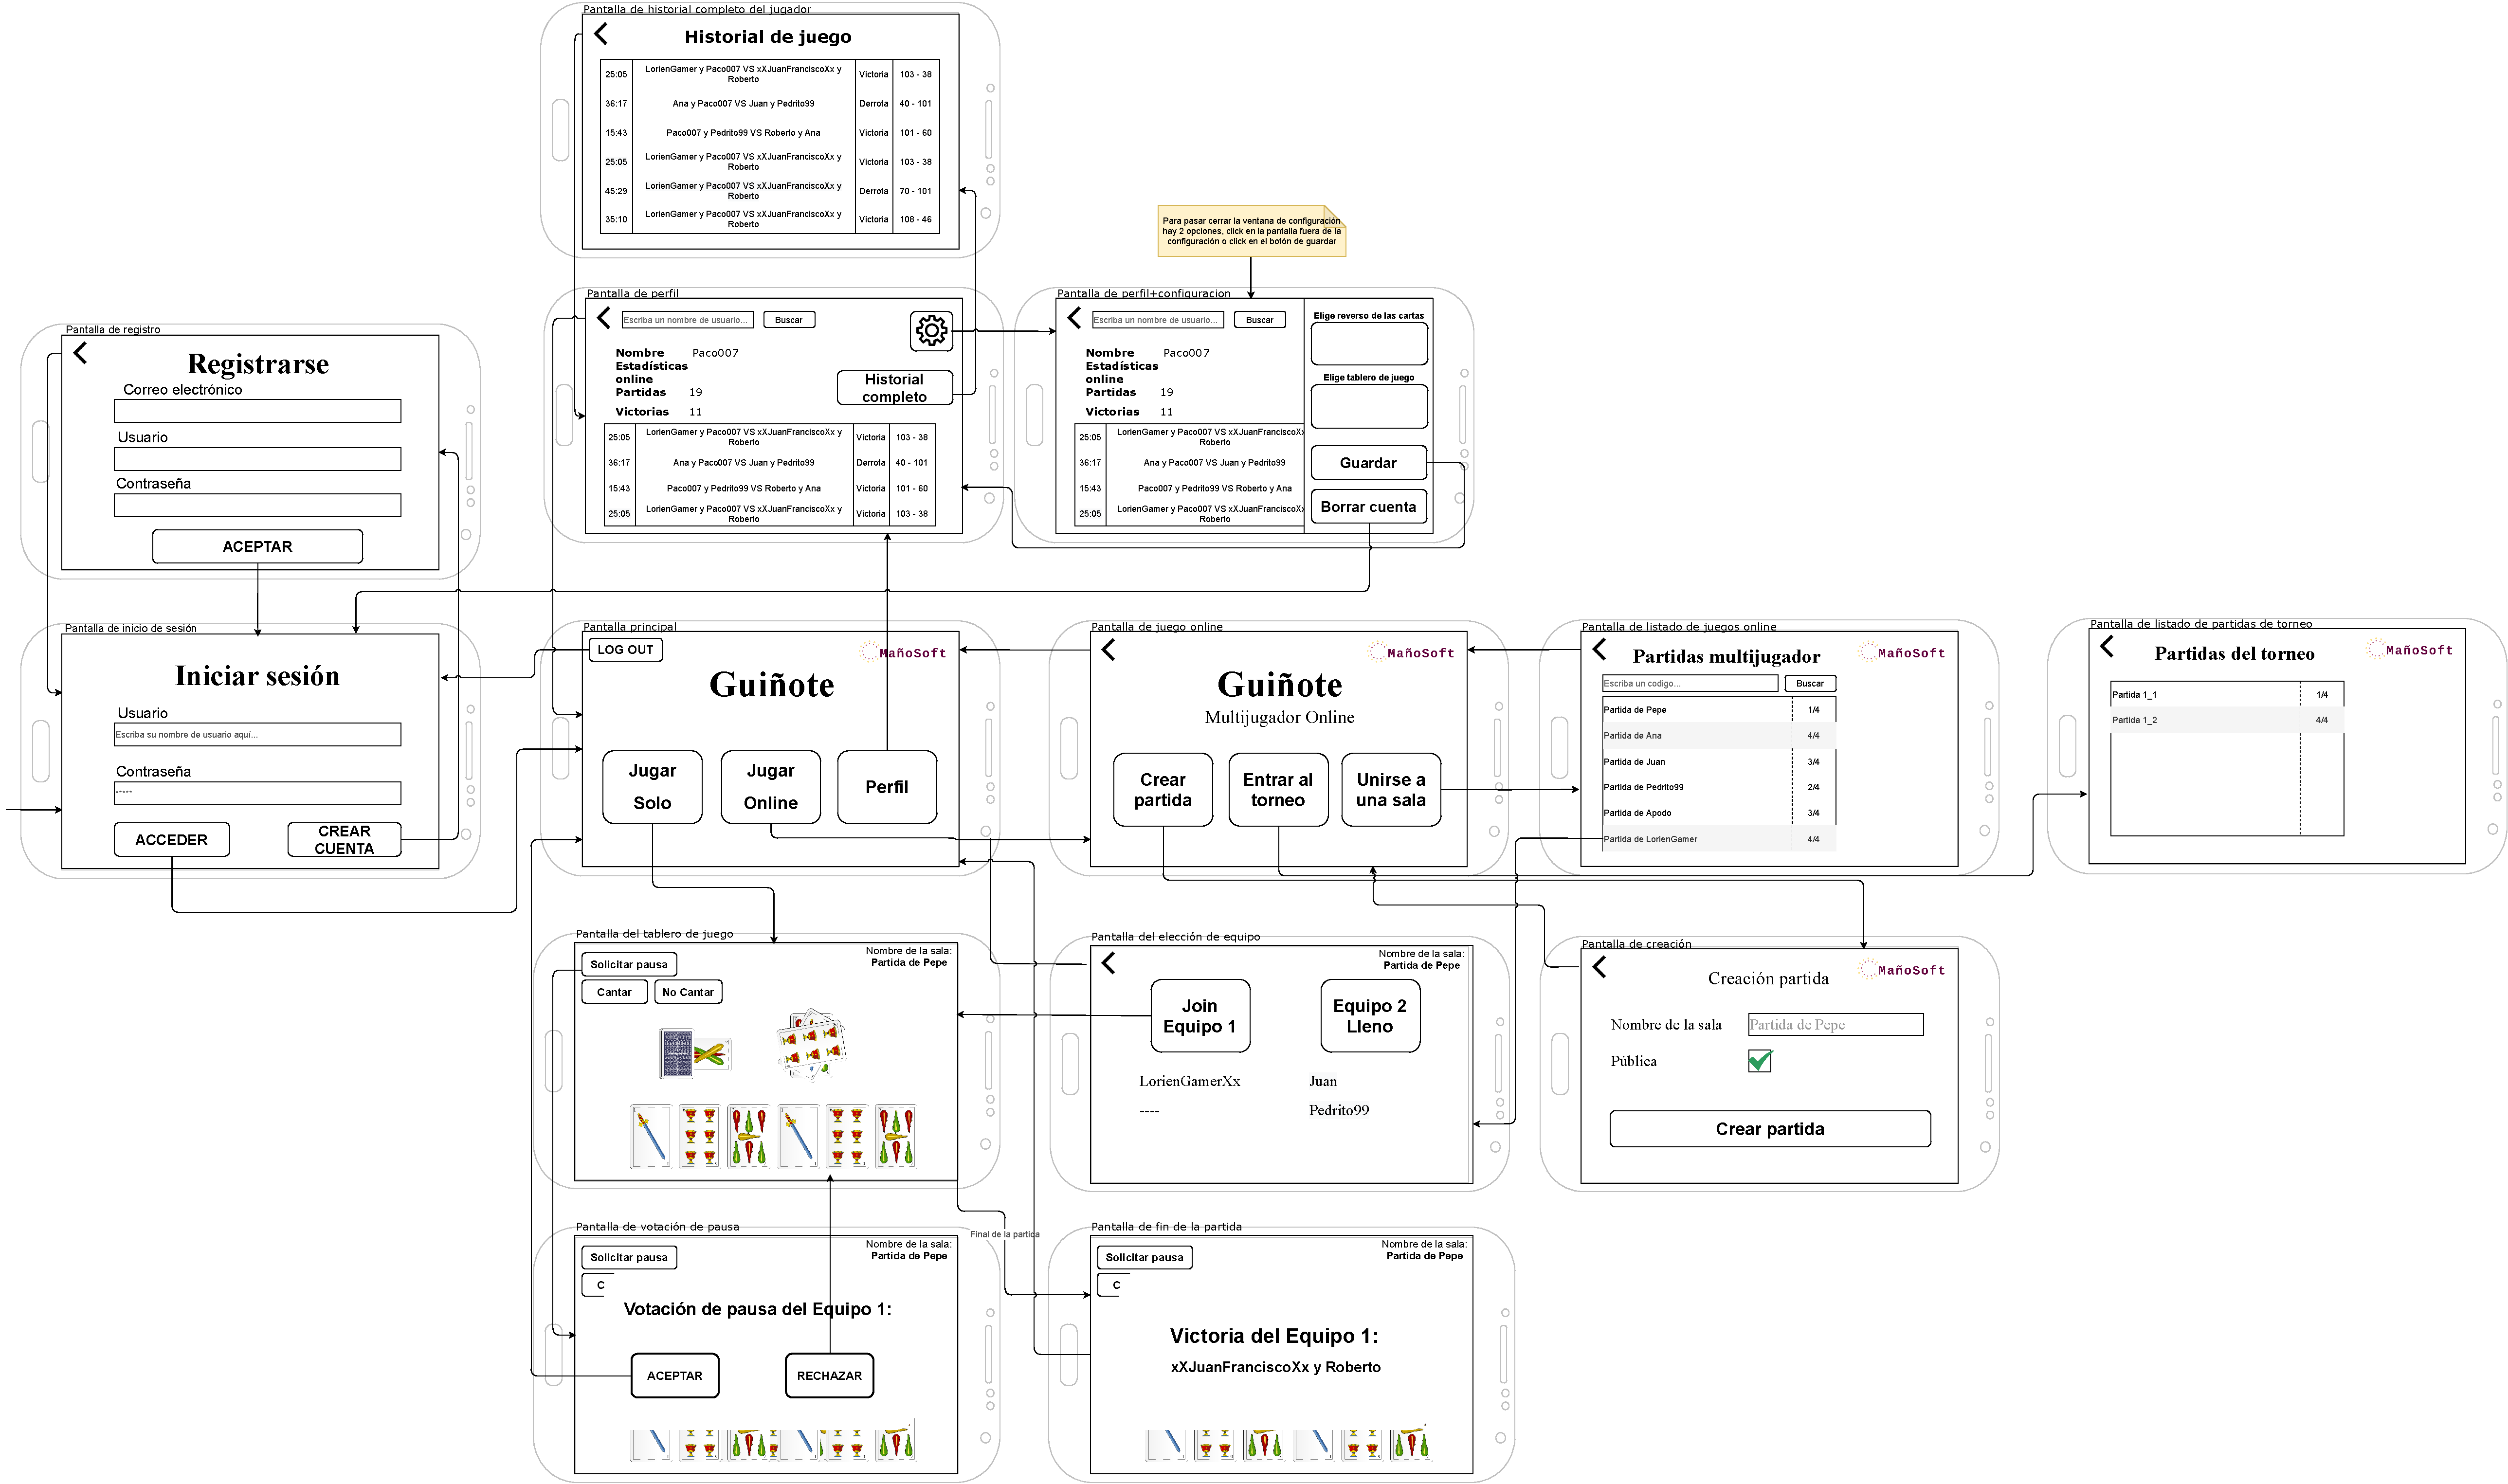
\includegraphics[width=1.5\textwidth]{../images/mapaNavegacionAndroid}

\end{landscape}

\section{Anexo: Diagramas de secuencia}

\begin{figure}[h]
    \centering
    \includegraphics[width=0.9\textwidth]{../images/diagramasSecuencia/Interacción-Create&Join}
    \caption{Crear y unirse a una partida}
\end{figure}

\begin{figure}[h]
    \centering
    \includegraphics[width=0.9\textwidth]{../images/diagramasSecuencia/Interacción-SingleGameCreate}
    \caption{Jugar una partida en solitario}
\end{figure}

\begin{figure}[h]
    \centering
    \includegraphics[width=\textwidth]{../images/diagramasSecuencia/Interacción-Join}
    \caption{Unirse a una partida}
\end{figure}

\begin{figure}[h]
    \centering
    \includegraphics[width=\textwidth]{../images/diagramasSecuencia/Interacción-Pause}
    \caption{Pausa de un juego}
\end{figure}

\begin{figure}[h]
    \centering
    \includegraphics[width=\textwidth]{../images/diagramasSecuencia/Interacción-Rejoin}
    \caption{Retormar una partida pausada}
\end{figure}

\FloatBarrier

\section{Anexo: Diagrama de estados simulación}

\begin{figure}[h]
    \centering
    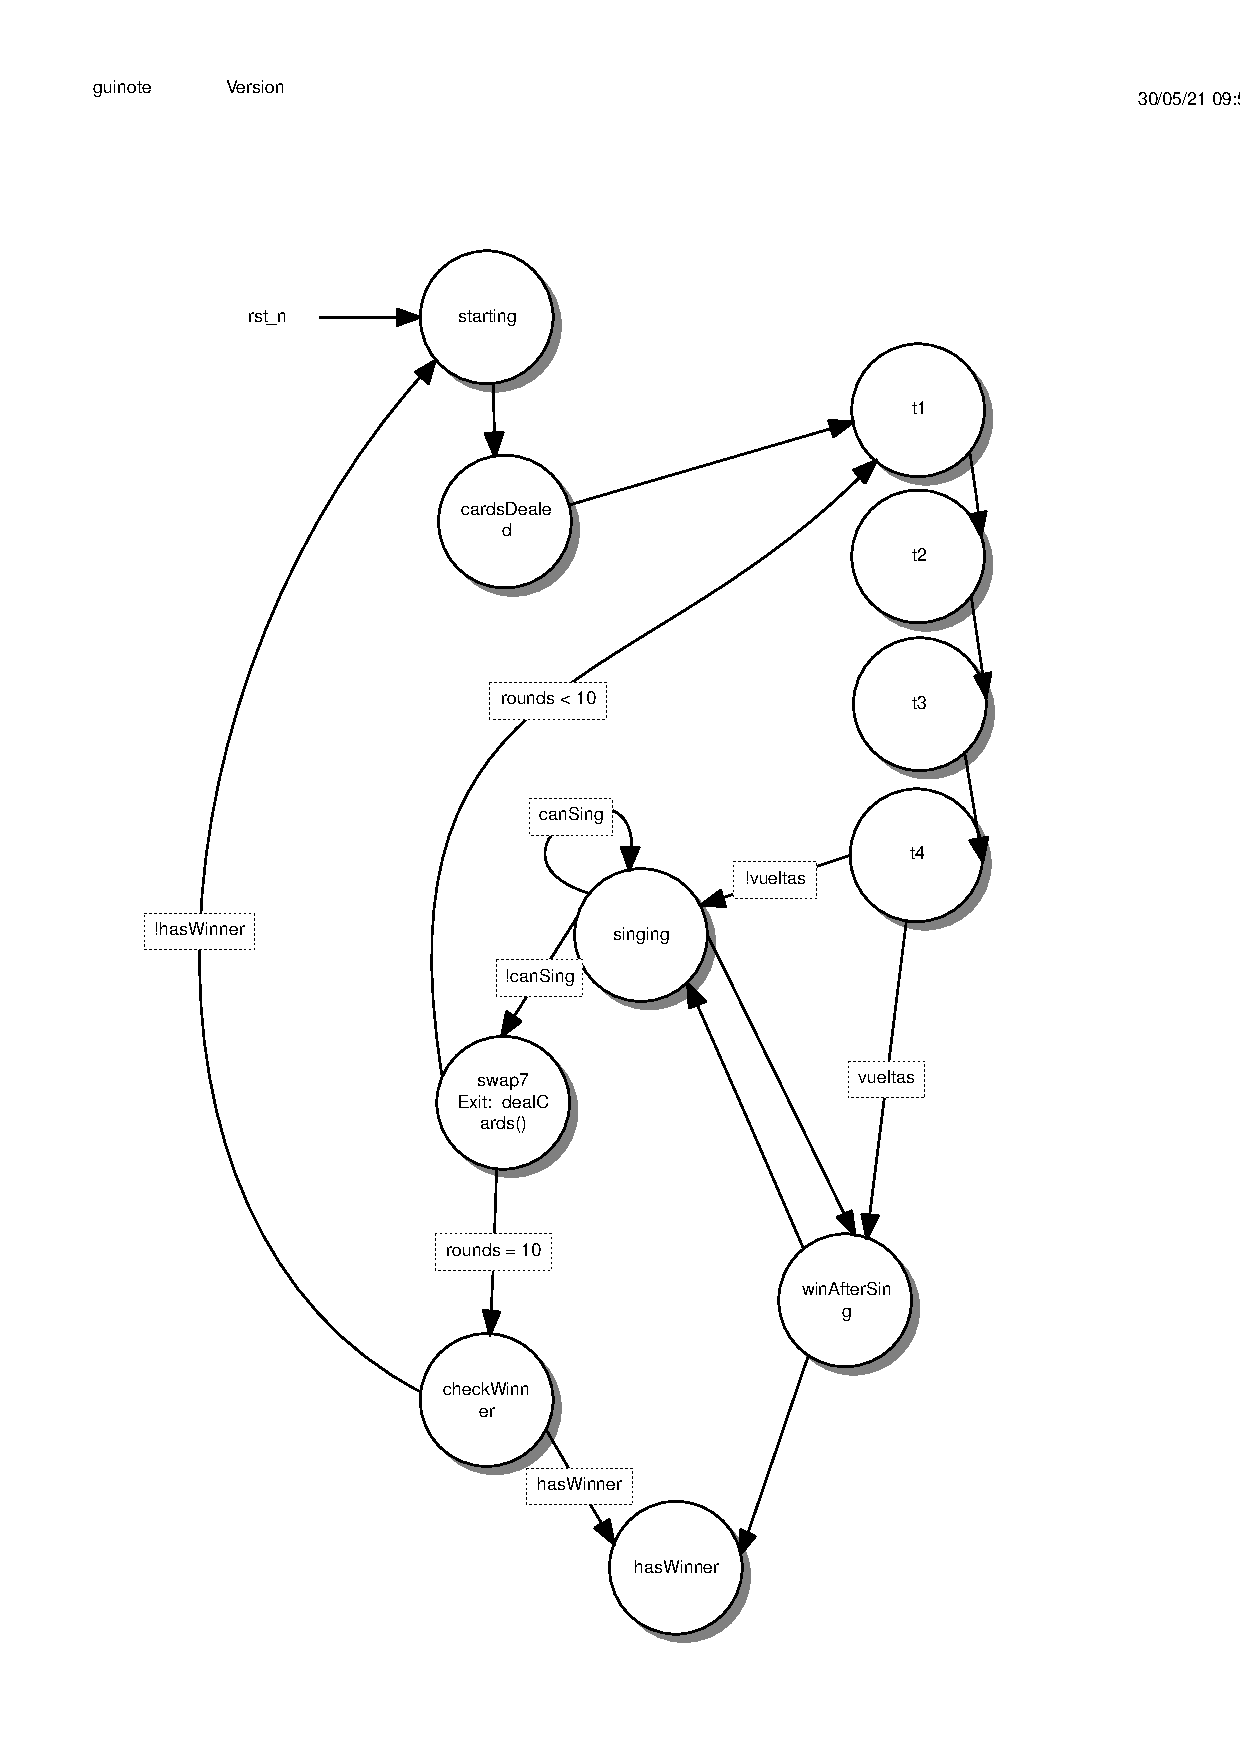
\includegraphics[width=0.75\textwidth]{../images/diagrama_estados.pdf}
    \caption{Retormar una partida pausada}
\end{figure}

\end{document}
